\documentclass[10pt]{beamer}
\usetheme{Boadilla}% theme général du diaporam
% paquets pour le français
\usepackage[T1]{fontenc}
\usepackage[utf8]{inputenc}
\usepackage{pgf}
\usepackage{color}
\usepackage{lmodern}
\usepackage{tikz}
\usepackage{eurosym}
\usepackage{verbatim}
\usepackage{multicol}
\usepackage[eulergreek,EULERGREEK]{sansmath}
\definecolor{nemo}{rgb}{1.,0.27,0.} 
\setbeamercolor{structure}{fg=nemo}
\setbeamercolor{alerted text}{fg=blue}
\usepackage{array}

\setbeamertemplate{footline}[text line]
{
  \insertshortauthor\\ \insertshortdate \hfill  \small{\insertpagenumber}
}

\makeatletter
\newcommand{\boldarrayrulewidth}{1\p@} 
\def\bhline{\noalign{\ifnum0=`}\fi\hrule \@height  
 \boldarrayrulewidth \futurelet \@tempa\@xhline}

\def\@xhline{\ifx\@tempa\hline\vskip \doublerulesep\fi
 \ifnum0=`{\fi}}
\newcommand{\ms}{\noalign{\vspace{3\p@ plus2\p@ minus1\p@}}}

\makeatother
\newcommand{\br}{\ms\bhline\ms}
\newcommand{\mr}{\ms\hline\ms}

\begin{document}

\title{\textbf{Bayesian Inference of Formation Energies}} 
\author{Sophie Blondel \& Crystal Jernigan}  
\date{\today}

\frame{\titlepage}

% \begin{frame}{Formation Energy Data}
% 	Formation energy files only for V~$= 1, 2, 6, 14, 18, 19, 27, 32, 44$. \newline
% 	
% 	Example:
% 	
% 	\texttt{\#V \#He Ef \\
% 	1 ~0  ~~3.82644  \\                                                                                           
% 	1 ~1  ~~5.14166  \\                                                                                        
% 	1 ~2  ~~8.20919  \\                                                                                         
% 	1 ~3  ~~11.5304} \newline
% 	
% 	Binding energy formula:
% 	$$\text{E}_{\text{b}}(\text{He}_{\text{X}}, \text{V}_{\text{Y}}) =
% 	\text{E}_{\text{f}}(\text{He}_{\text{X}-1}, \text{V}_{\text{Y}}) +
% 	\text{E}_{\text{f}}(\text{He}_1, 0) -
% 	\text{E}_{\text{f}}(\text{He}_{\text{X}}, \text{V}_{\text{Y}})$$
% \end{frame}
% 
% \begin{frame}{Binding Energy Data}
% 	Binding energy file for V up to $50$. \newline
% 	
% 	Example:
% 	
% 	\texttt{\#He \#V \#I E\_He ~~~~E\_V ~~~~~E\_I ~~~~~E\_t ~~~~~E\_mig
% 	~~~D\_0
% 	\\
% 	1 ~~0 ~0 ~Infinity Infinity Infinity 8.270E+0 1.300E-1 2.950E+10 \\
% 	2 ~~0 ~0 ~8.640E-1 Infinity Infinity 6.120E+0 2.000E-1 3.240E+10 \\
% 	3 ~~0 ~0 ~1.210E+0 Infinity Infinity 4.440E+0 2.500E-1 2.260E+10 \\
% 	4 ~~0 ~0 ~1.560E+0 Infinity Infinity 3.180E+0 2.000E-1 1.680E+10 } \newline
% 	
% 	Here we are only interested in the helium binding energy.
% \end{frame}
% 
% \begin{frame}{Helium Formation Energy}
% 	$\text{E}_{\text{f}}(\text{He}_1, 0)$ is missing from our data:
%     \begin{itemize}
%       	\item[$\blacktriangleright$] can be computed with the formula and the
%       	data we have.
%     \end{itemize}
% 	$$\text{E}_{\text{b}}(\text{He}_{\text{X}}, \text{V}_{\text{Y}}) =
% 	\text{E}_{\text{f}}(\text{He}_{\text{X}-1}, \text{V}_{\text{Y}}) +
% 	\text{E}_{\text{f}}(\text{He}_1, 0) -
% 	\text{E}_{\text{f}}(\text{He}_{\text{X}}, \text{V}_{\text{Y}})$$
% 	
%     \begin{figure}
%         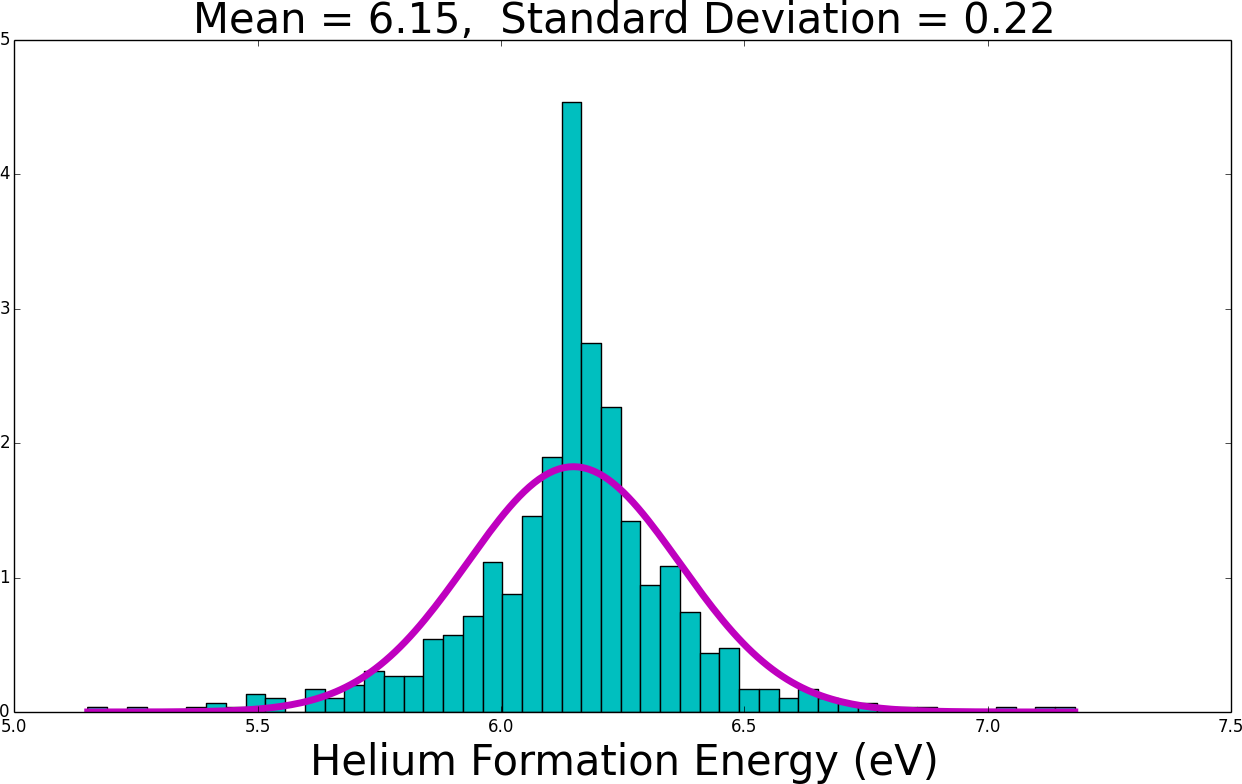
\includegraphics[width=0.7\textwidth]{heliumFormation}
%     \end{figure}
% 	
% 	$\text{E}_{\text{f}}(\text{He}_1, 0) = 6.15$~eV will be used now.
% \end{frame}
% 
% \begin{frame}{Rebuilding Binding Energies}
% 	Using only the given formation energies, one can now compute new binding
% 	energies:
% 	
%     \begin{figure}
%         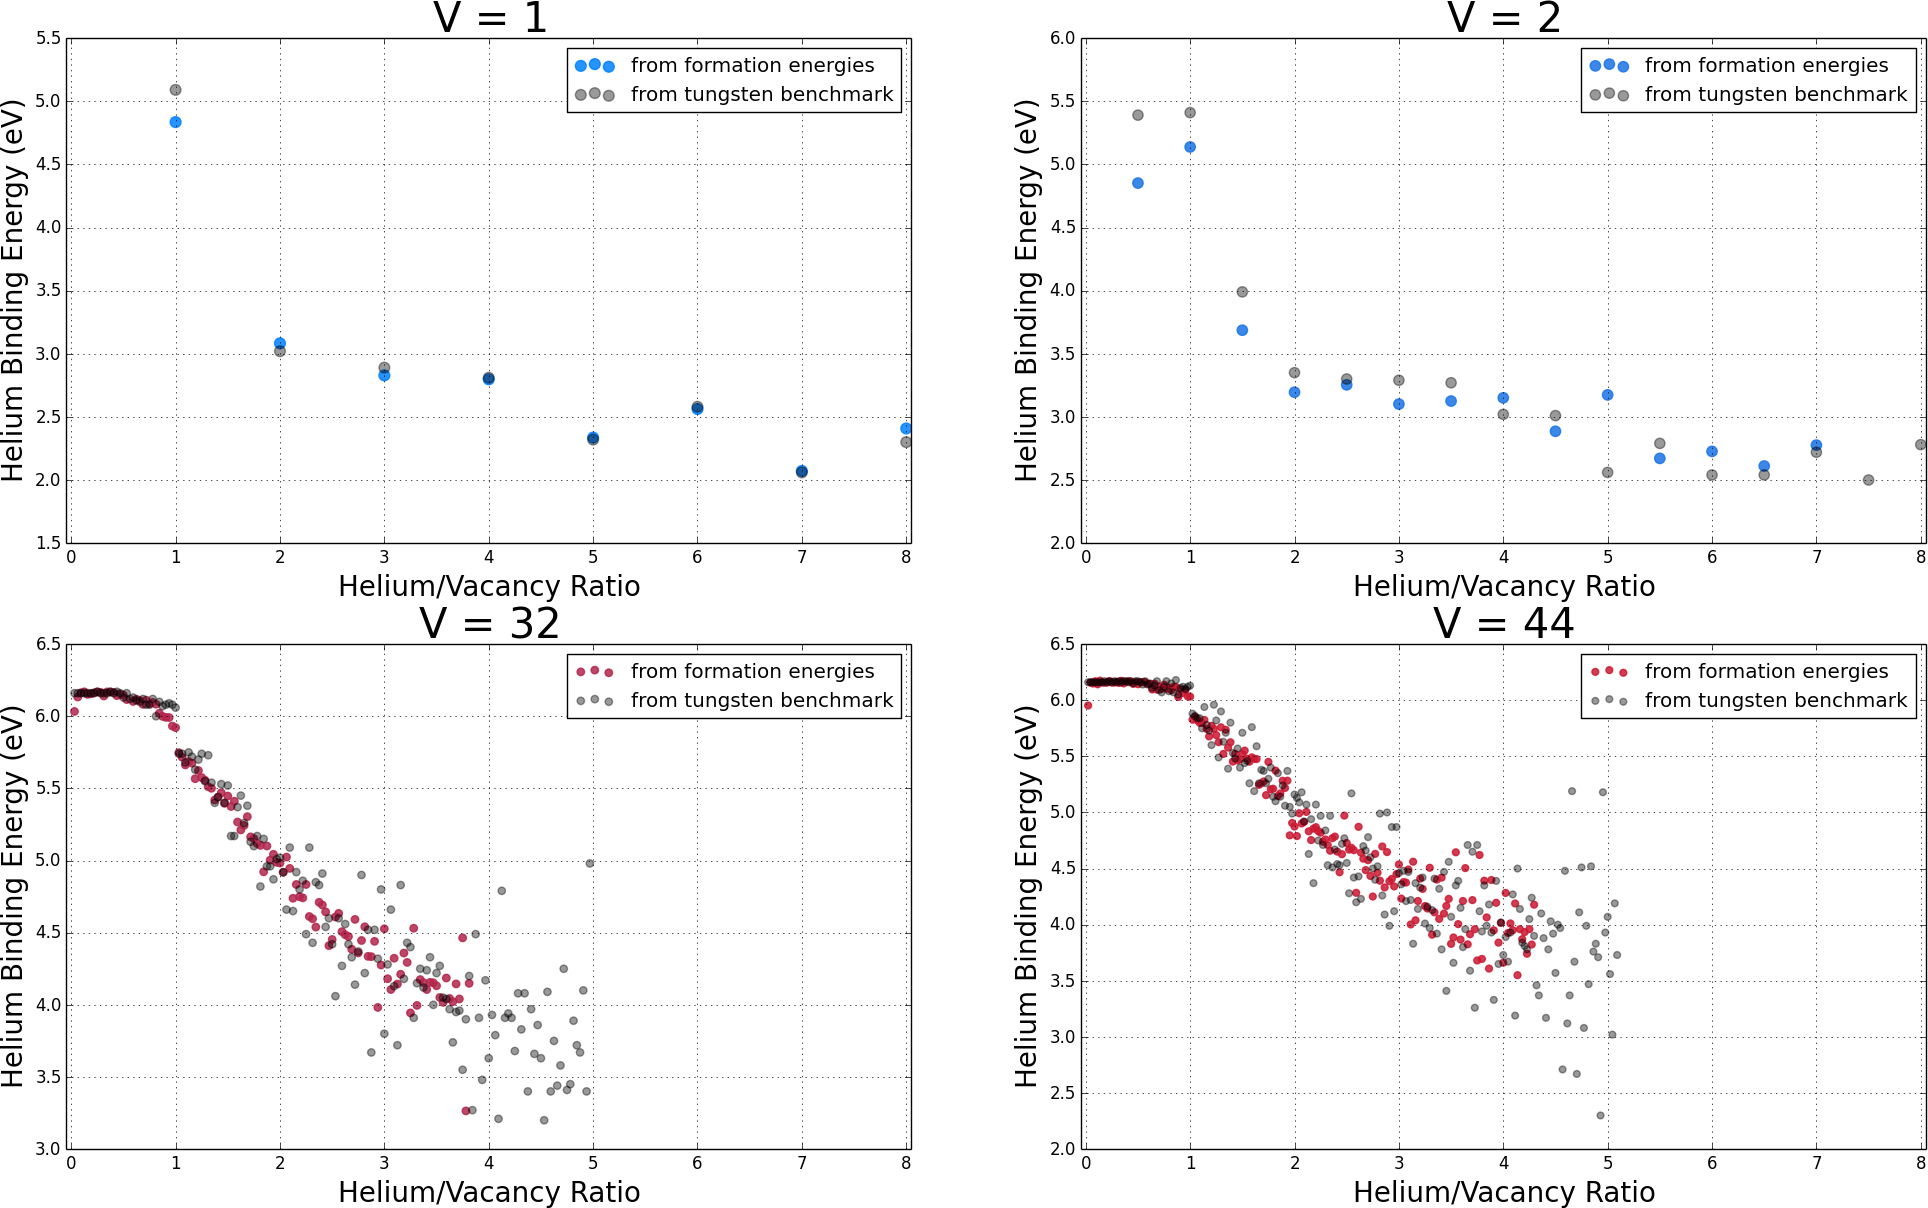
\includegraphics[width=0.9\textwidth]{bindingEnergiesComparison}
%     \end{figure}
% \end{frame}


\begin{frame}{Formation Energy Data}
  	\begin{columns}[onlytextwith]
    	\begin{column}{0.5\textwidth}
      		\begin{figure}
        		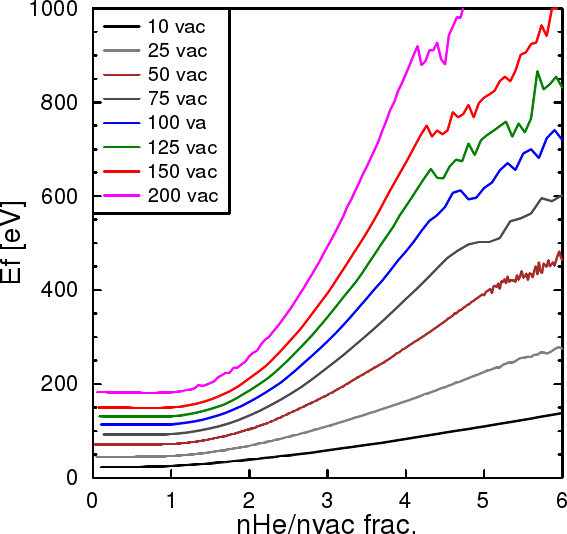
\includegraphics[width=\textwidth]{formationEnergyBrian}
      		\end{figure}
    	\end{column}  
    	\begin{column}{0.5\textwidth}
      		\begin{figure}
        		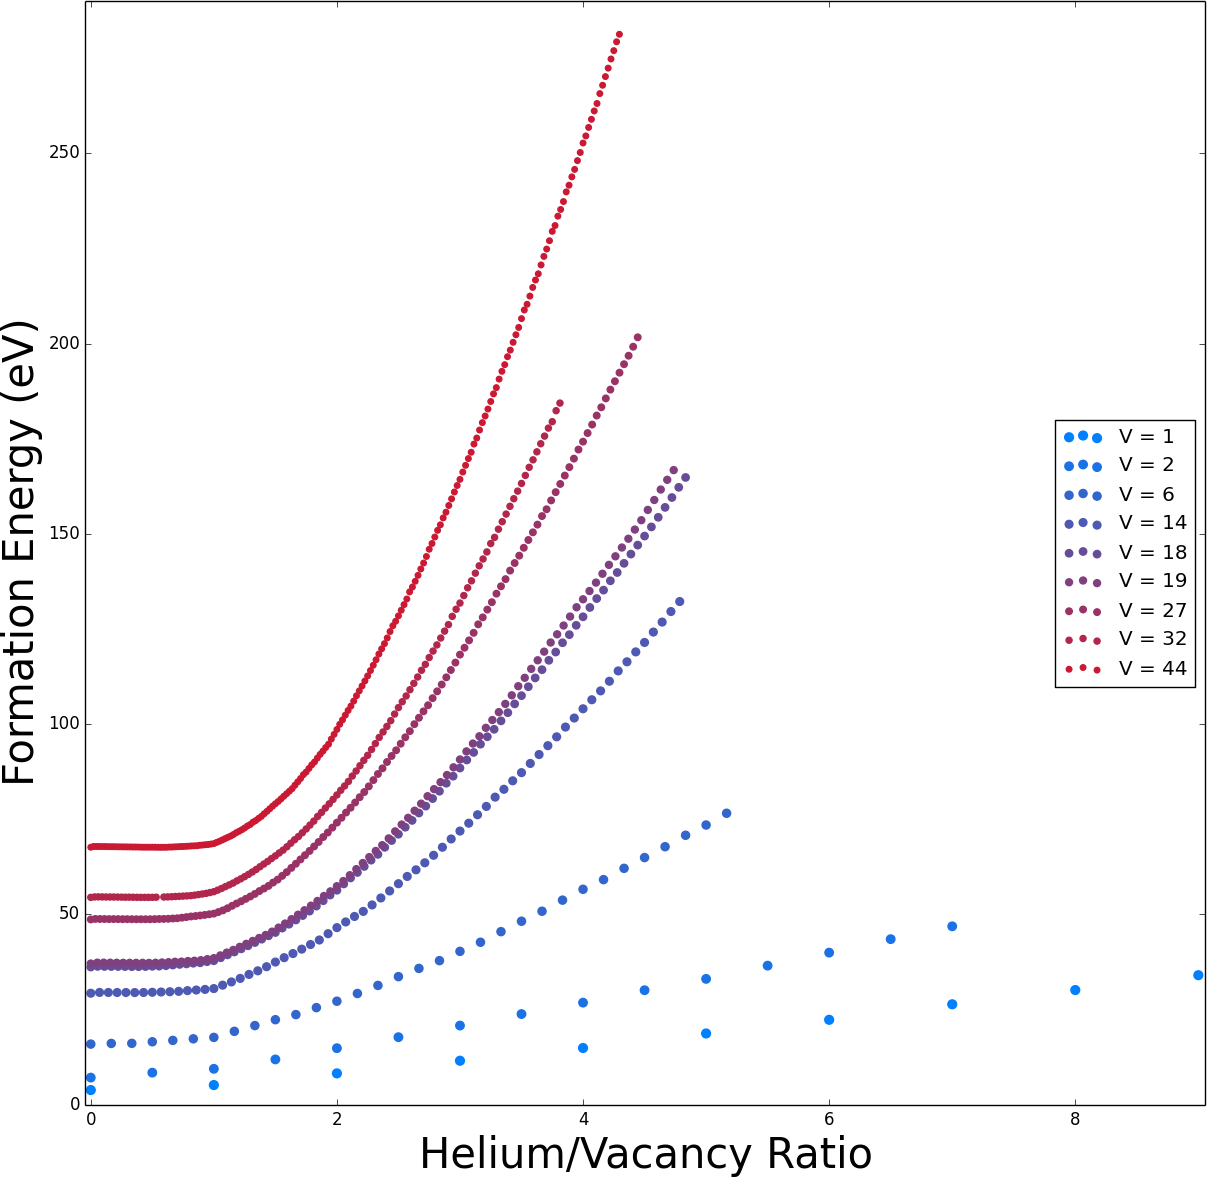
\includegraphics[width=0.9\textwidth]{formationEnergySophie}
      		\end{figure}
    	\end{column}
  	\end{columns}
\end{frame}

% \begin{frame}{From Juslin's Presentation}
% 	\begin{figure}
%         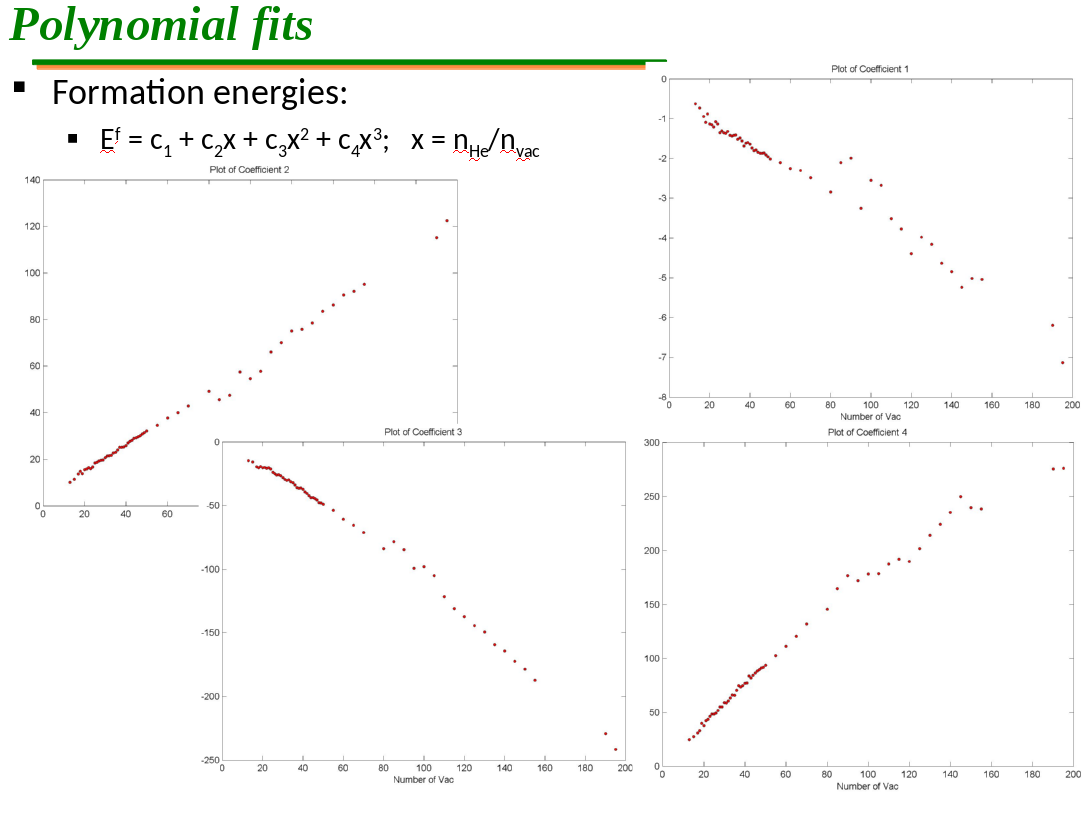
\includegraphics[width=0.9\textwidth]{fitsBrian}
%     \end{figure}
% \end{frame}
% 
% 
% \begin{frame}{Fitting Methods}
% 	\large
%     \begin{itemize}
%       	\item[$\blacktriangleright$] Piecewise $2$D polynomials fit with a
%       	separation arround He/V~$=1$ where the order of the lower and higher
%       	parts can be chosen independently \newline
%       	\item[$\blacktriangleright$] Two-step $1$D polynomials fits:
%     	\begin{itemize}
%       		\item[-] Use only polynomials
%       		\item[-] Piecewise fit first on the formation
%       		energies as a function of He/V with a separation arround He/V~$=1$
%       		\item[-] Fit then the parameters of those fits as a
%       		function of V
%       		\item[-] Each fit orders ($4$ in total) and the
%       		separation can be changed
%     	\end{itemize}
%     \end{itemize}
% \end{frame}
% 
% \begin{frame}{Example of Two-Step fit:}
% 	Order $1$ and order $3$ polynomials for V~$= 1$ 
% 	\begin{figure}
%         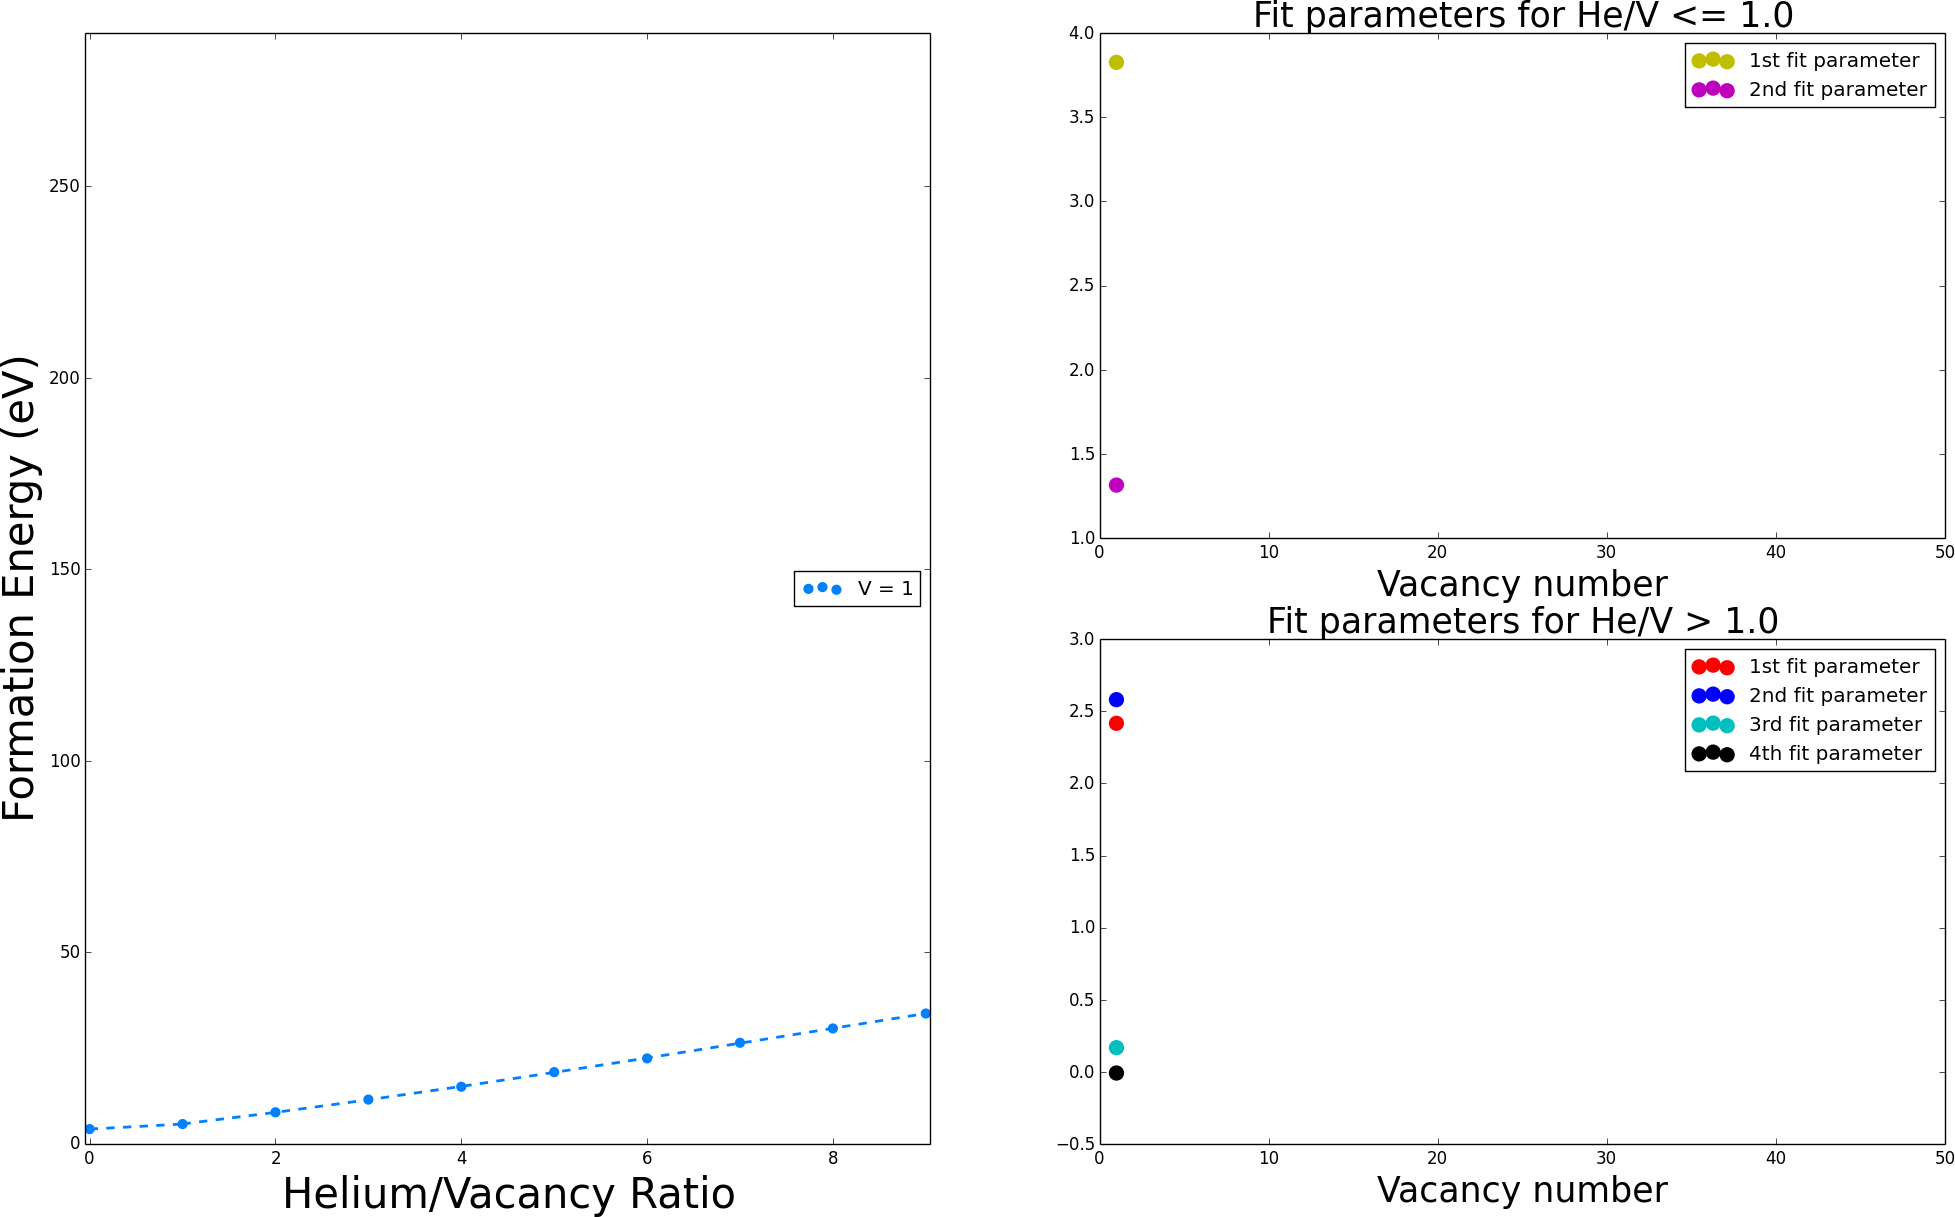
\includegraphics[width=0.95\textwidth]{fit1DS1}
%     \end{figure}
% \end{frame}
% 
% \begin{frame}{Example of Two-Step fit:}
% 	Order $1$ and order $3$ polynomials for V~$= 2$
% 	\begin{figure}
%         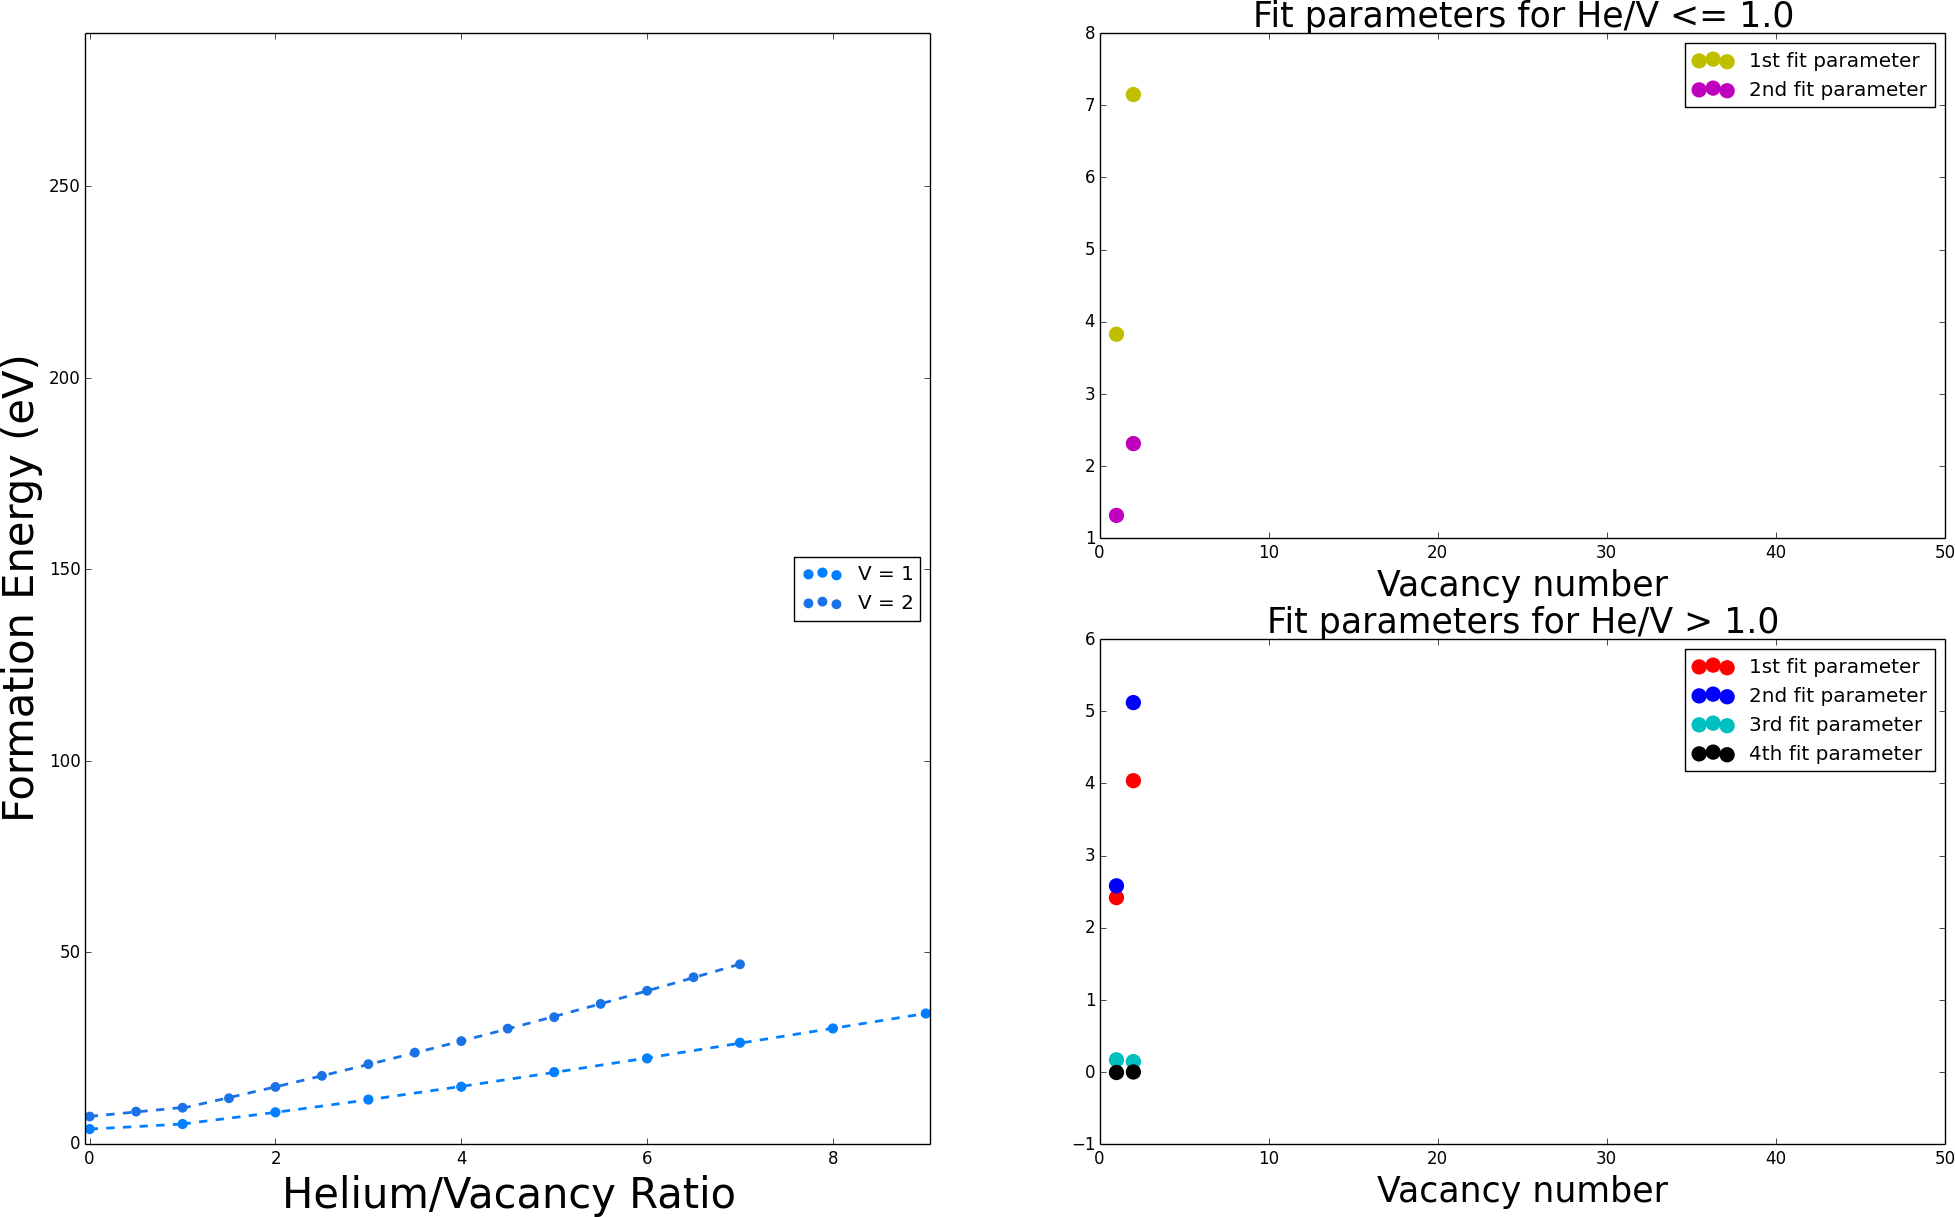
\includegraphics[width=0.95\textwidth]{fit1DS2}
%     \end{figure}
% \end{frame}
% 
% \begin{frame}{Example of Two-Step fit:}
% 	Order $1$ and order $3$ polynomials for all V
% 	\begin{figure}
%         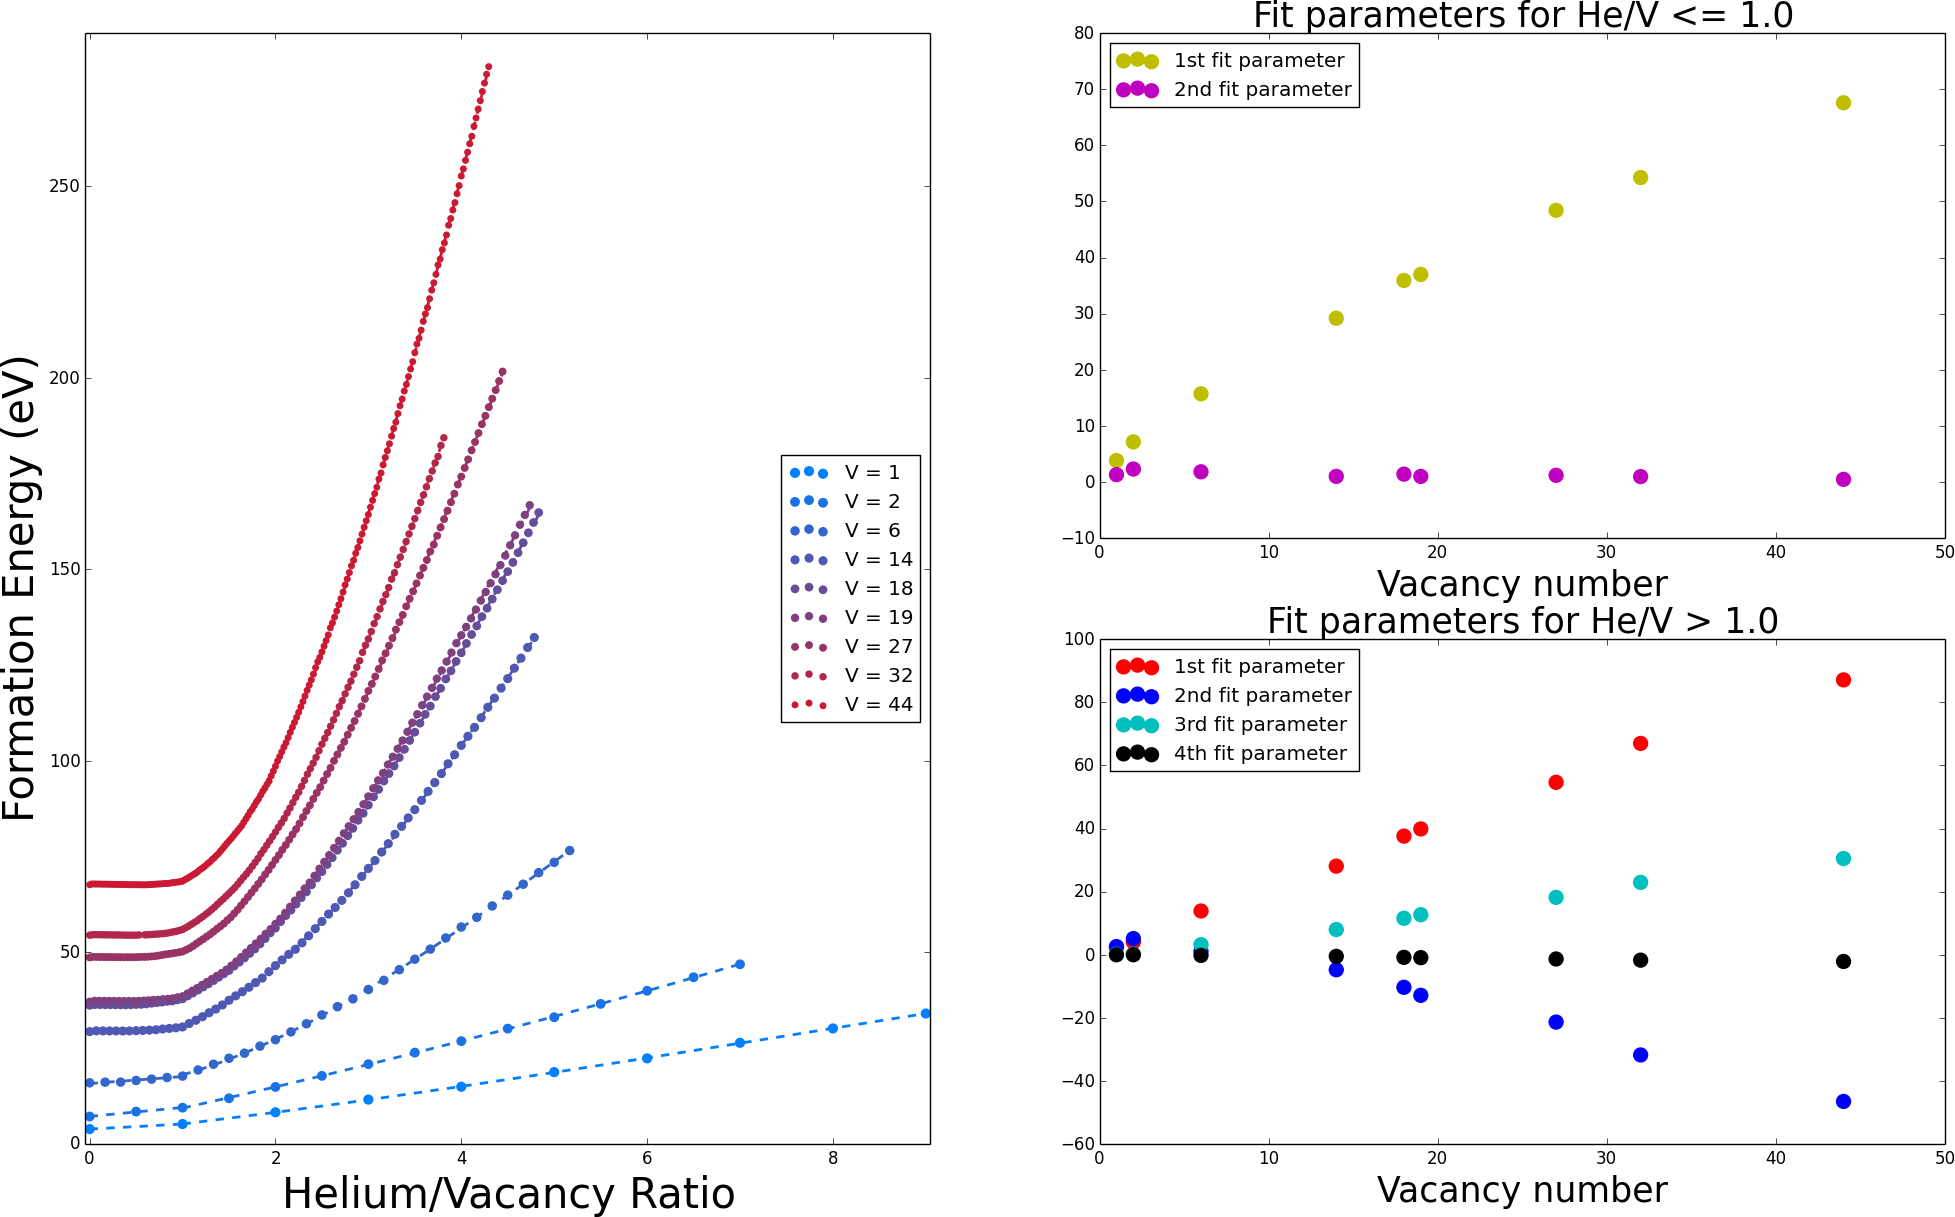
\includegraphics[width=0.95\textwidth]{fit1DS3}
%     \end{figure}
% \end{frame}
% 
% \begin{frame}{Example of Two-Step fit:}
% 	Fit the parameters with order $3$ polynomials
% 	\begin{figure}
%         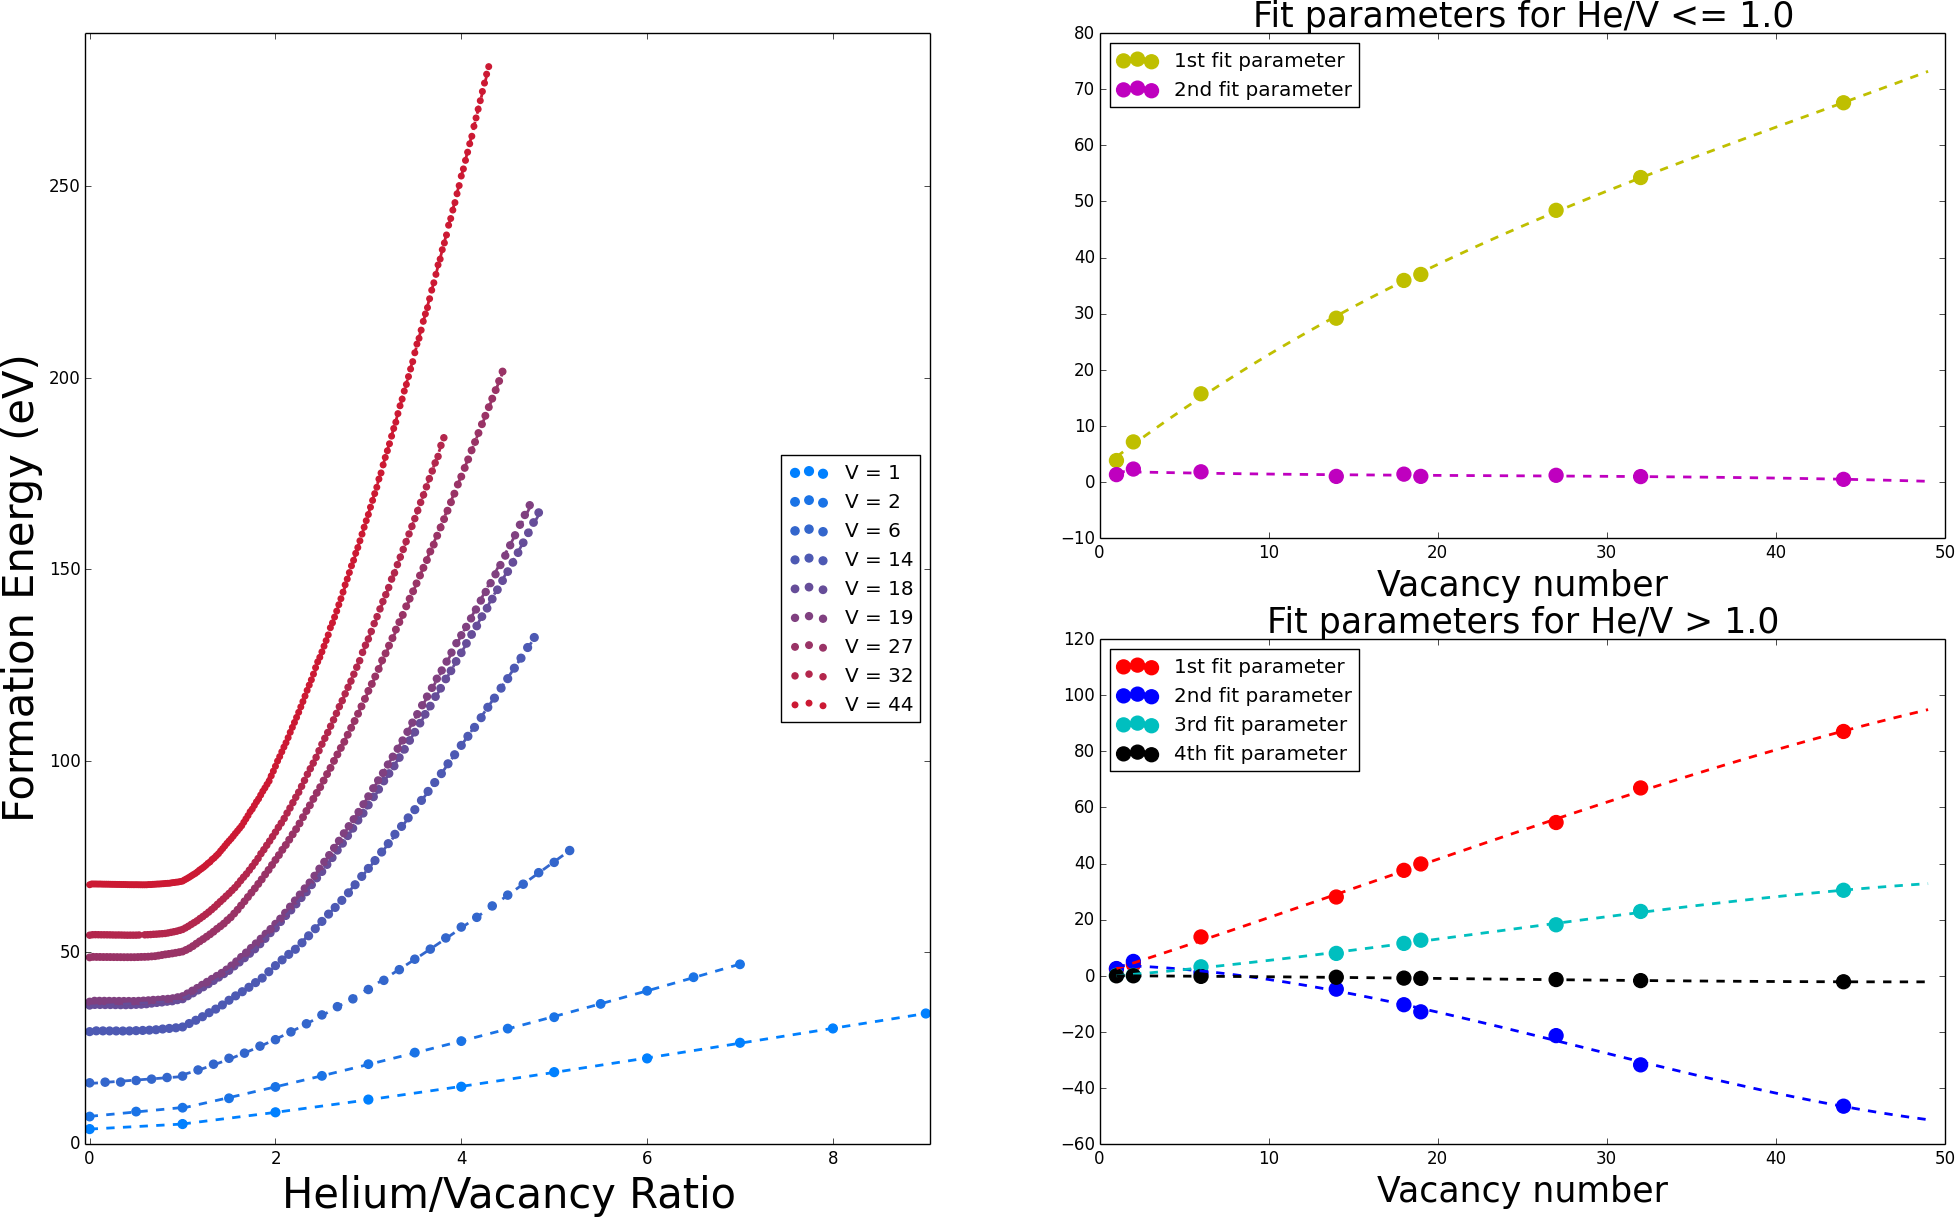
\includegraphics[width=0.95\textwidth]{fit1DS4}
%     \end{figure}
% \end{frame}
% 
% \begin{frame}{Example of Two-Step fit:}
% 	Use the obtained parameters to define a $2$D function
% 	\begin{figure}
%         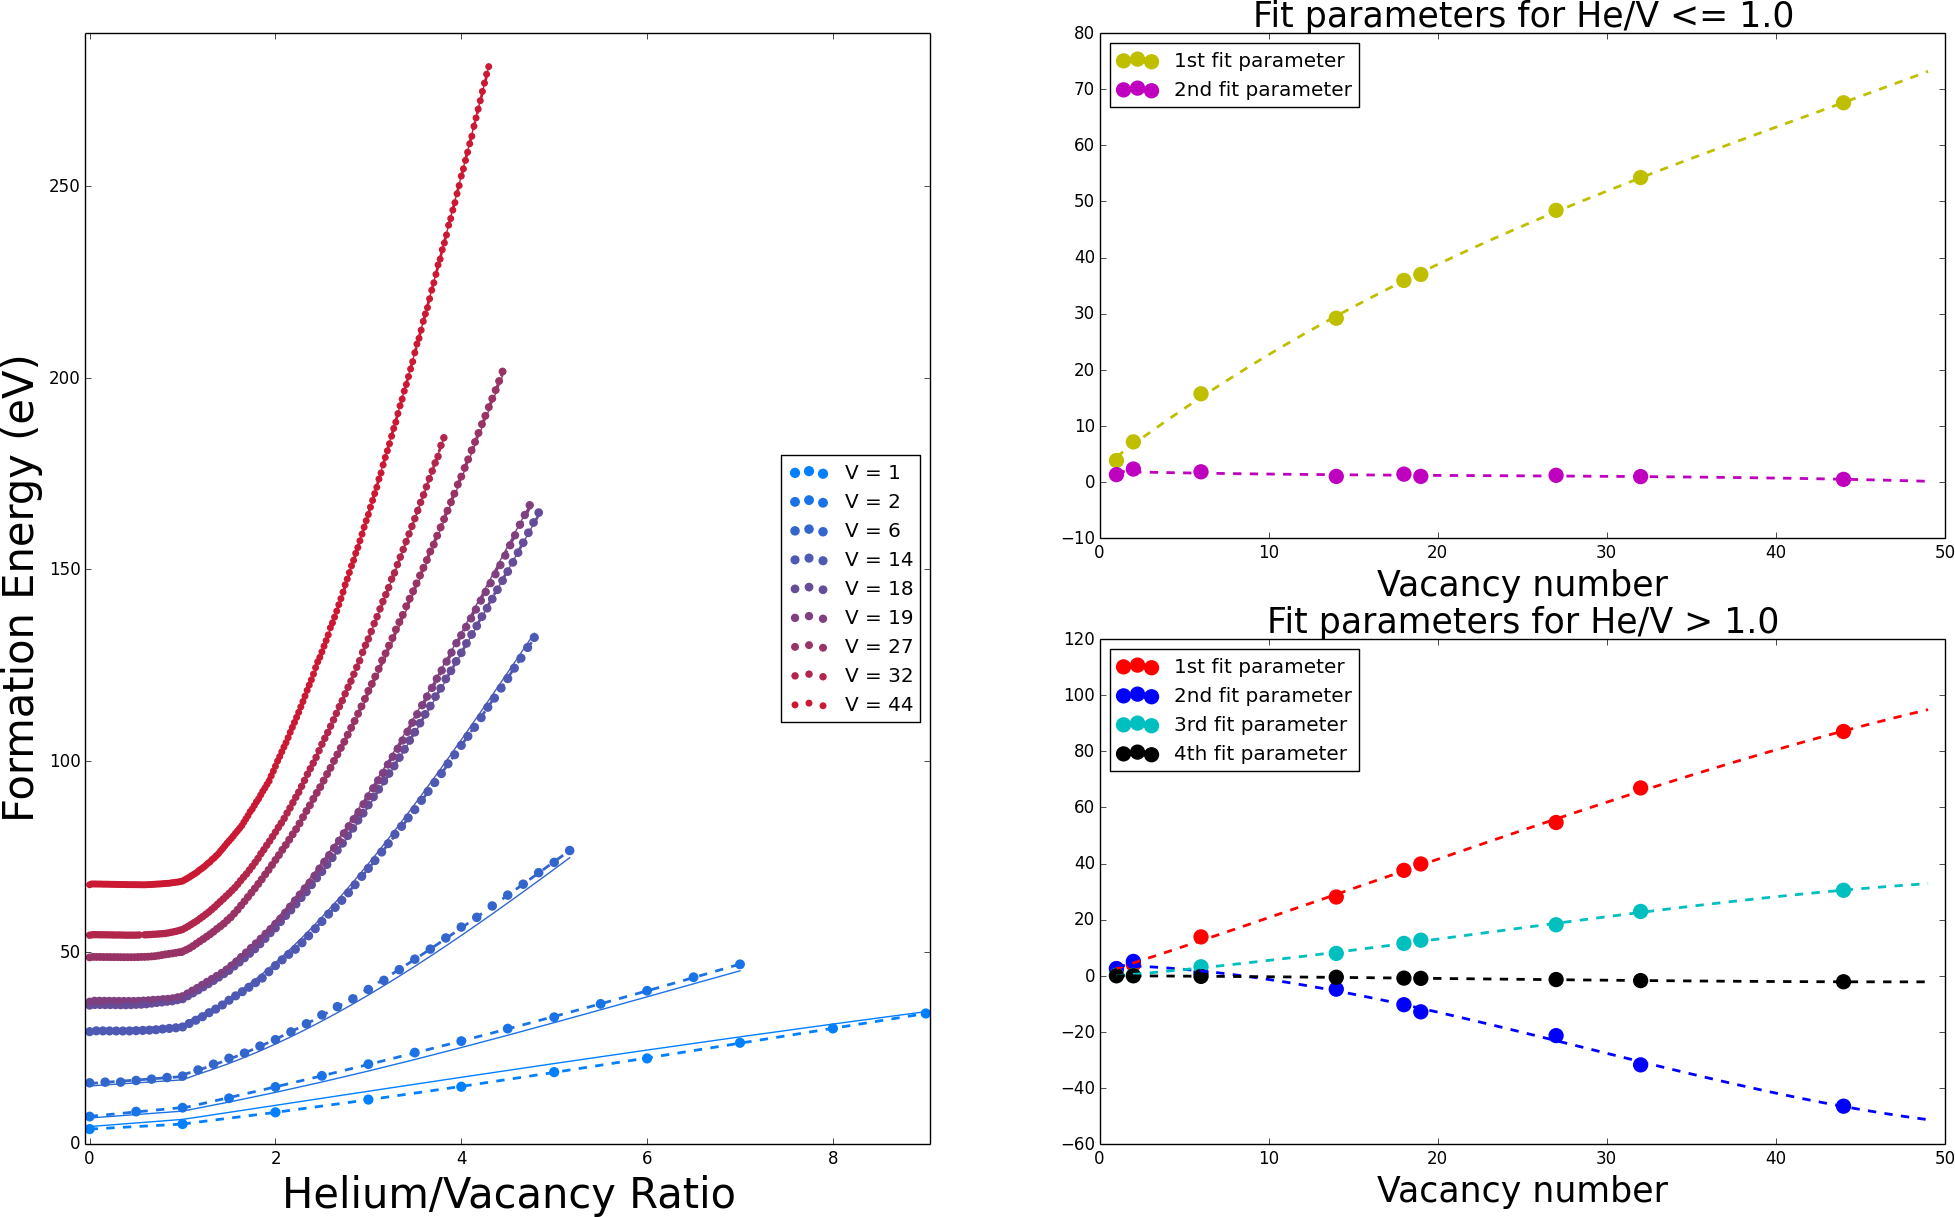
\includegraphics[width=0.95\textwidth]{fit1DS5}
%     \end{figure}
% \end{frame}
% 
% \begin{frame}{Example of Two-Step fit $(1., 1, 3, 3, 3)$}
% 	Result:
% 	\begin{figure}
%         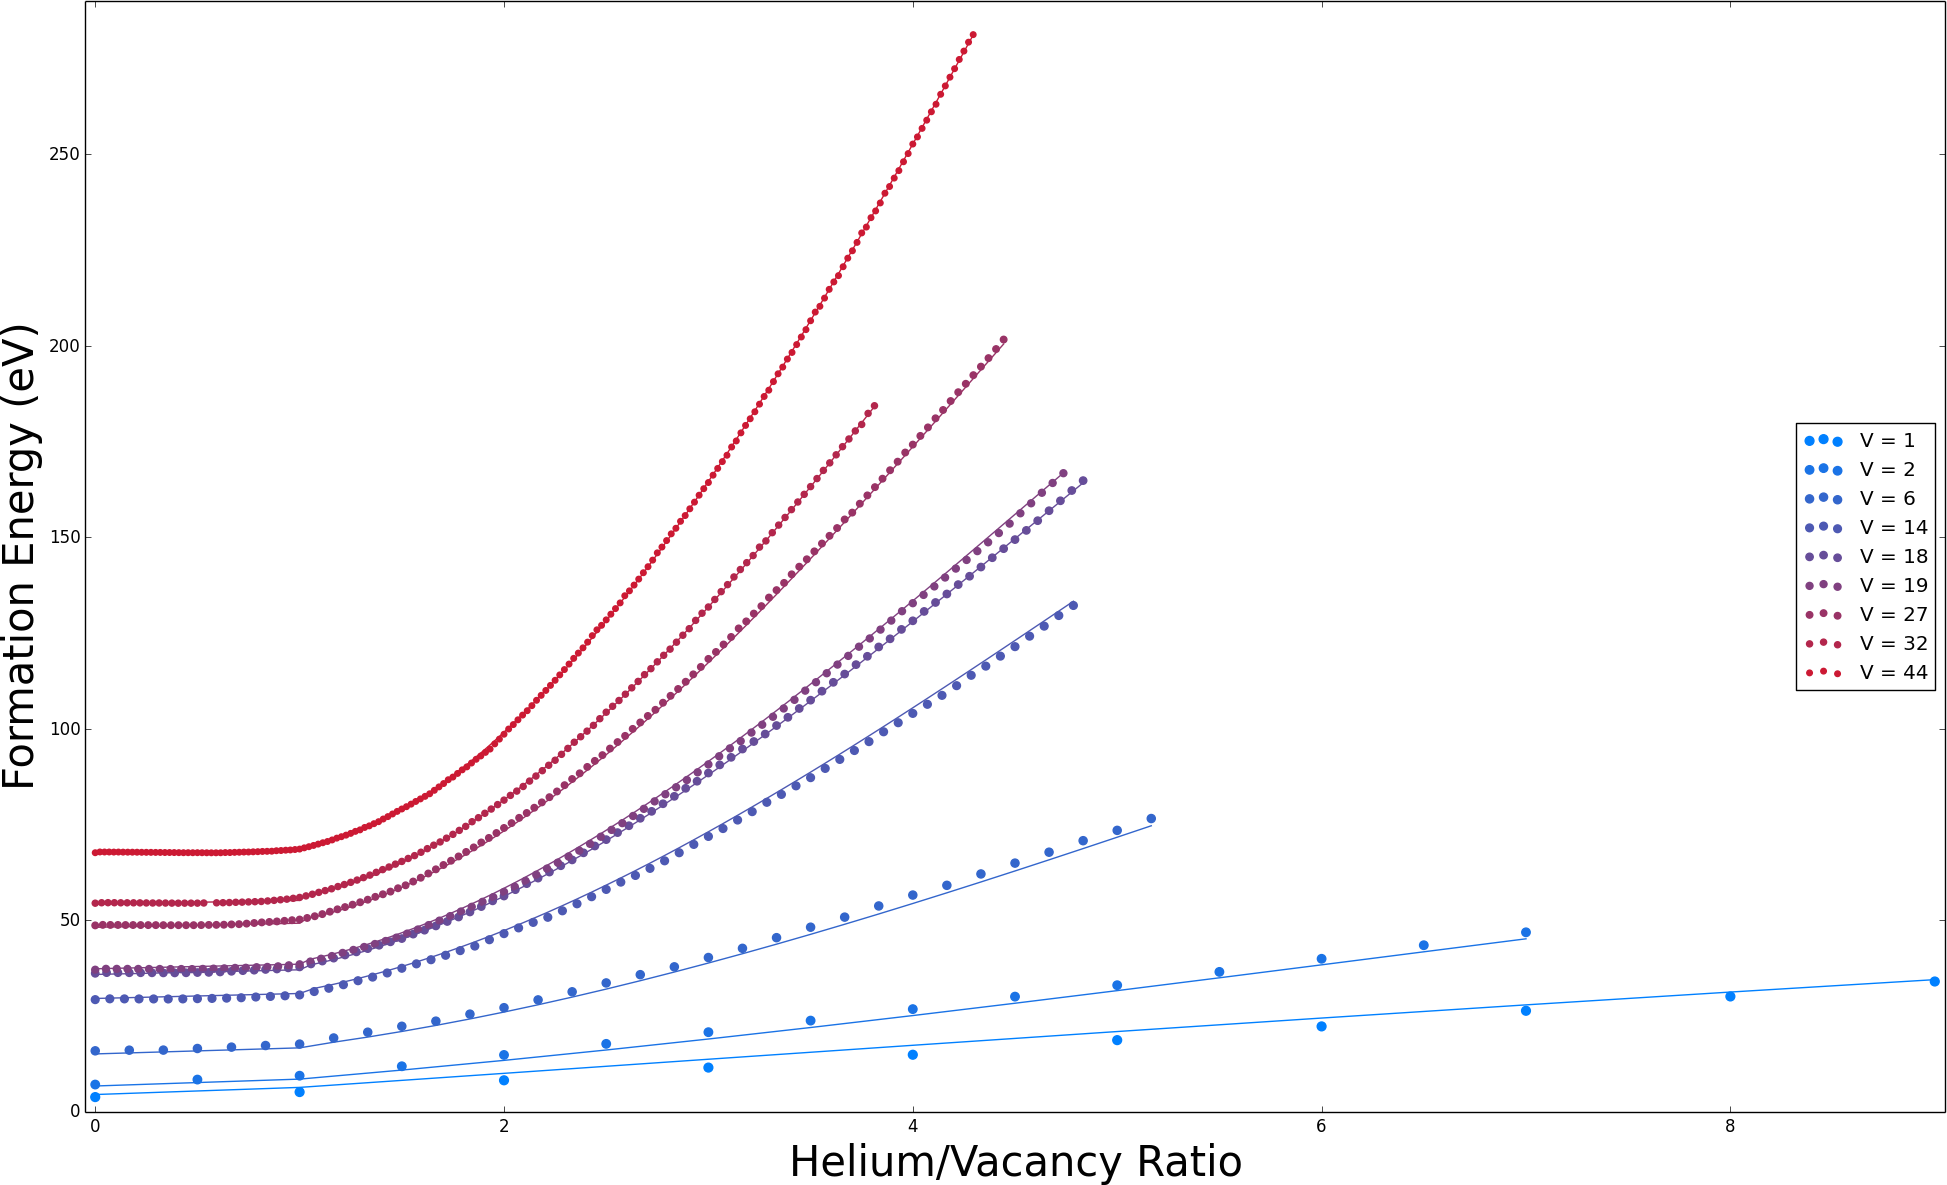
\includegraphics[width=0.95\textwidth]{formationFit1D_13331}
%     \end{figure}
% \end{frame}
% 
% \begin{frame}{Selection Criteria}
% 	\large
%     \begin{itemize}
%       	\item[$\blacktriangleright$] The closest to the formation energies.
%       	\newline
%       	\item[$\blacktriangleright$] Polynomial orders lower or equal to $3$.
%     \end{itemize}
% \end{frame}
% 
% \begin{frame}{Best $2$D fit $(1.1, 3, 3)$}
% 	\begin{figure}
%         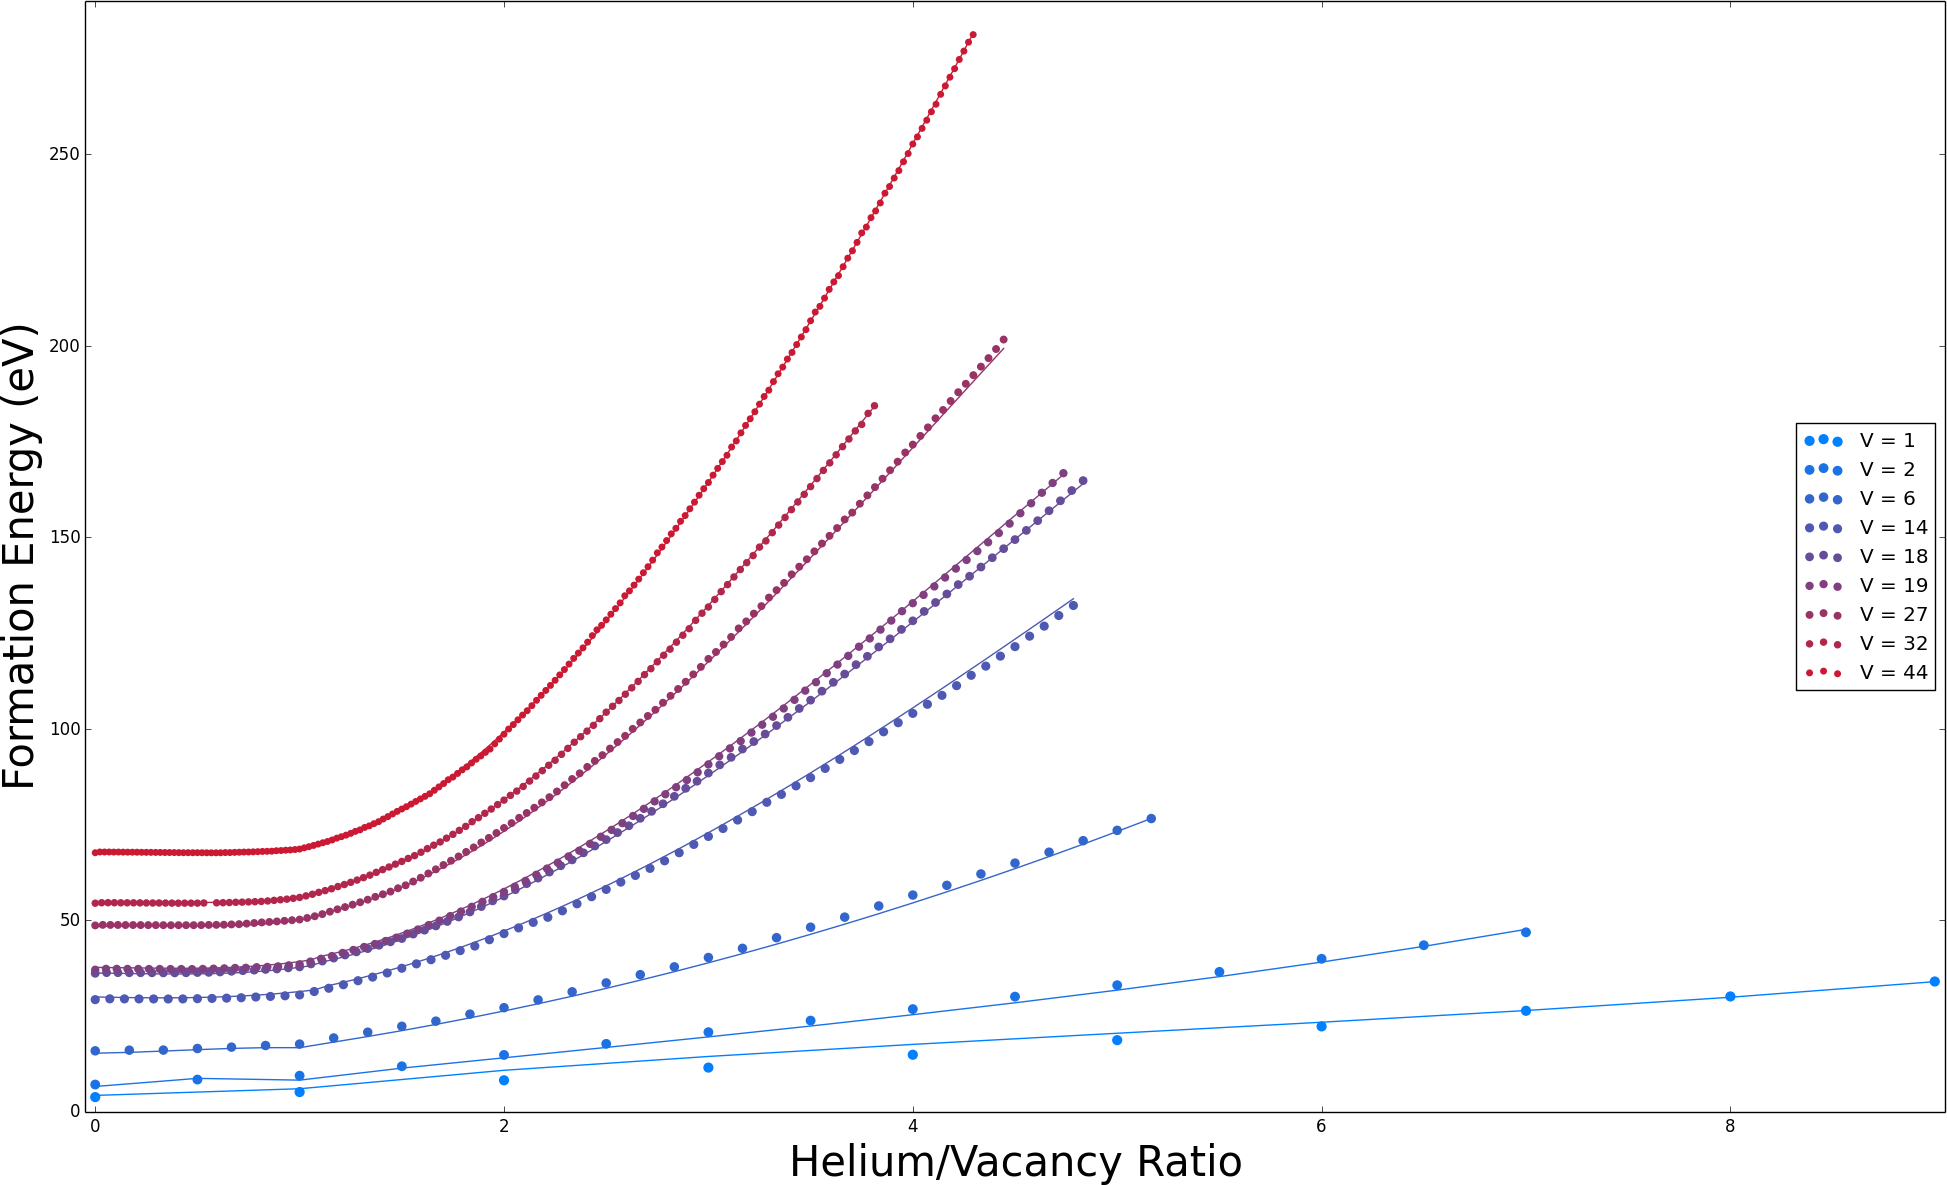
\includegraphics[width=0.95\textwidth]{formationFit2D_3311}
%     \end{figure}
% \end{frame}
% 
% \begin{frame}{Best Two-Step fit $(1., 2, 3, 3, 3)$}
% 	\begin{figure}
%         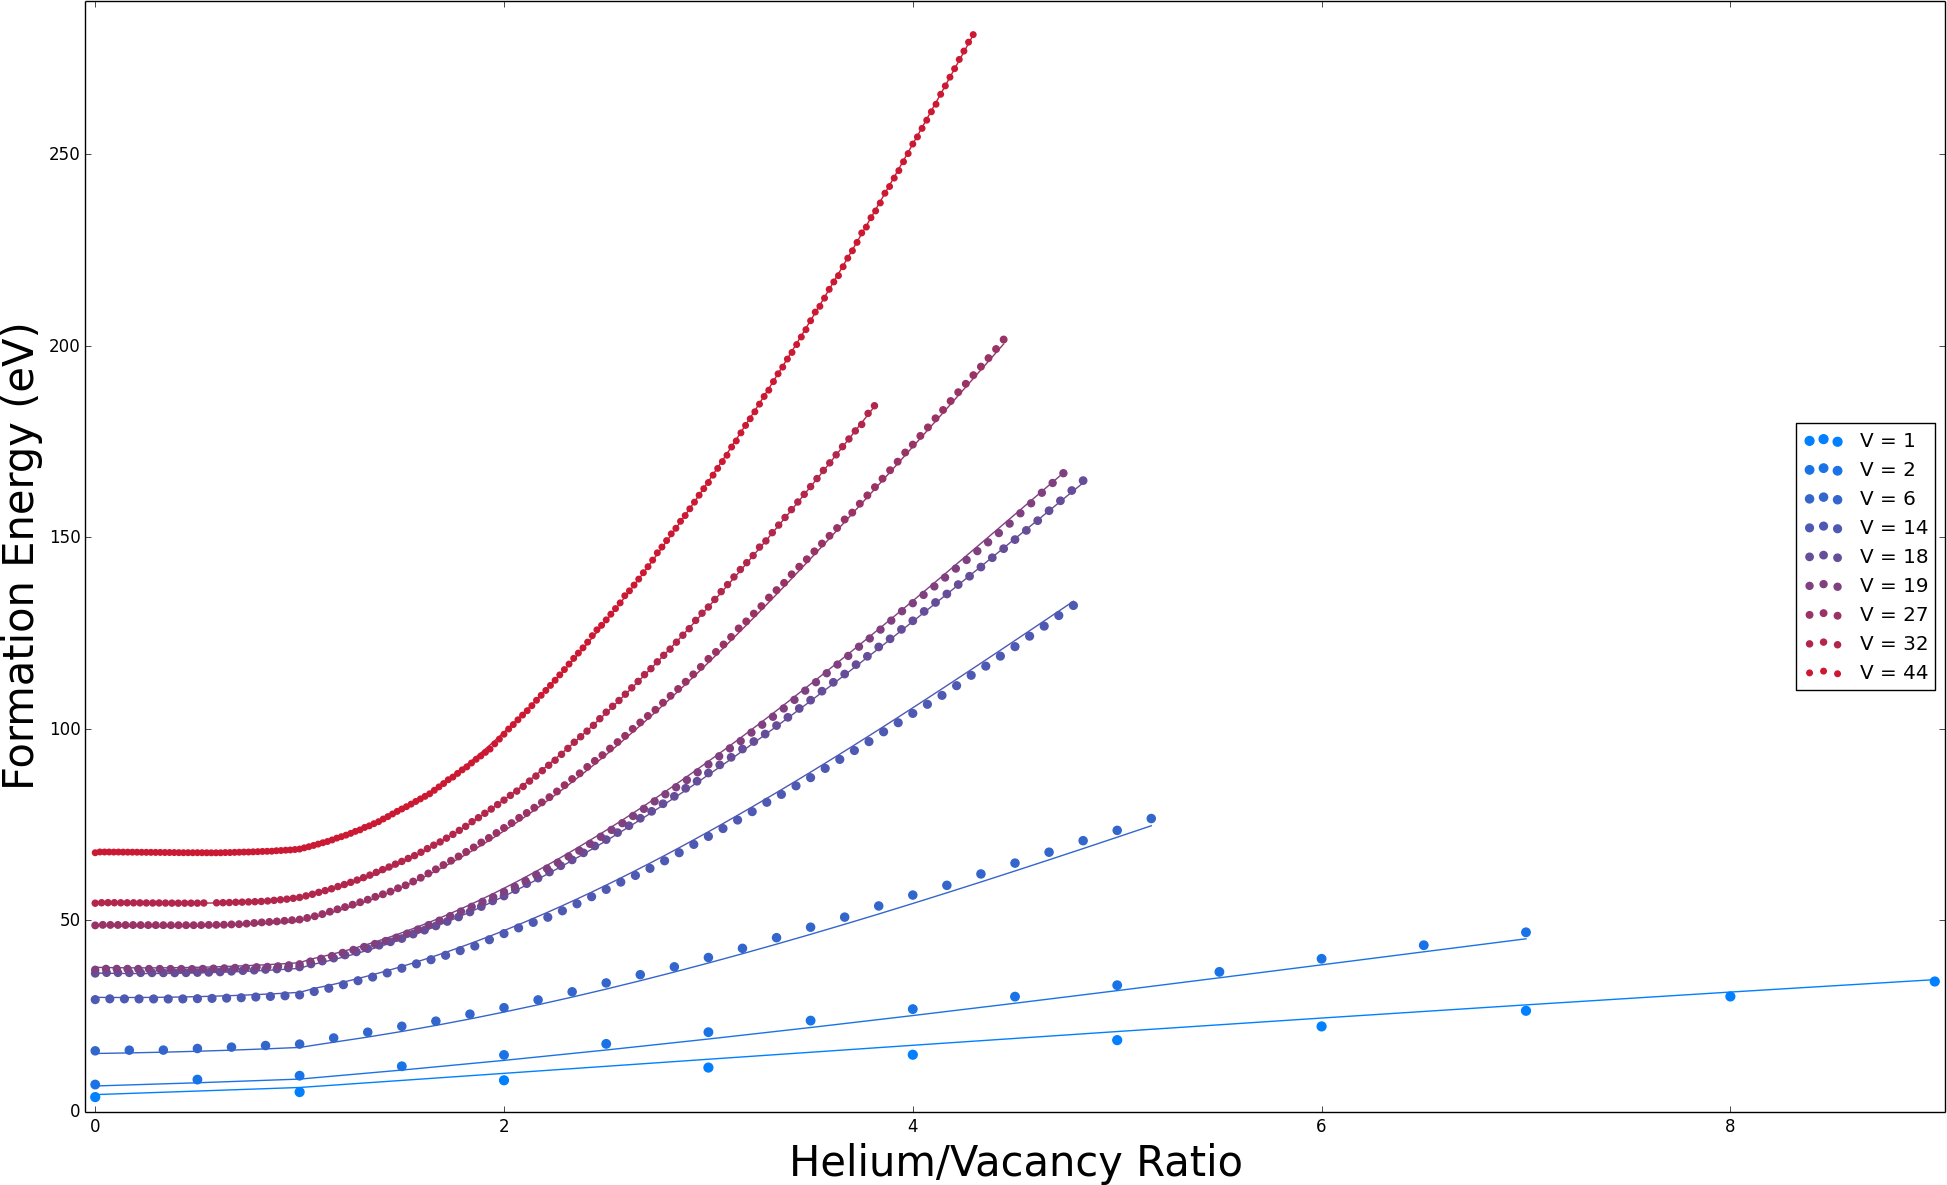
\includegraphics[width=0.95\textwidth]{formationFit1D_23331}
%     \end{figure}
% \end{frame}
% 
% \begin{frame}{Binding Energies, $2$D fit $(1.1, 3, 3)$}
% 	\begin{figure}
%         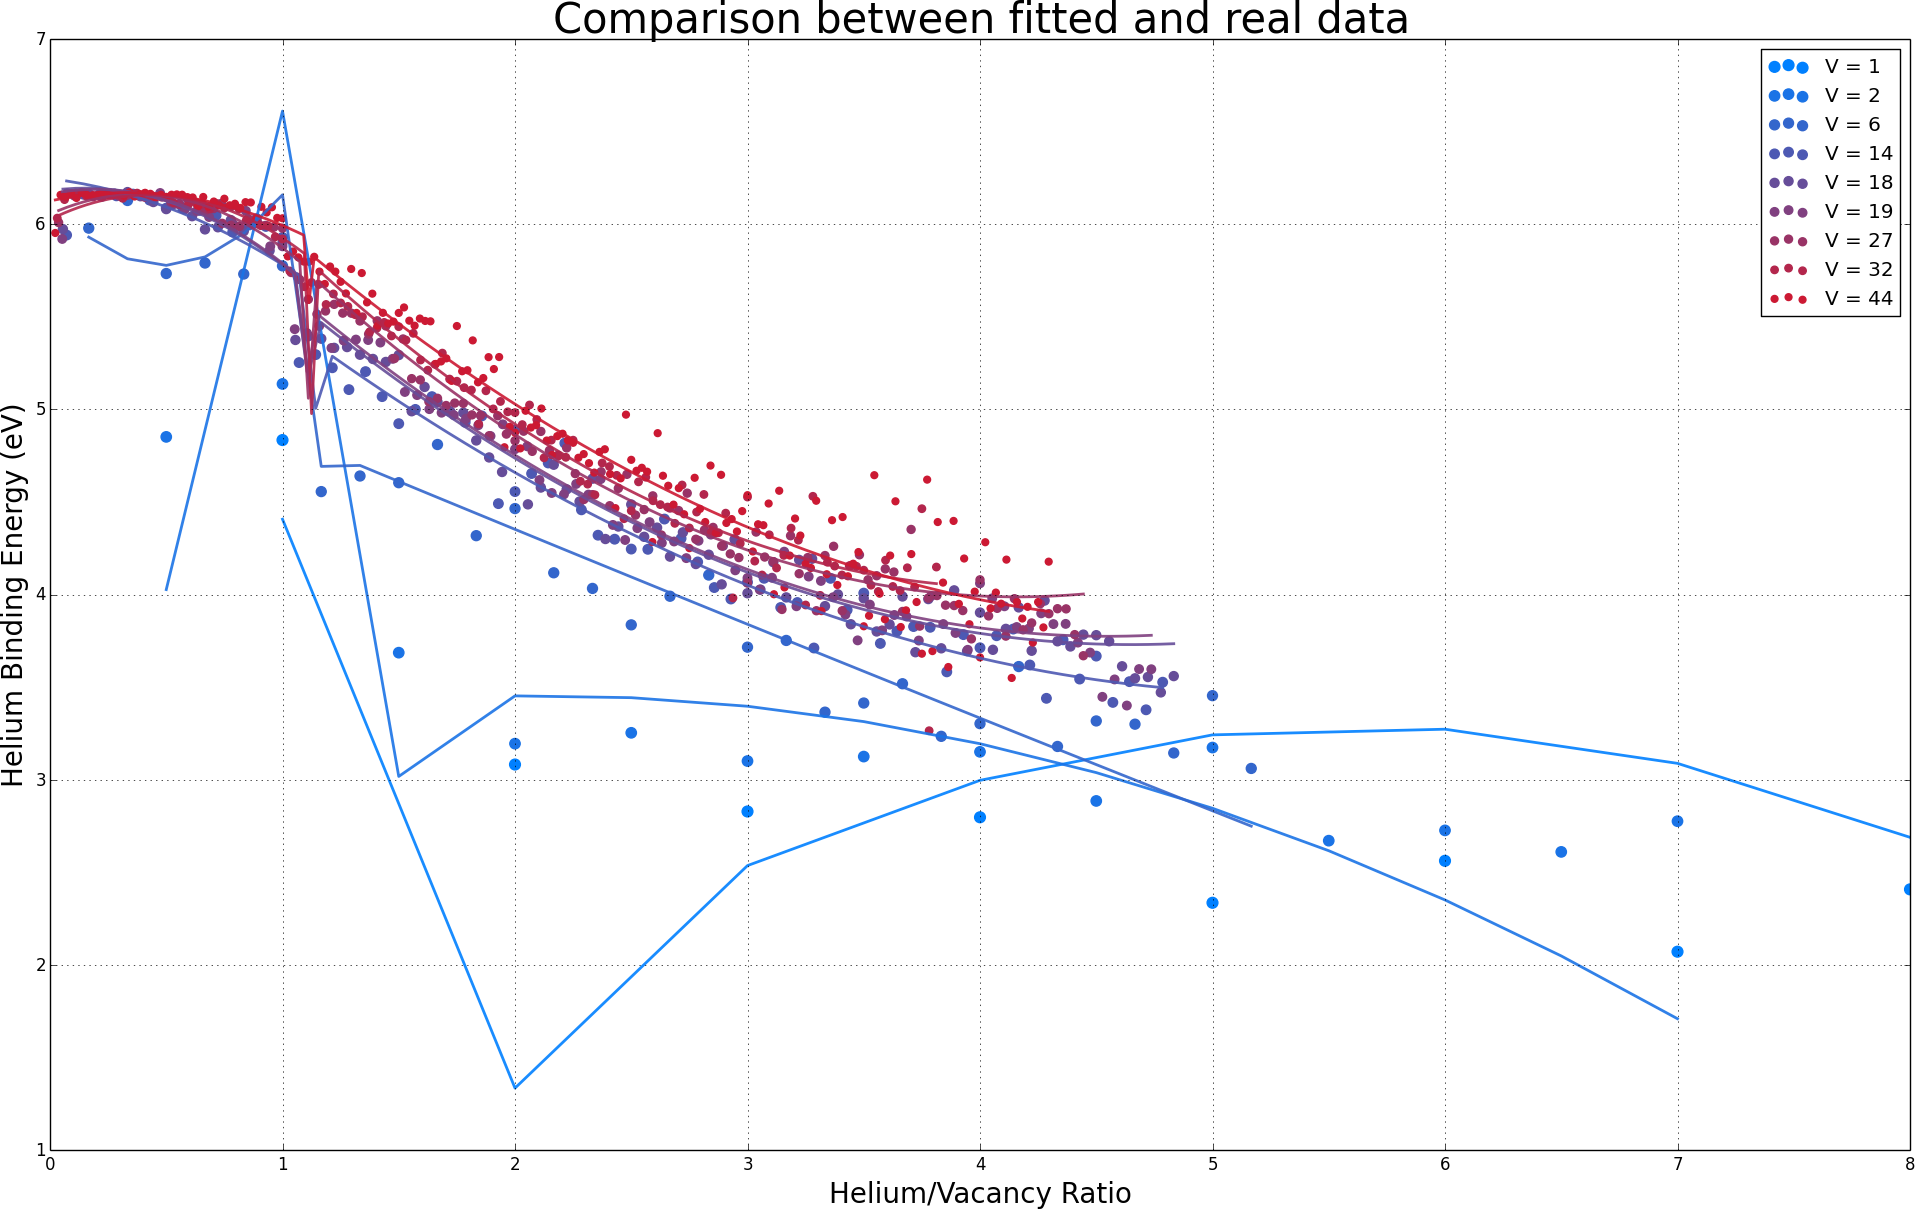
\includegraphics[width=0.95\textwidth]{bindingFit2D_3311}
%     \end{figure}
% \end{frame}
% 
% \begin{frame}{Binding Energies, Two-Step fit $(1., 2, 3, 3, 3)$}
% 	\begin{figure}
%         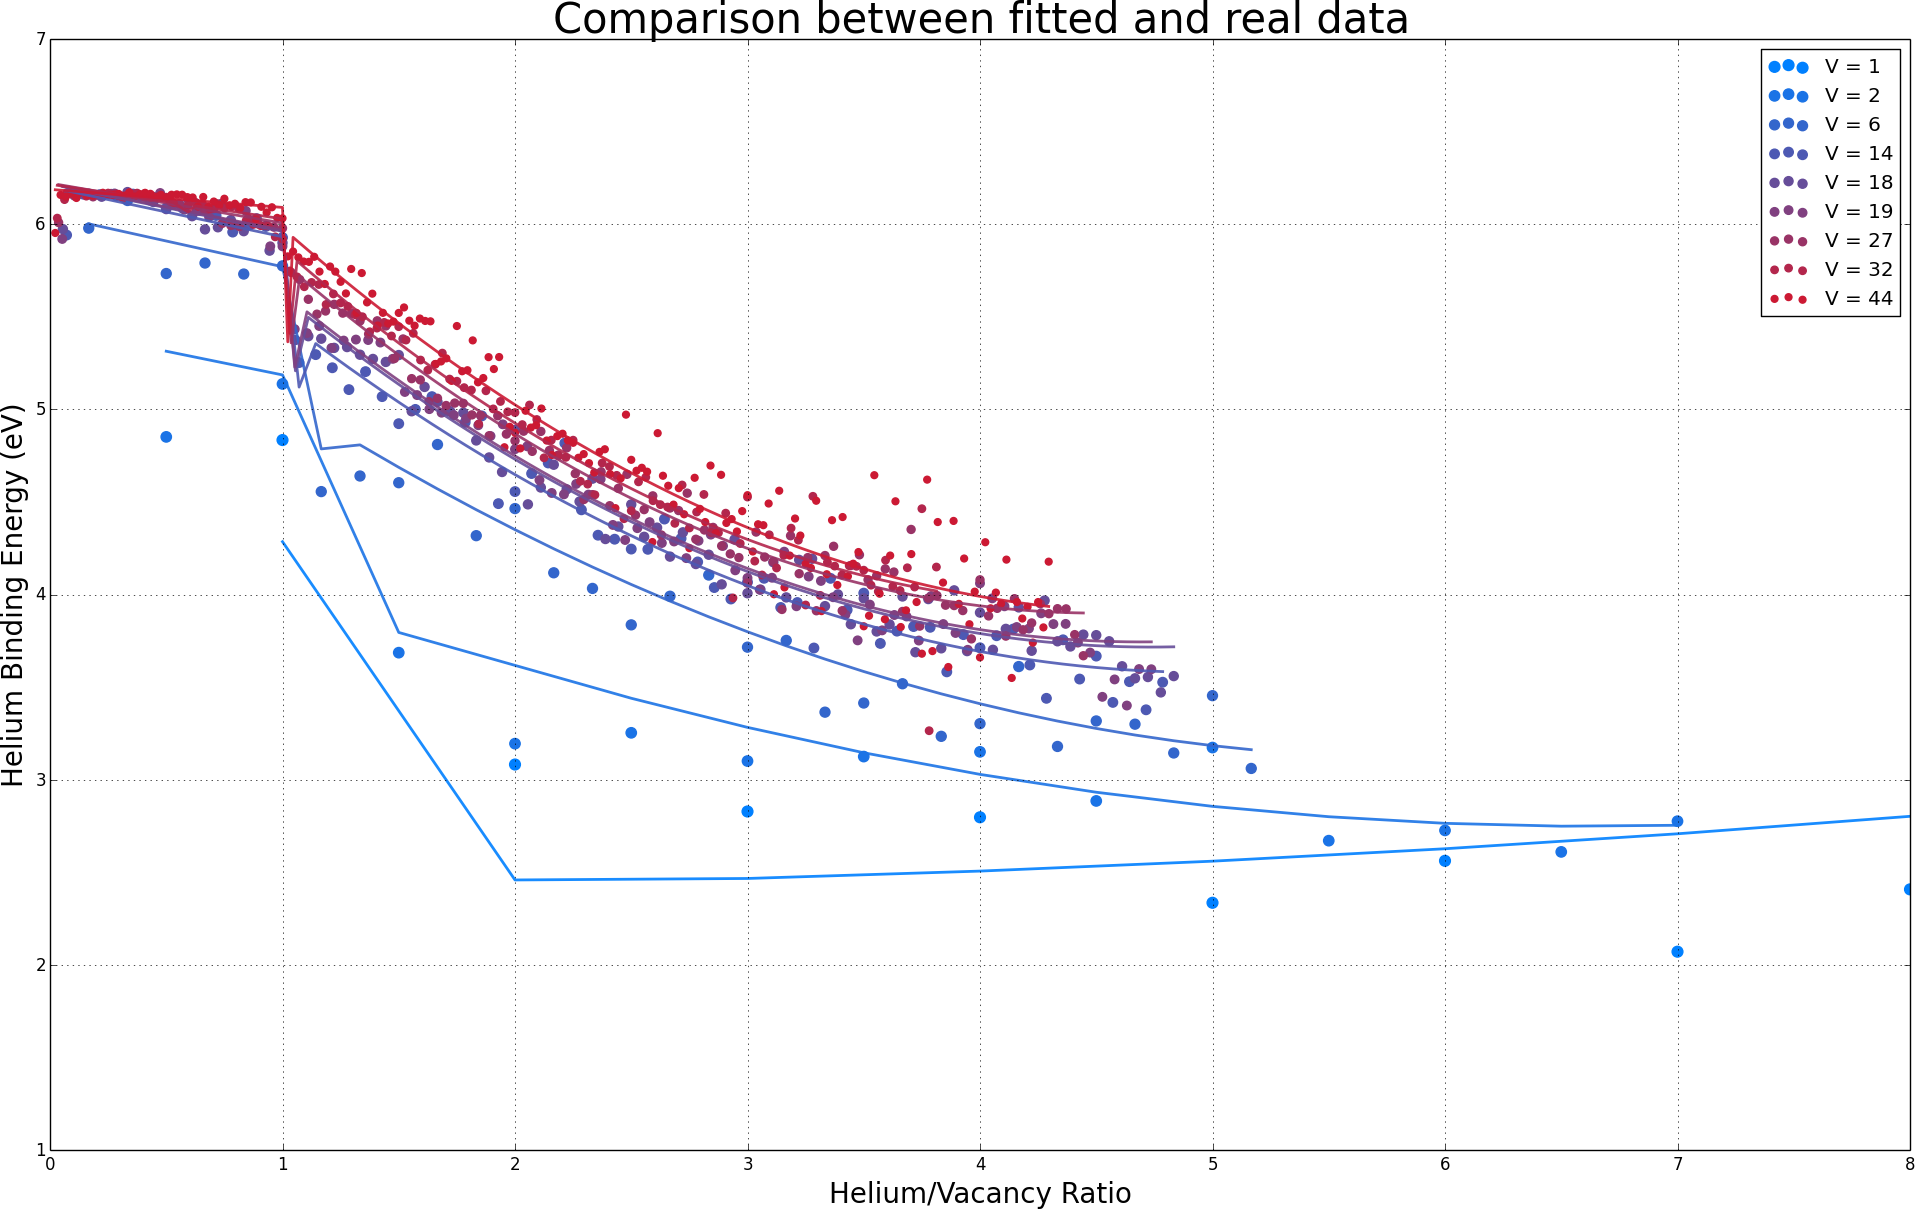
\includegraphics[width=0.95\textwidth]{bindingFit1D_23331}
%     \end{figure}
% \end{frame}
% 
% \begin{frame}{Confidence Interval of the Fit}
% 	\large
% 	Compare the given formation energies to the fitted ones:
%     \begin{itemize}
%       	\item[$\blacktriangleright$] compute the distance between them for each
%       	vacancy number
%       	\item[$\blacktriangleright$] plot it in a histogram and fit it with a
%       	normal distribution \newline
%     \end{itemize}
%     \normalsize
%     Example for V~$=32$: 
% 	\begin{figure}
%         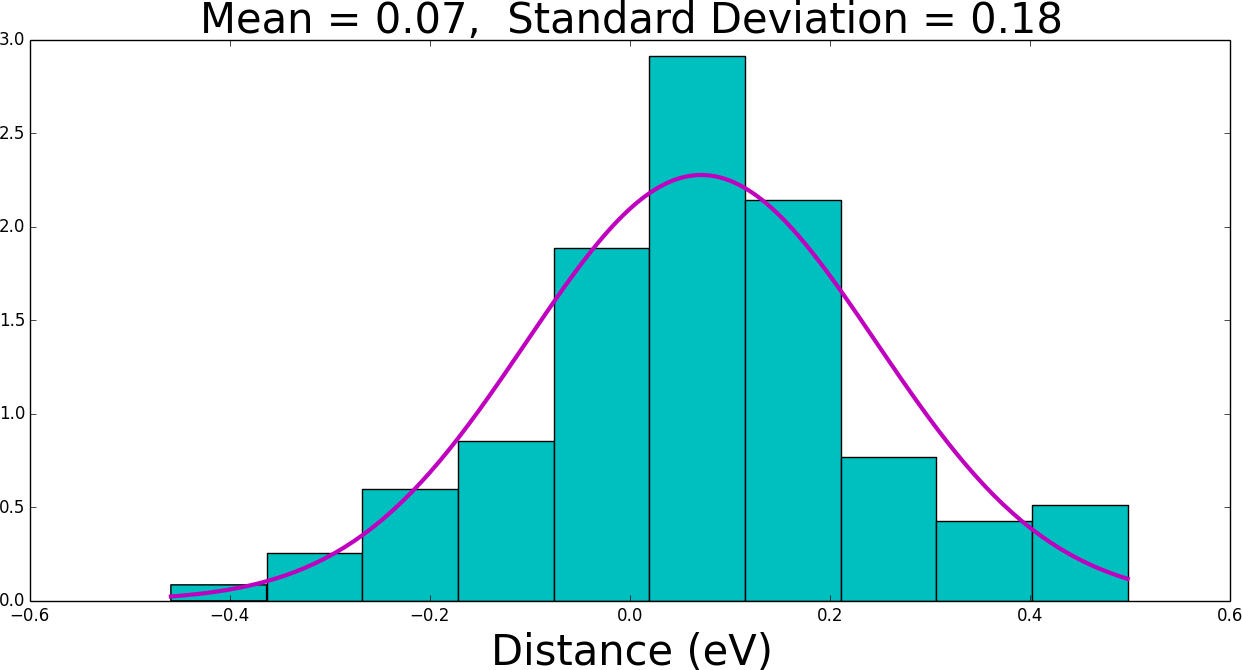
\includegraphics[width=0.6\textwidth]{confidenceInterval32}
%     \end{figure}
% \end{frame}
% 
% \begin{frame}{Confidence Interval of the Fit}
% 	Summary for all vacancy numbers:
% 	\begin{figure}
%         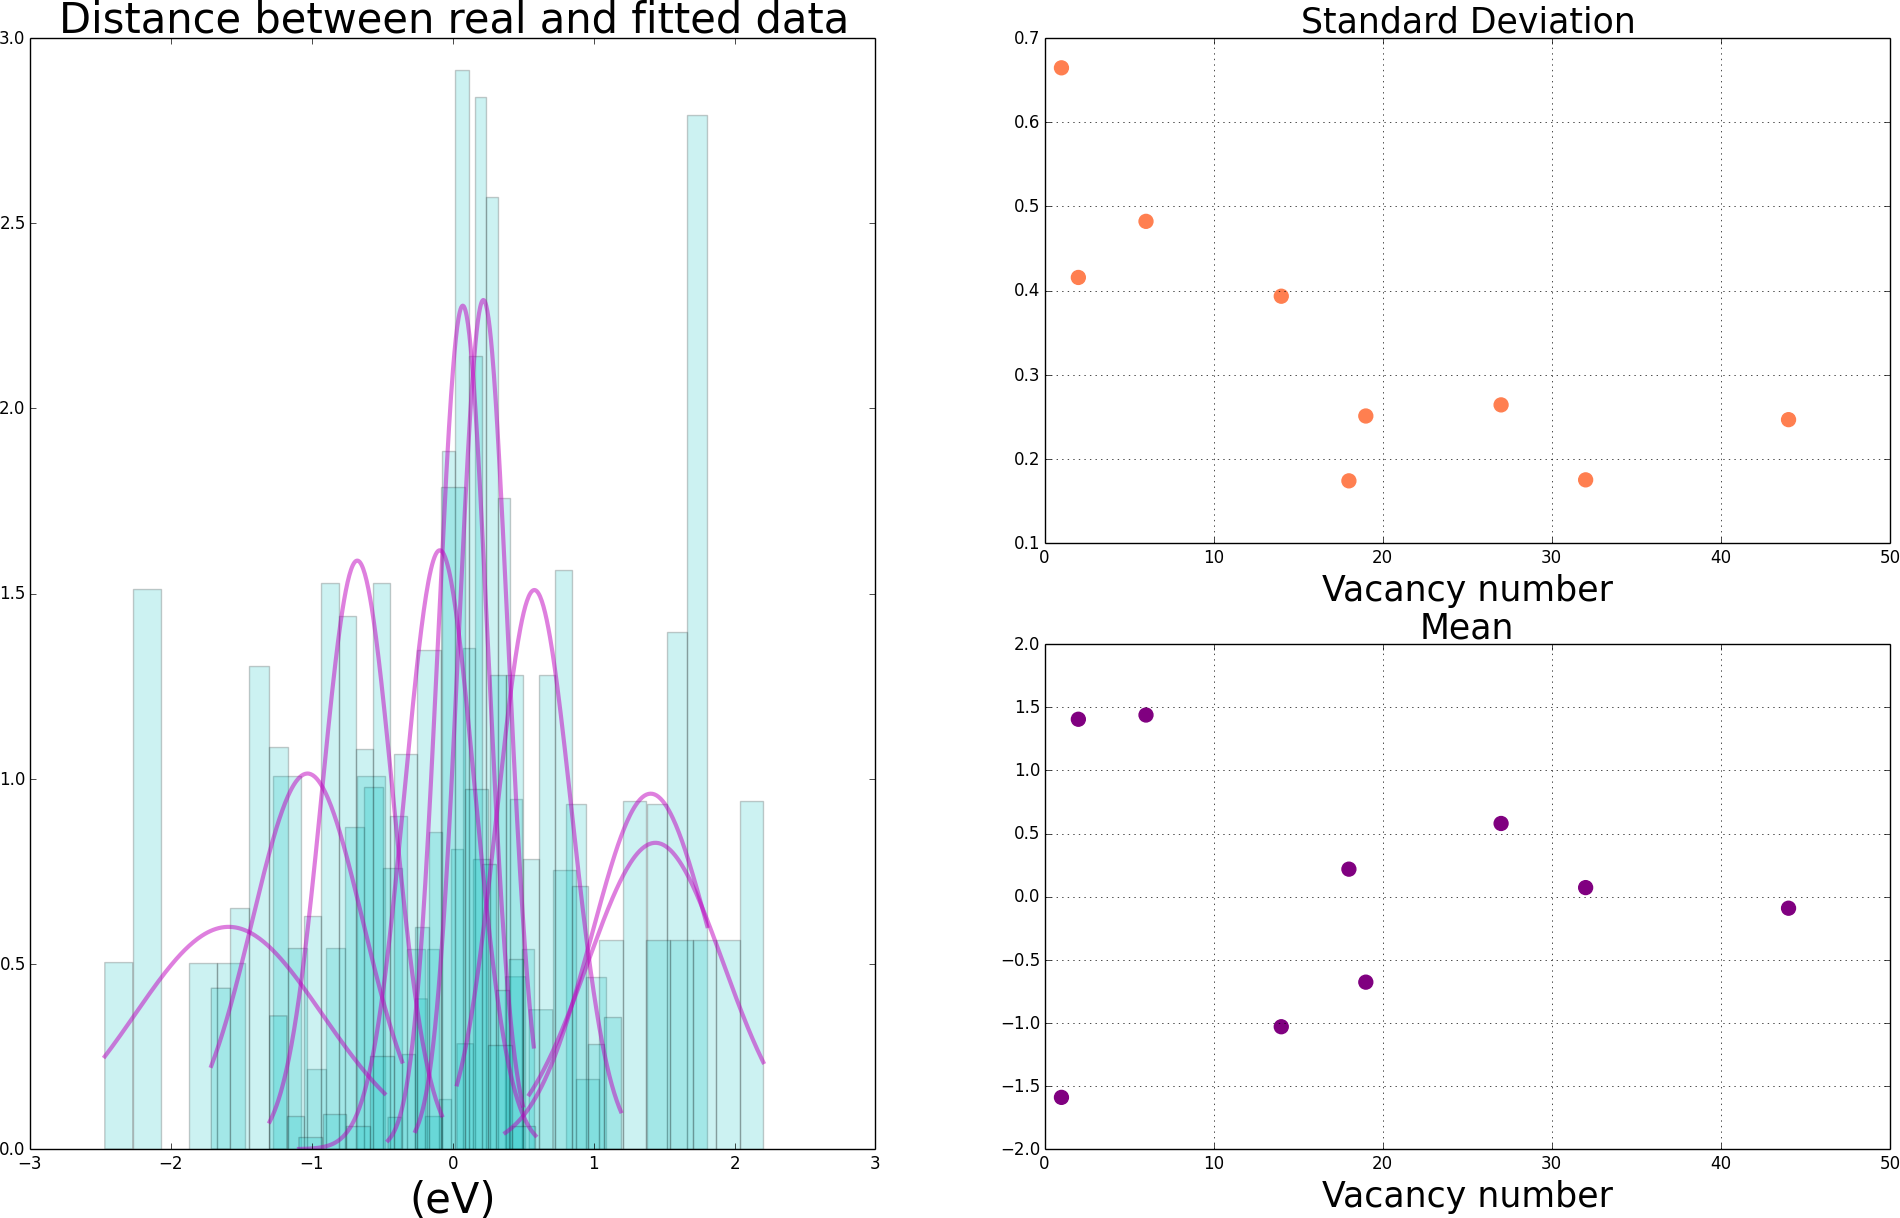
\includegraphics[width=0.8\textwidth]{CIFit1D_23331}
%     \end{figure}
% \end{frame}
% 
% \begin{frame}{Confidence Interval of the Fit}
% 	\begin{figure}
%         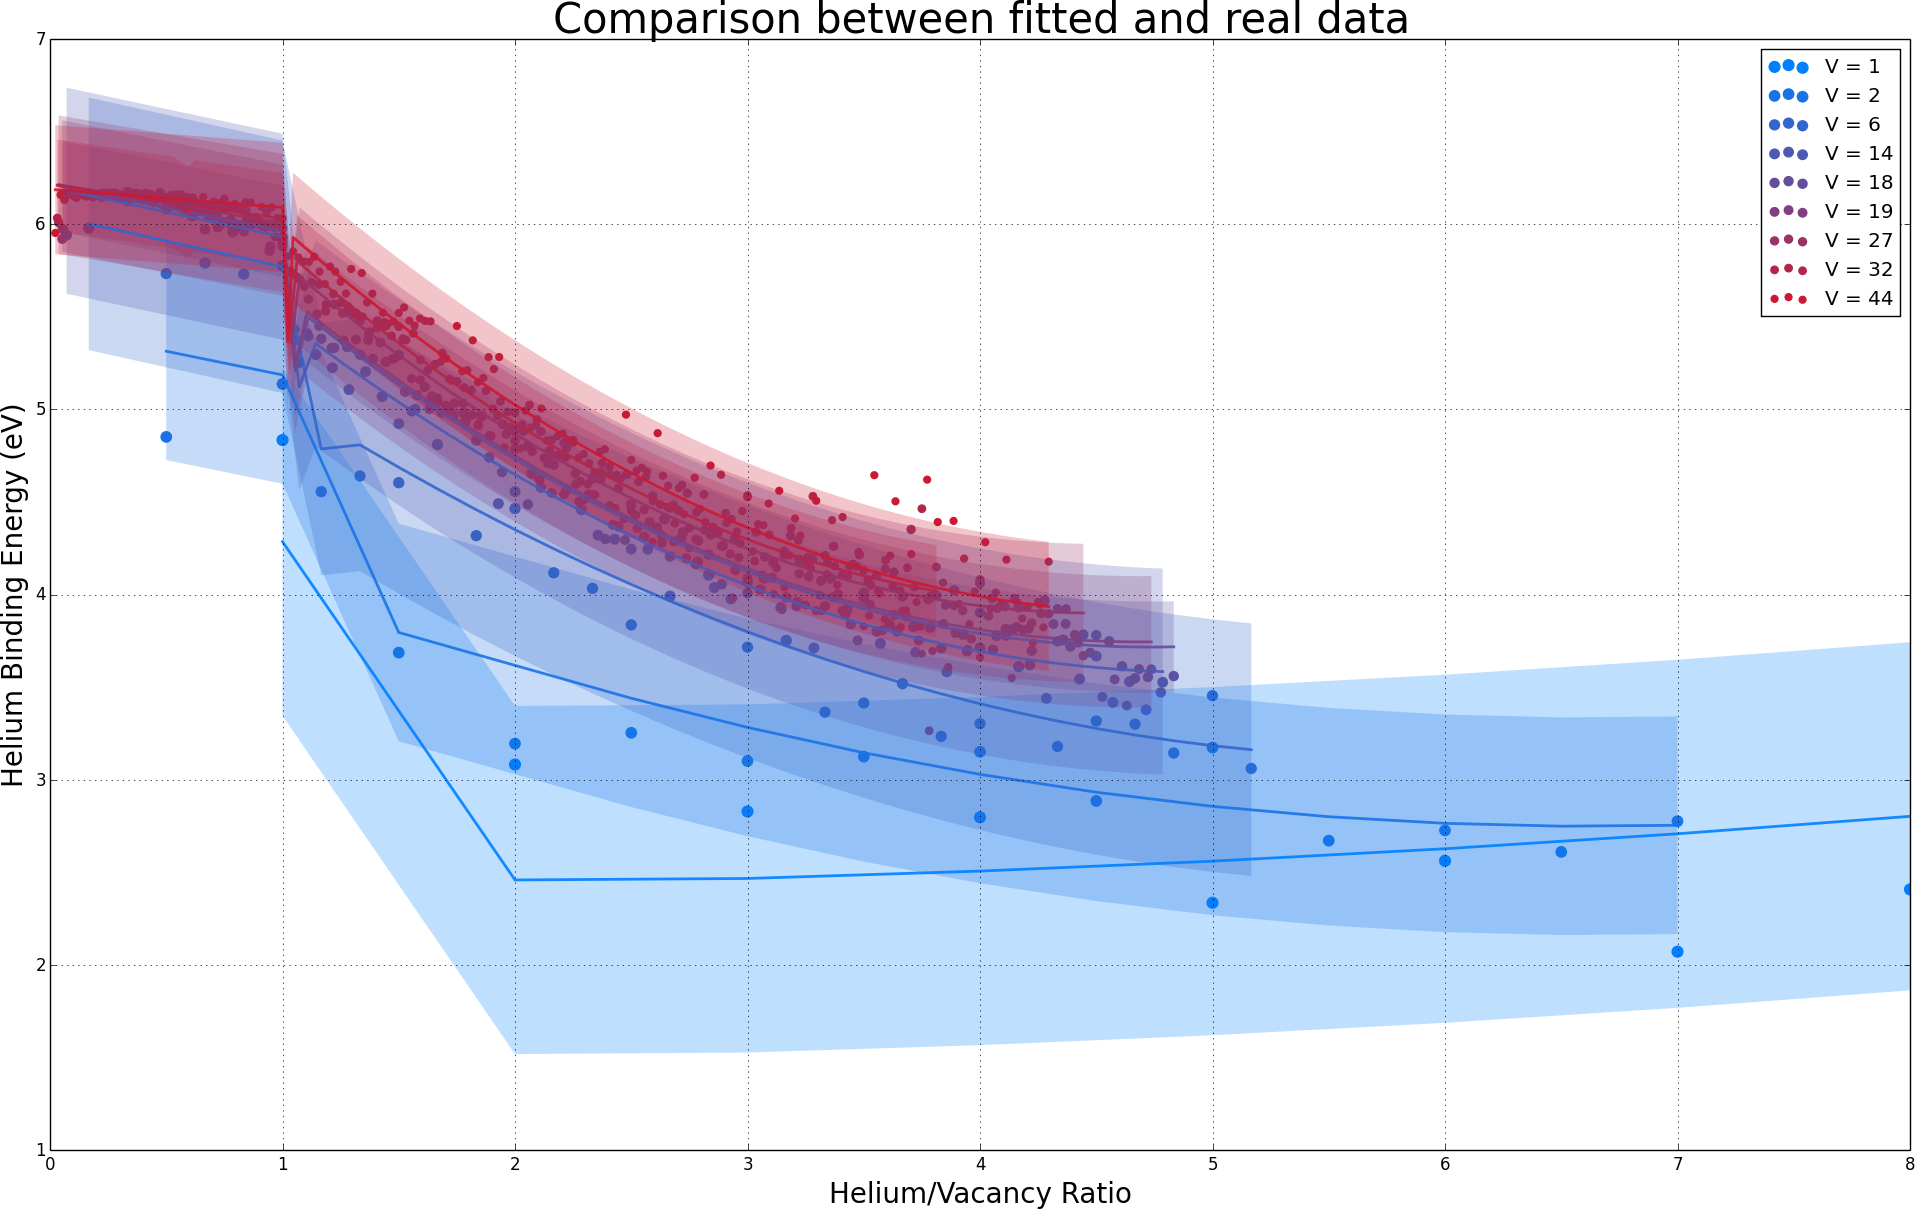
\includegraphics[width=0.9\textwidth]{CIComparison}
%     \end{figure}
% \end{frame}
% 
% \begin{frame}{Problem}
% 	\Large
% 	Most of the fit tried to give a non-decreasing function of He for V~$= 1$.
% \end{frame}
% 
% \begin{frame}{Fitting binding energies for V~$= 1,2$}
%      \vspace{3mm}
%      \large
%      Two options\ldots
%      \begin{itemize}
%            \item[$\blacktriangleright$] Due to the lack of data, use fit 
% 			described
%            in previous slides.
%            \item[$\blacktriangleright$] Acquire a good fit for V~$= 1,2$ 
% 			ONLY and
%            use previously described fit for all V~$> 2$ \newline
%      \end{itemize}
%      \normalsize
%      \vspace{-1.5mm}
%      \begin{figure}
%          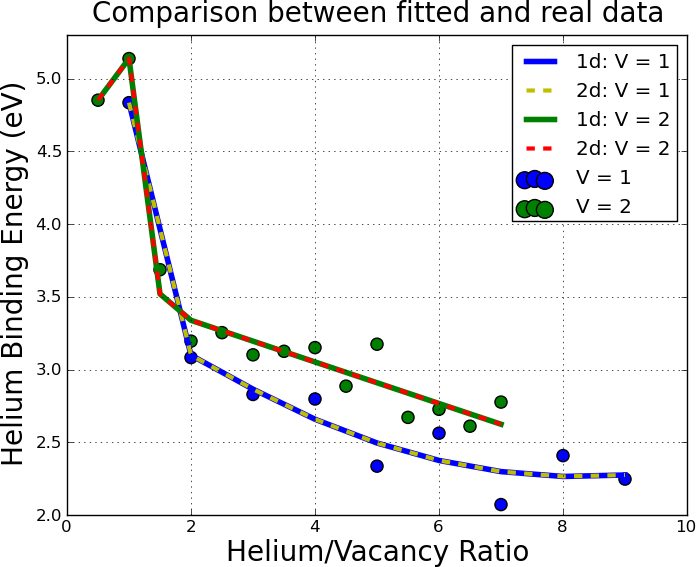
\includegraphics[width=0.6\linewidth]{V1_2_fit}
%      \end{figure}
% \end{frame}

\begin{frame}{Bayesian Inference Principle}
	\Large
	$$P(H|E) \propto P(E|H) \cdot P(H)$$ \newline

	\large
	\begin{itemize}
  		\item[$\blacktriangleright$] the \textbf{posterior} $P(H|E)$ (probability of
  		the hypothesis $H$ given the evidence $E$) that is infered
  		\item[$\blacktriangleright$] the \textbf{likelihood} $P(E|H)$ (probability
  		of the evidence $E$ given the hypothesis $H$)
  		\item[$\blacktriangleright$] and the \textbf{prior} $P(H)$ that gathers all
  		the information one had before the evidence $E$ was observed
	\end{itemize}
	
\end{frame}

\begin{frame}{Bayesian Inference in UQTk}
	\large
	Markov Chain Monte Carlo (MCMC) Method: Metropolis-Hastings algorithm with
	adaptive proposal distribution. \newline
    \begin{itemize}
    	\item[$\blacktriangleright$] Metropolis-Hastings: the step $Y$ at $t$ is
    	kept with a probability $\alpha$
    	
    	$$\alpha = \text{min}(1, \frac{\pi (Y)}{\pi (X_{t-1})})$$
    	with $\pi$ the target distribution. \newline
    	
    	\item[$\blacktriangleright$] Adaptive part: the proposal distribution (to go from a step
    to the next one) is a function of all the previous step.
    \end{itemize}
\end{frame}

\begin{frame}{Bayesian Inference in UQTk: Example}
	\large
    \begin{itemize}
    	\item[$\blacktriangleright$] Generate points from $-20$ to $20$ following
    	$$f(x) = -1 + 0.4 x - 0.12 x^2 + 0.032 x^3$$
    	
    	with a gaussian noise of amplitude $5$. \newline
    	
    	\item[$\blacktriangleright$] Model them with
    	$$M(x) = \texttt{param\_a} + \texttt{param\_b} \cdot x + \texttt{param\_c}
    	\cdot x^2 + \texttt{param\_d} \cdot x^3$$
    	
    	and the same gaussian noise.
    \end{itemize}
\end{frame}

\begin{frame}{Bayesian Inference in UQTk: Example}
     \begin{figure}
         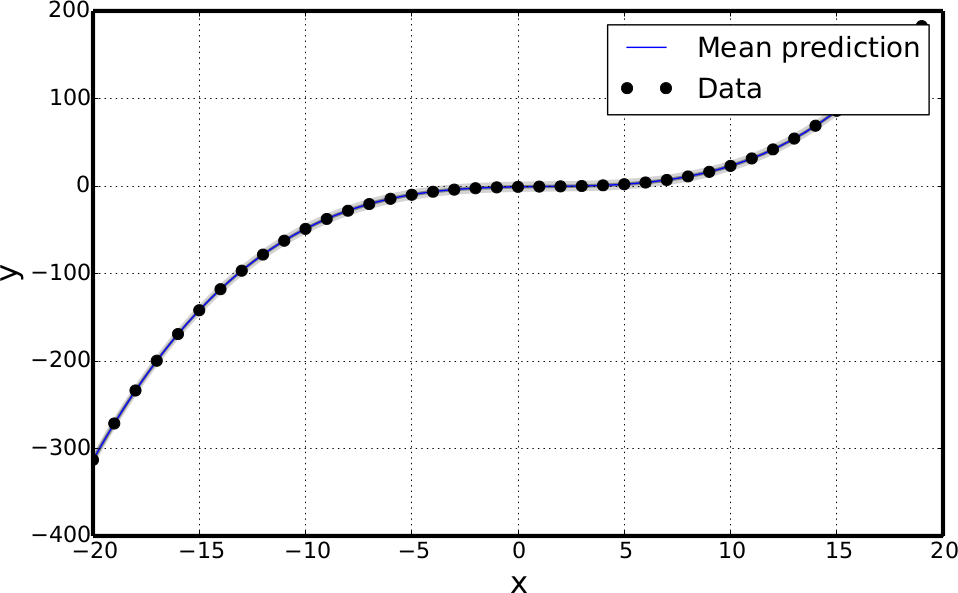
\includegraphics[width=0.45\textwidth]{result}
         \hspace{0.5in}
         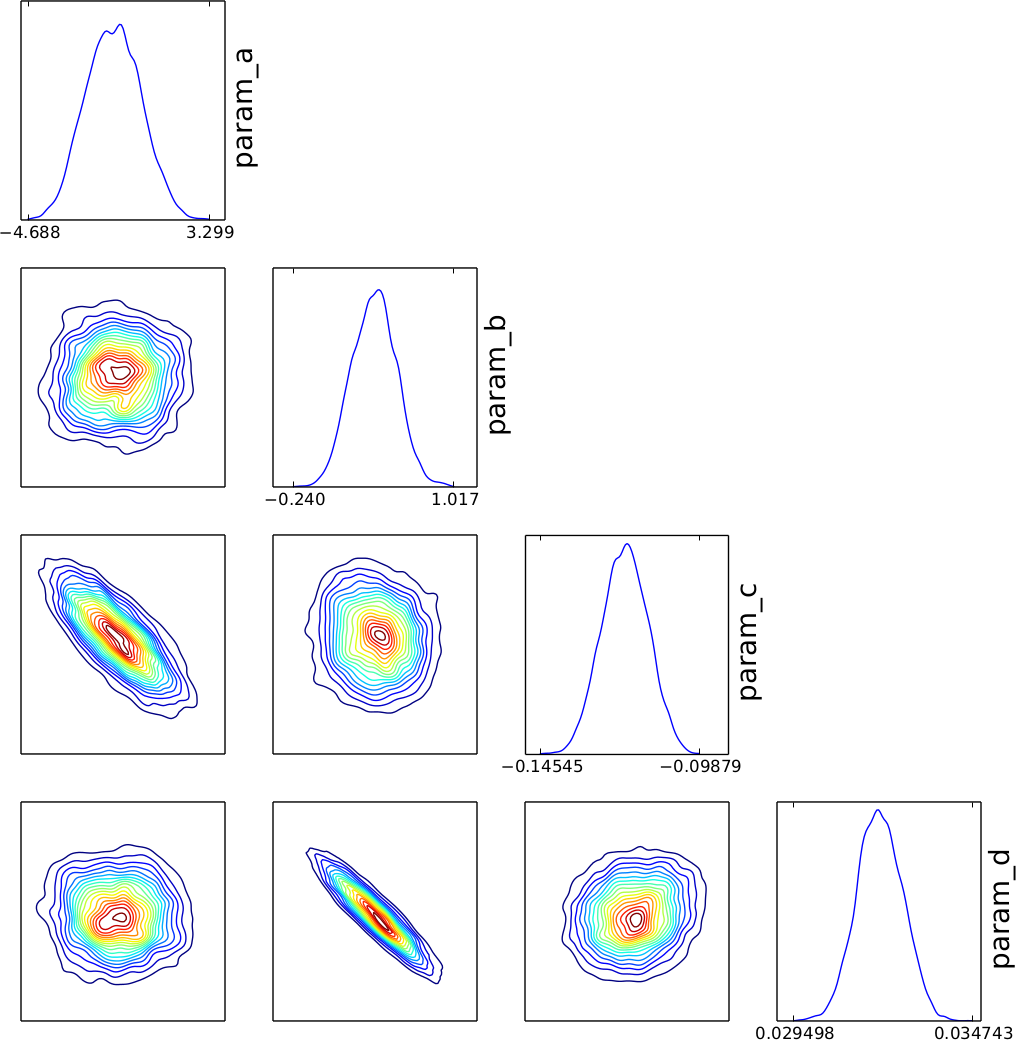
\includegraphics[width=0.3\textwidth]{posteriorSummary}
         \hspace{0.4in}
     \end{figure}
     \begin{figure}
         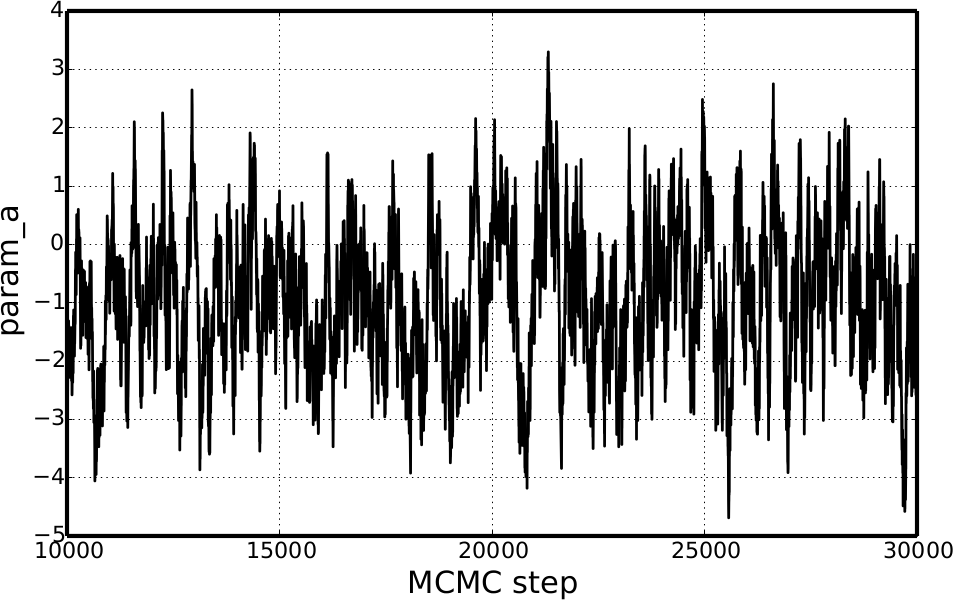
\includegraphics[width=0.45\textwidth]{chainExample}
         \hspace{0.1in}
         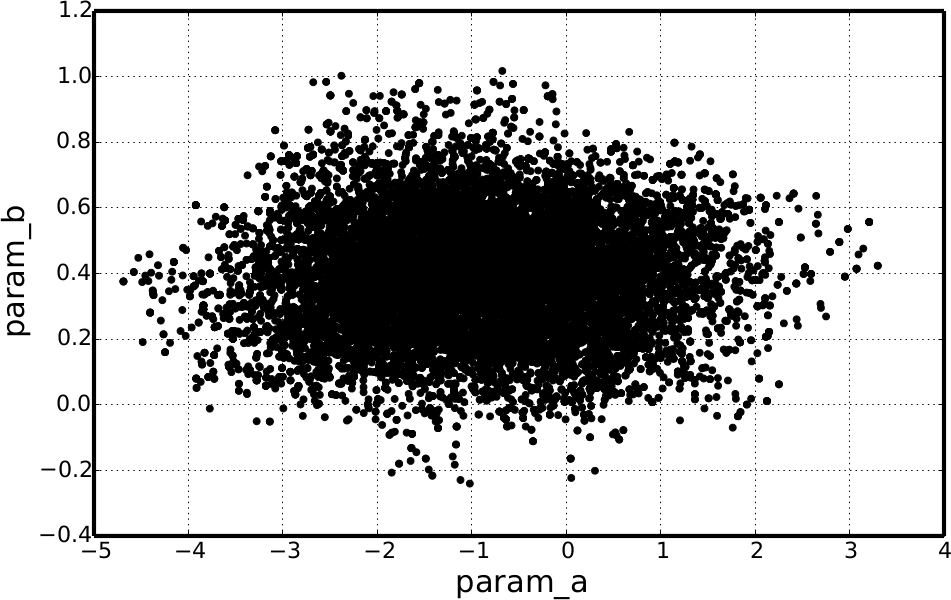
\includegraphics[width=0.45\textwidth]{chain2DExample}
     \end{figure}
\end{frame}

\begin{frame}{Bayesian Inference in UQTk: $V = 27$ Formation Energies}
	\large
	    \begin{itemize}
    	\item[$\blacktriangleright$] Suppose the following function is used to fit
    	the data
    	$$f(x) = a + b x + c x^2 + d x^3 + f x^4 + g x^5$$
    	\item[$\blacktriangleright$] Fitting the data using GNUplot gives
    	\begin{align*}
    	a = 49.0722,~&b = -1.0619, c = -4.87474, d = 9.92562, \\
    	&f = -2.47767, g = 0.200702
    	\end{align*}
    	\item[$\blacktriangleright$] Model the data with
    	\begin{align*}
    	M(x) = \texttt{param\_a} &+ \texttt{param\_b} \cdot x - \texttt{param\_c}
    	\cdot x^2 + \texttt{param\_d} \cdot x^3 \\
    	 & \texttt{param\_f} \cdot x^4 + \texttt{param\_g} \cdot x^5
    	\end{align*}
    	to infer $6$~parameters.
    \end{itemize}
\end{frame}

\begin{frame}{Bayesian Inference in UQTk: $V = 27$ Formation Energies}
     \begin{figure}
         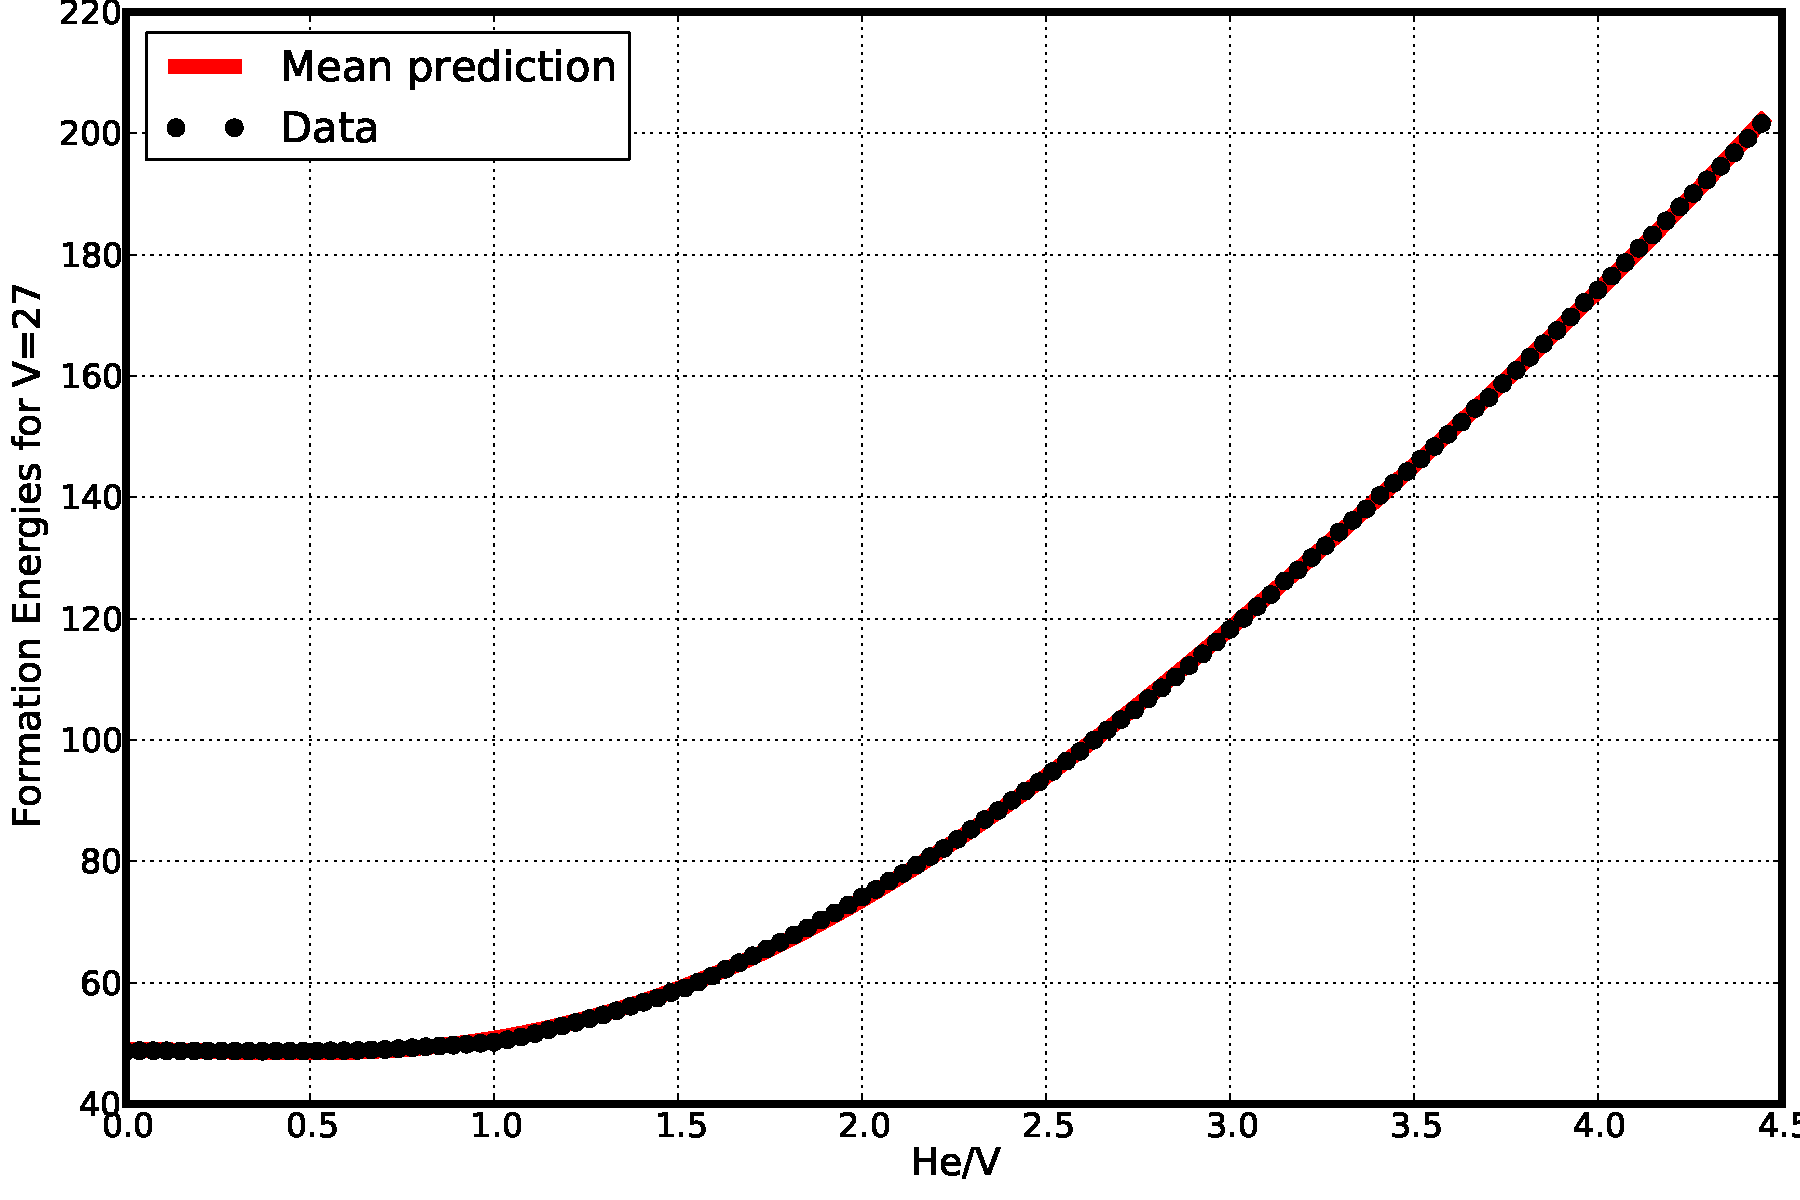
\includegraphics[width=0.5\textwidth]{prob5_postpred}
     \end{figure}
     
     \begin{figure}
         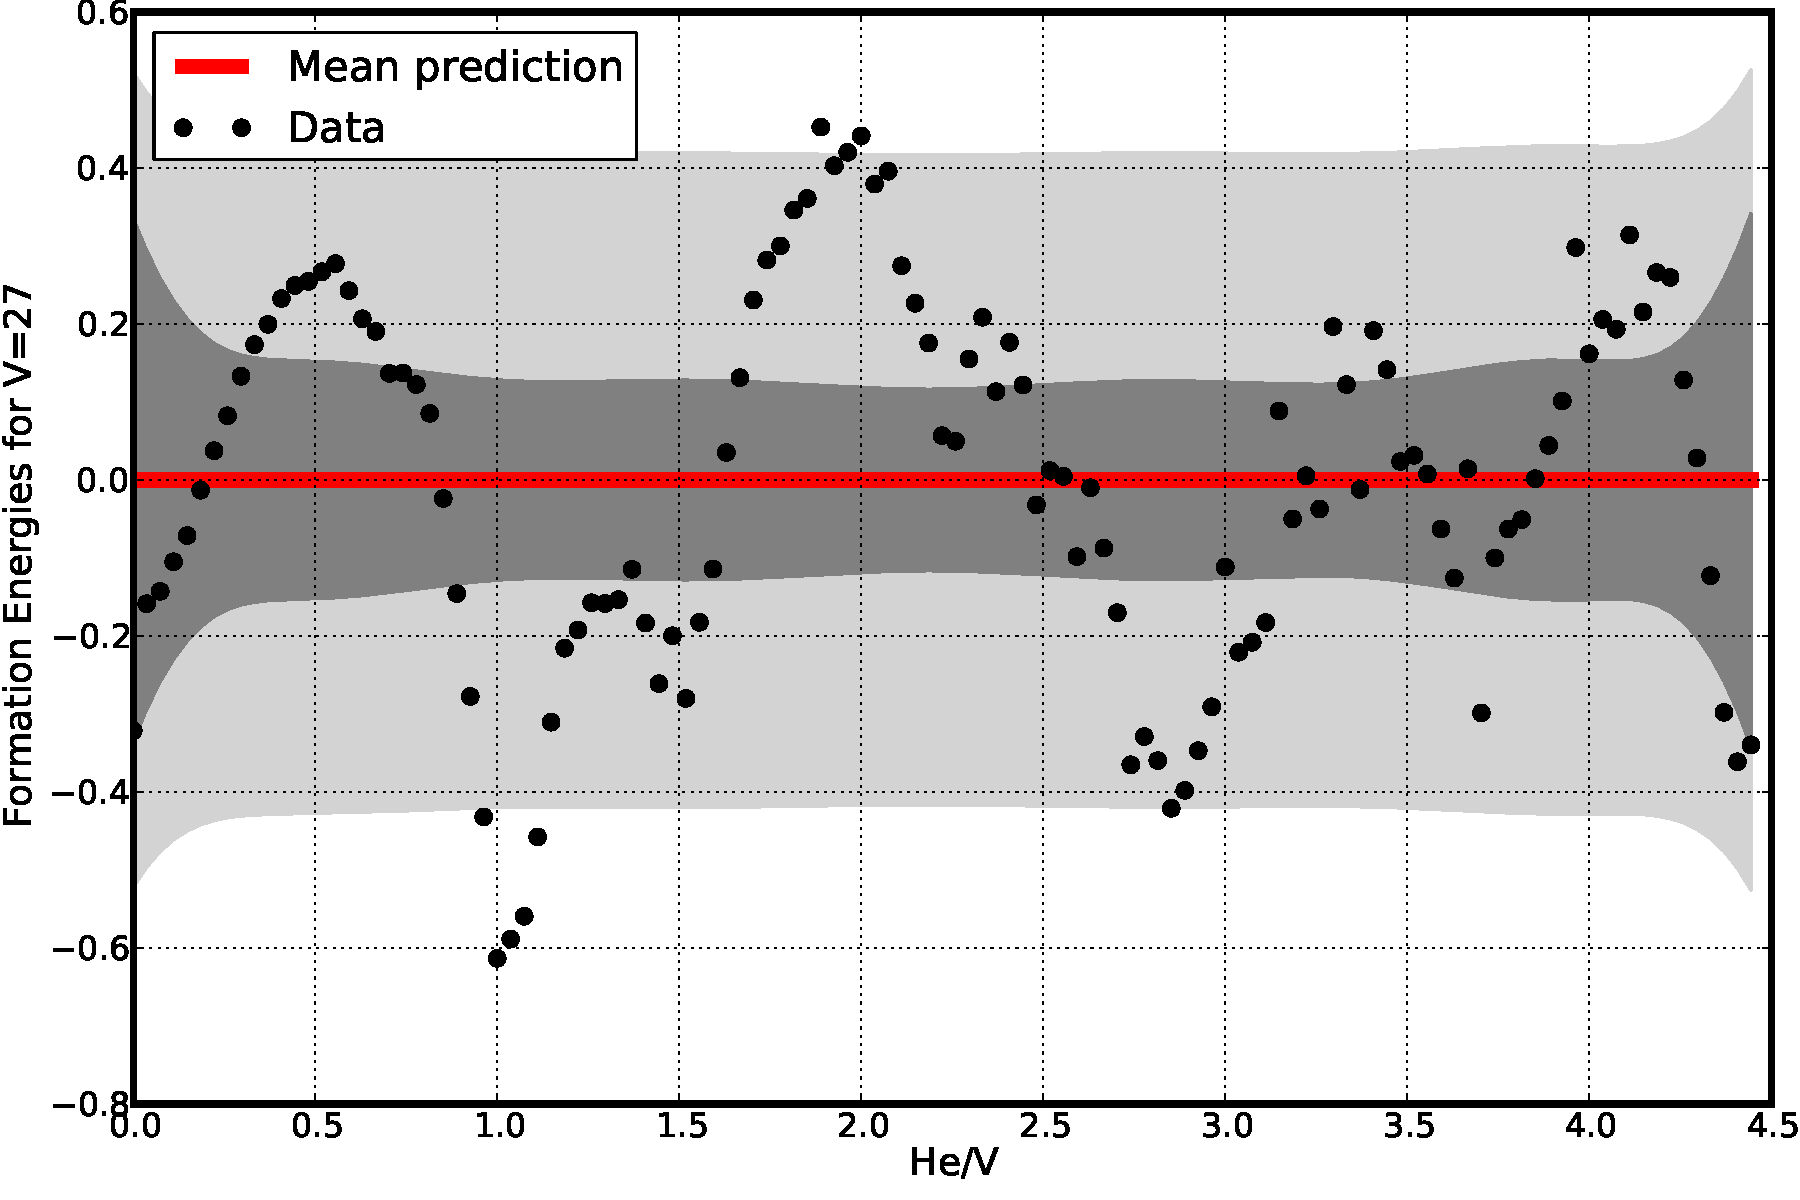
\includegraphics[width=0.5\textwidth]{prob5_postpred_noise}
     \end{figure}
\end{frame}

\begin{frame}{Bayesian Inference in UQTk: $V = 27$ Formation Energies}
  	\begin{columns}[onlytextwith]
    	\begin{column}{0.5\textwidth}
      		\begin{figure}
        		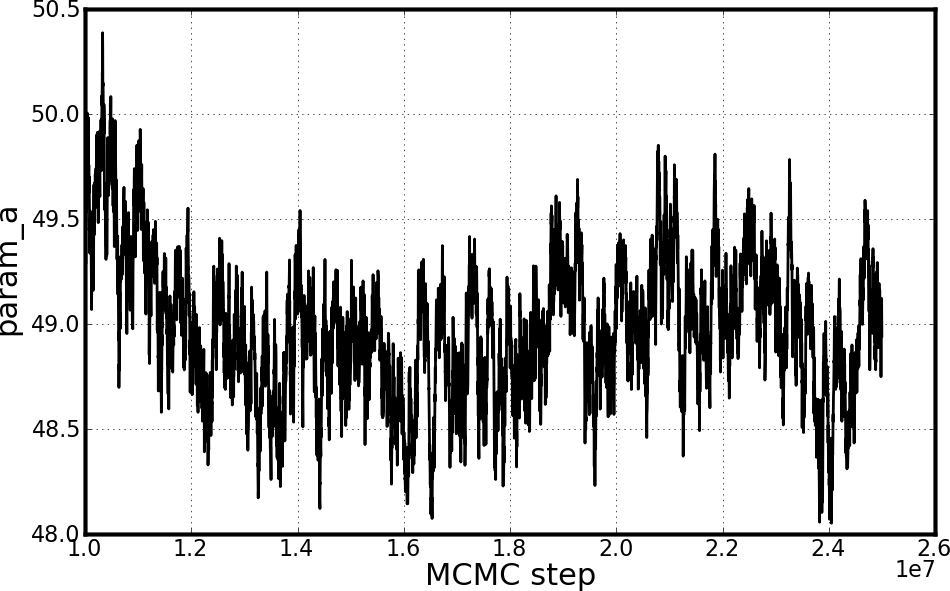
\includegraphics[width=0.95\textwidth]{prob5_chn_param_a}
      		\end{figure}
      		\begin{figure}
        		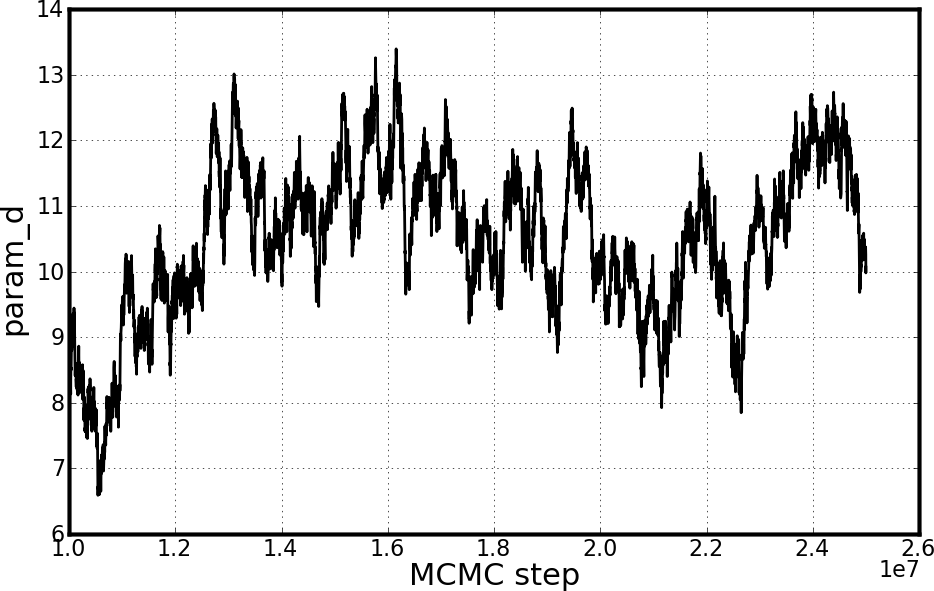
\includegraphics[width=0.95\textwidth]{prob5_chn_param_d}
      		\end{figure}
    	\end{column}  
    	\begin{column}{0.5\textwidth}
      		\begin{figure}
        		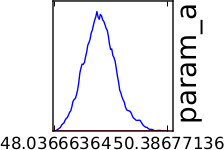
\includegraphics[height=0.2\textheight]{posterior_a}
        		\hspace{0.1in}
        		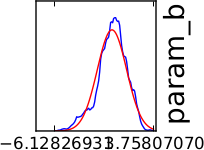
\includegraphics[height=0.2\textheight]{posterior_b}
      		\end{figure}
      		
      		\begin{figure}
        		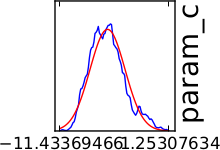
\includegraphics[height=0.2\textheight]{posterior_c}
        		\hspace{0.1in}
        		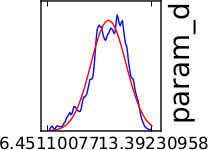
\includegraphics[height=0.2\textheight]{posterior_d}
      		\end{figure}
      		
      		\begin{figure}
        		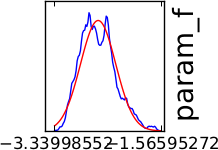
\includegraphics[height=0.2\textheight]{posterior_f}
        		\hspace{0.1in}
        		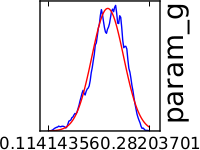
\includegraphics[height=0.2\textheight]{posterior_g}
      		\end{figure}
    	\end{column}
  	\end{columns}
\end{frame}

\begin{frame}{Next Steps}
	\Large
    \begin{itemize}
    	\item[$\blacktriangleright$] See how the parameters scale from one V number
    	to the next in order to determine a function that will fit the data.
    	\newline
    	
    	\item[$\blacktriangleright$] Conduct a preliminary global sensitivity
    	analysis on Xolotl using this function as an input.
    \end{itemize}
\end{frame}

\begin{frame}{Scaling of the Parameters with Python Fit}
	\begin{figure}
        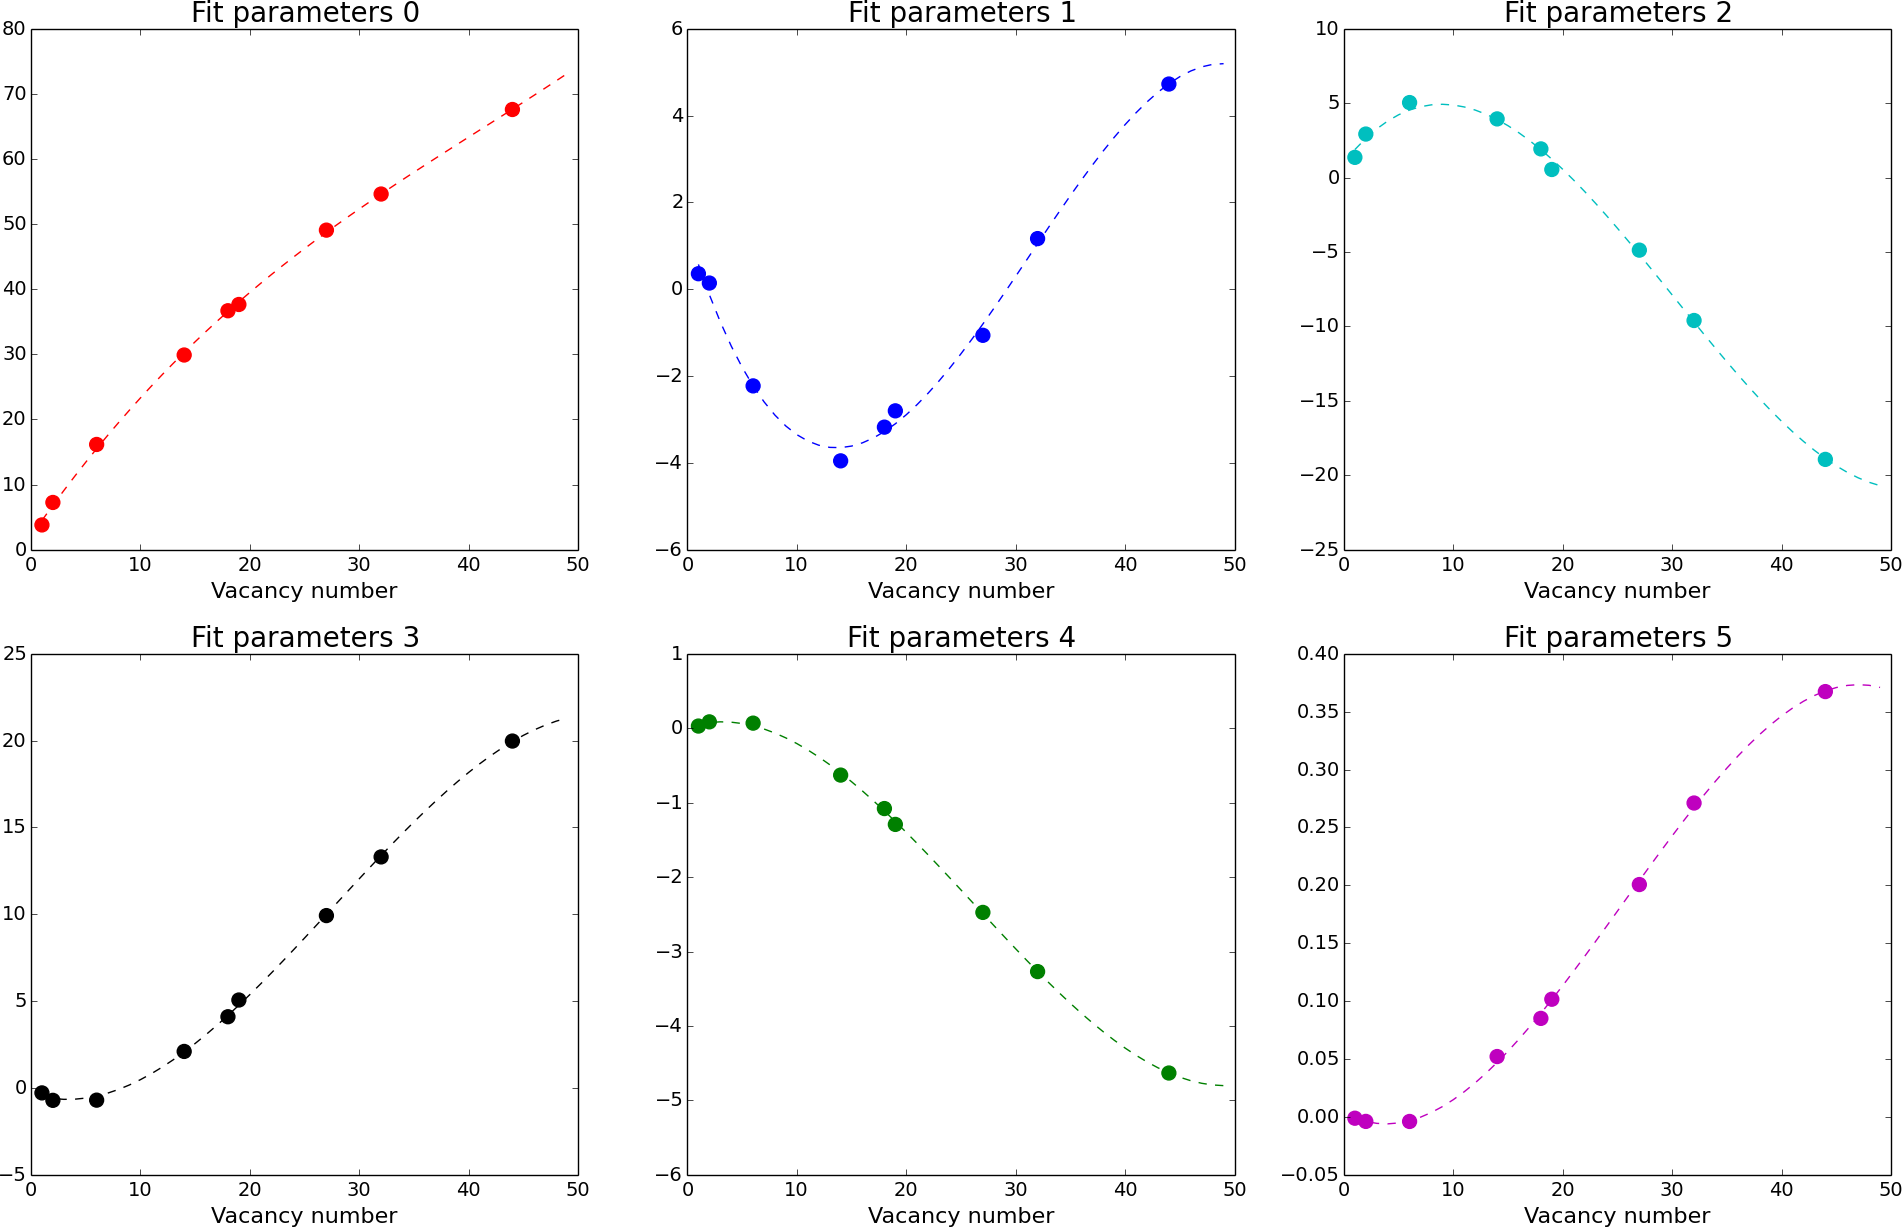
\includegraphics[width=0.95\textwidth]{parametersIN}
    \end{figure}
\end{frame}

\begin{frame}{Scaling of the Parameters with Python Fit}
	\begin{figure}
        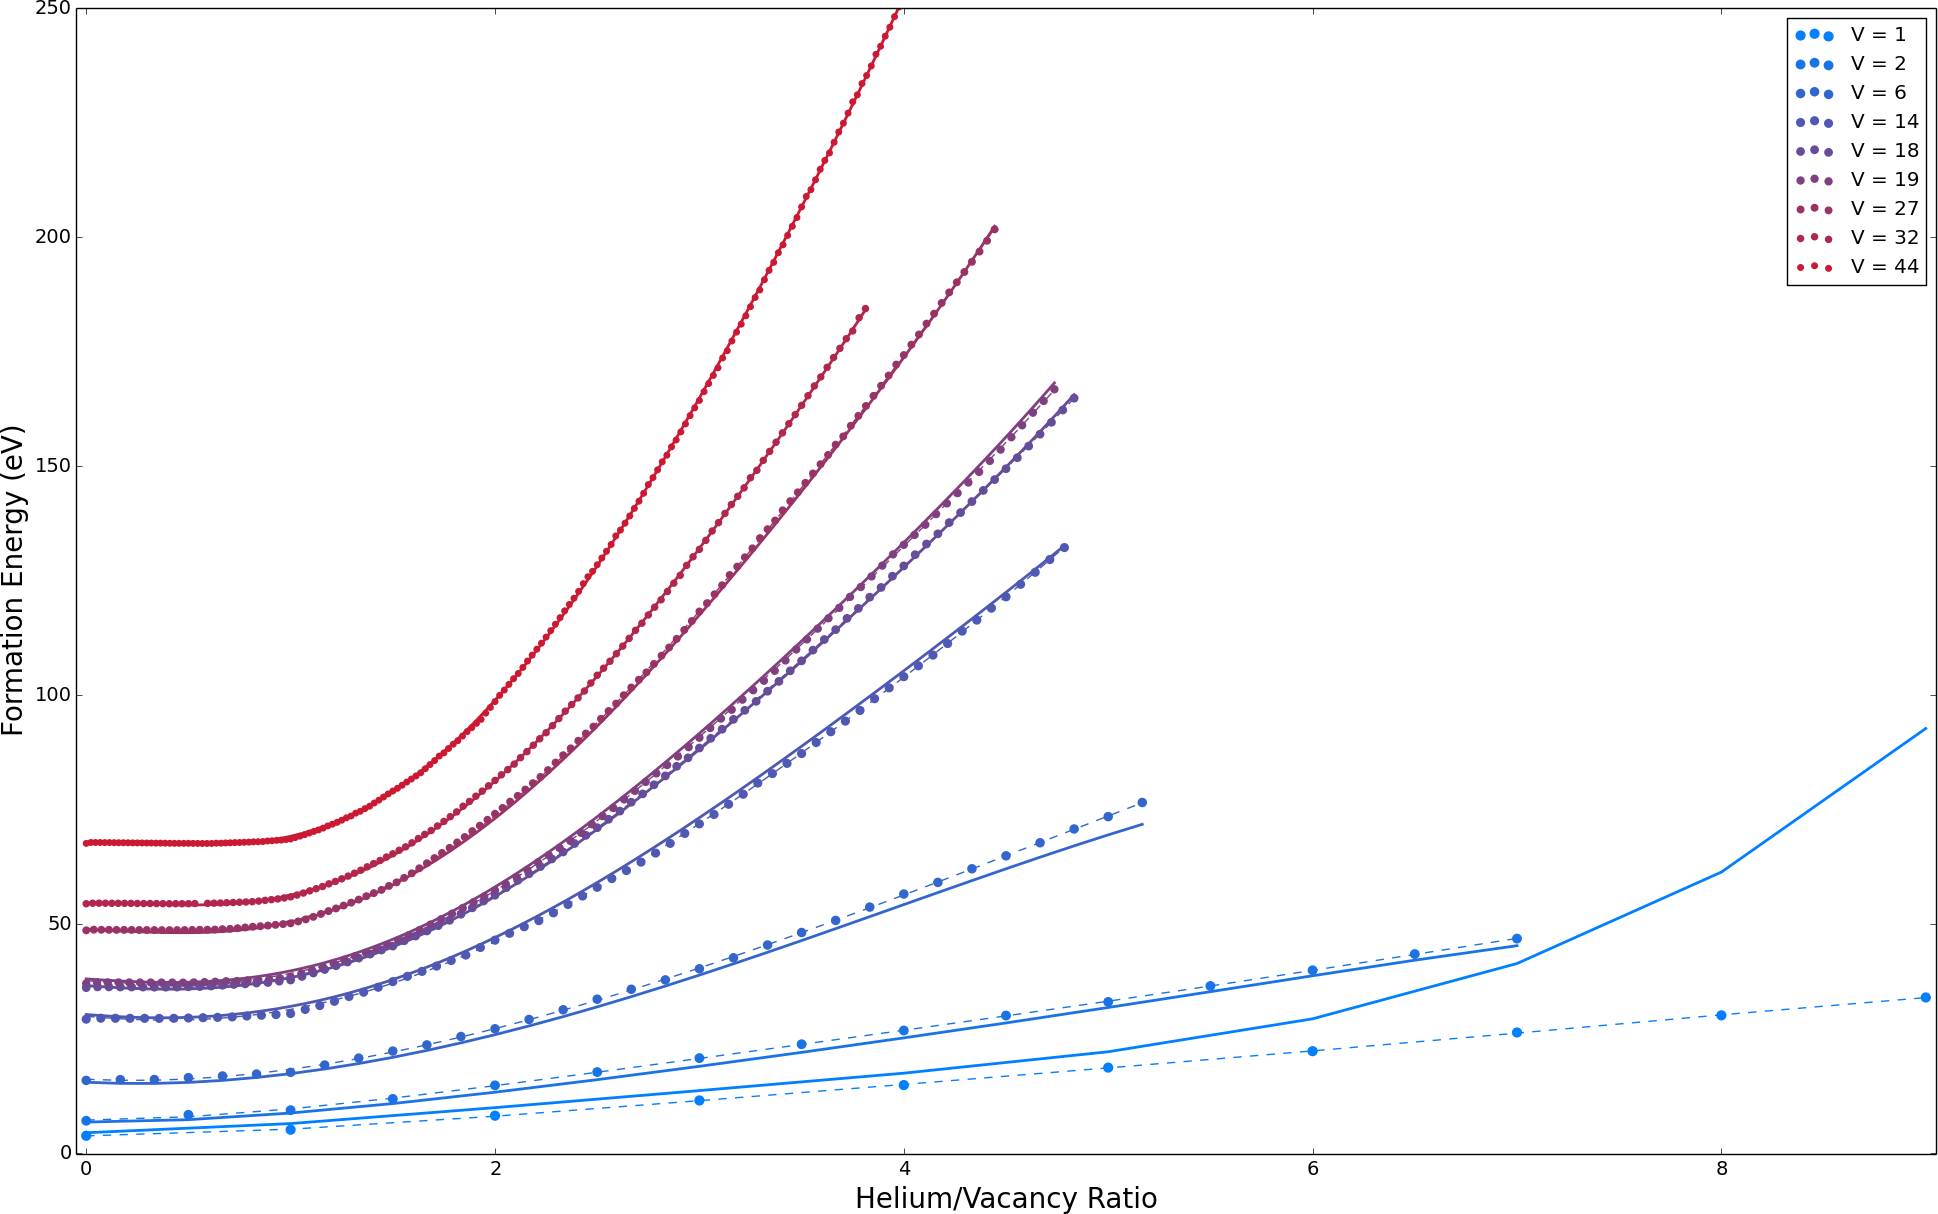
\includegraphics[width=0.95\textwidth]{energyIN}
    \end{figure}
\end{frame}

\begin{frame}{Scaling of the Parameters with Python Fit}
	\begin{figure}
        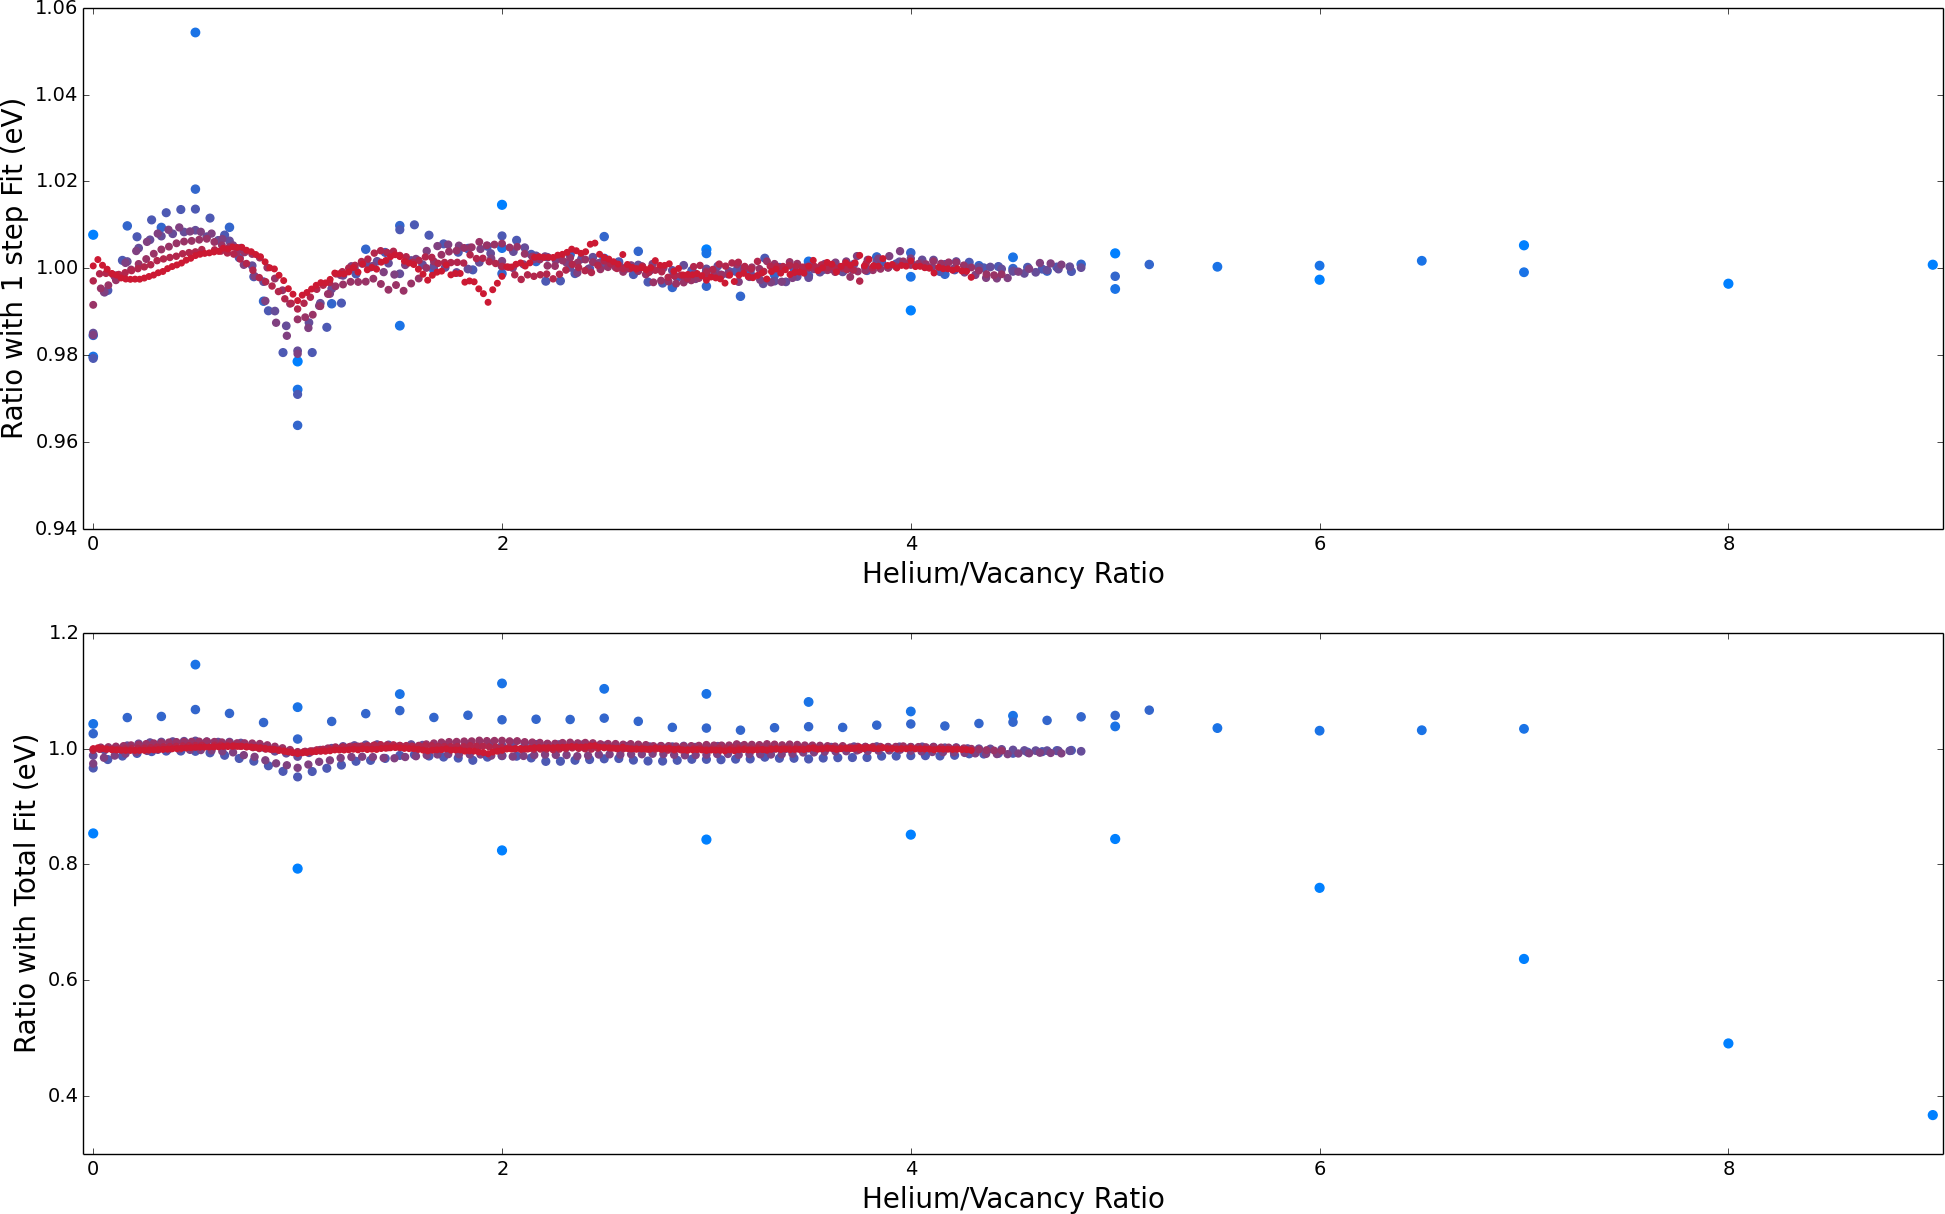
\includegraphics[width=0.95\textwidth]{ratioIN}
    \end{figure}
\end{frame}

\begin{frame}{Excluding V~$=1, 2$}
	\begin{figure}
        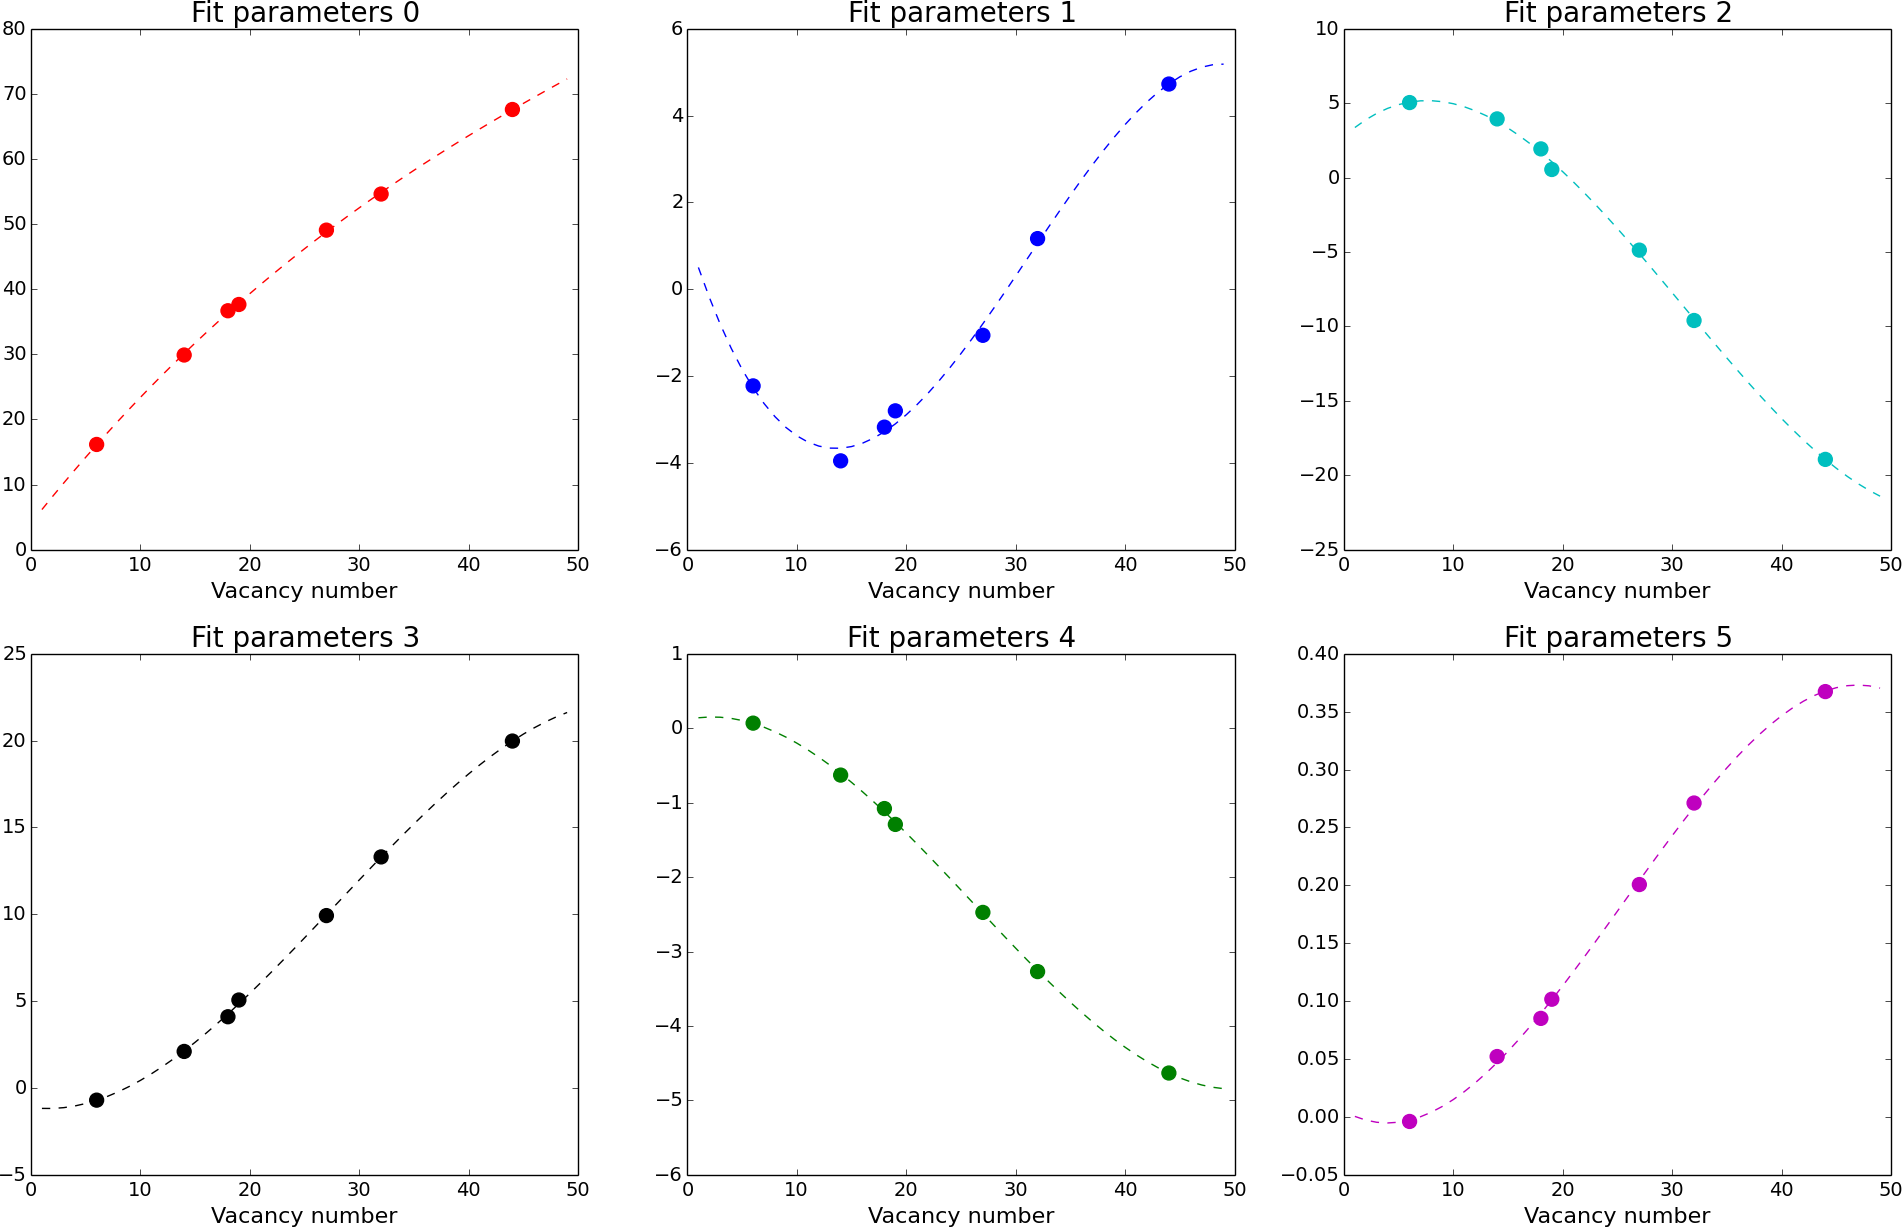
\includegraphics[width=0.95\textwidth]{parametersEX}
    \end{figure}
\end{frame}

\begin{frame}{Excluding V~$=1, 2$}
	\begin{figure}
        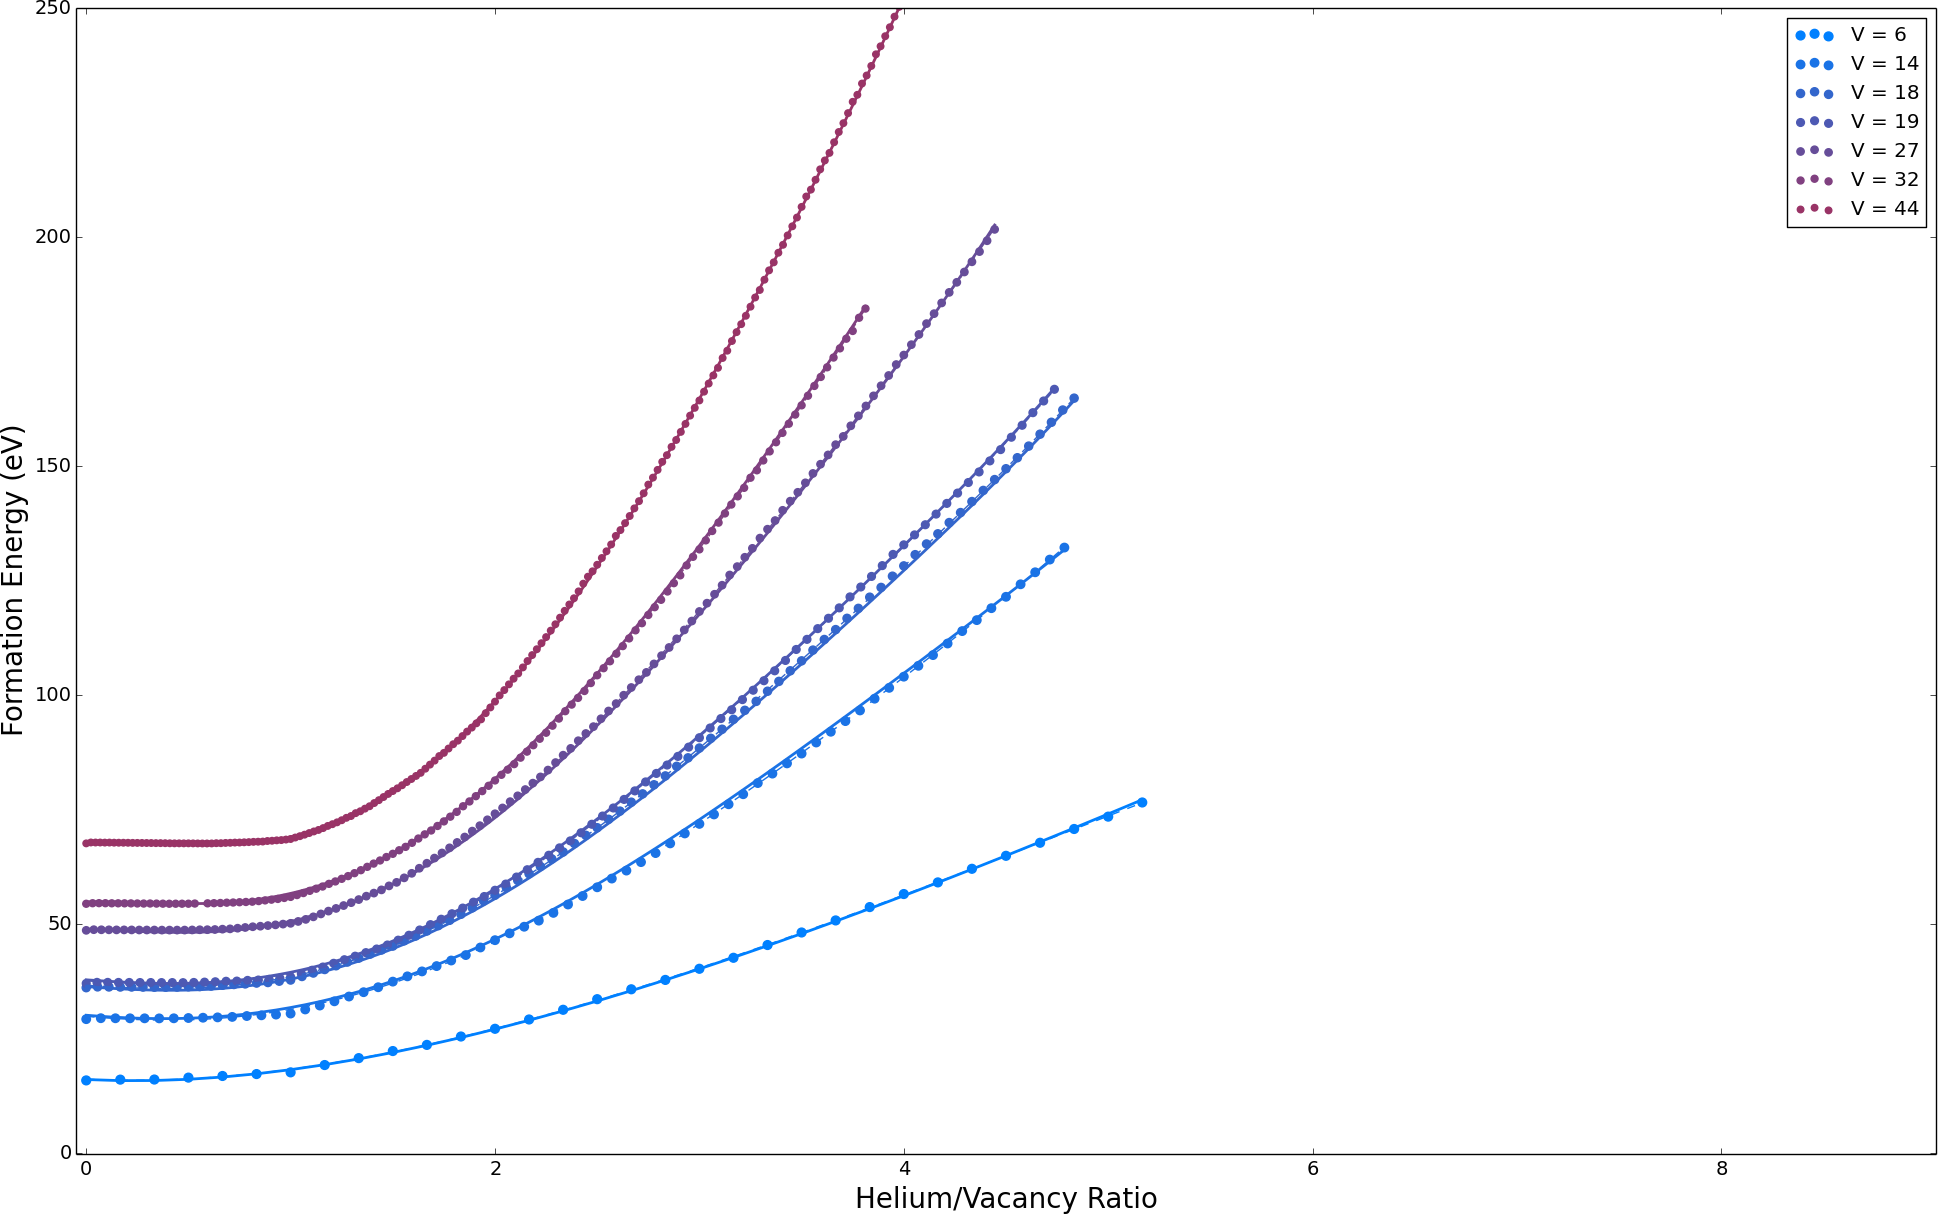
\includegraphics[width=0.95\textwidth]{energyEX}
    \end{figure}
\end{frame}

\begin{frame}{Excluding V~$=1, 2$}
	\begin{figure}
        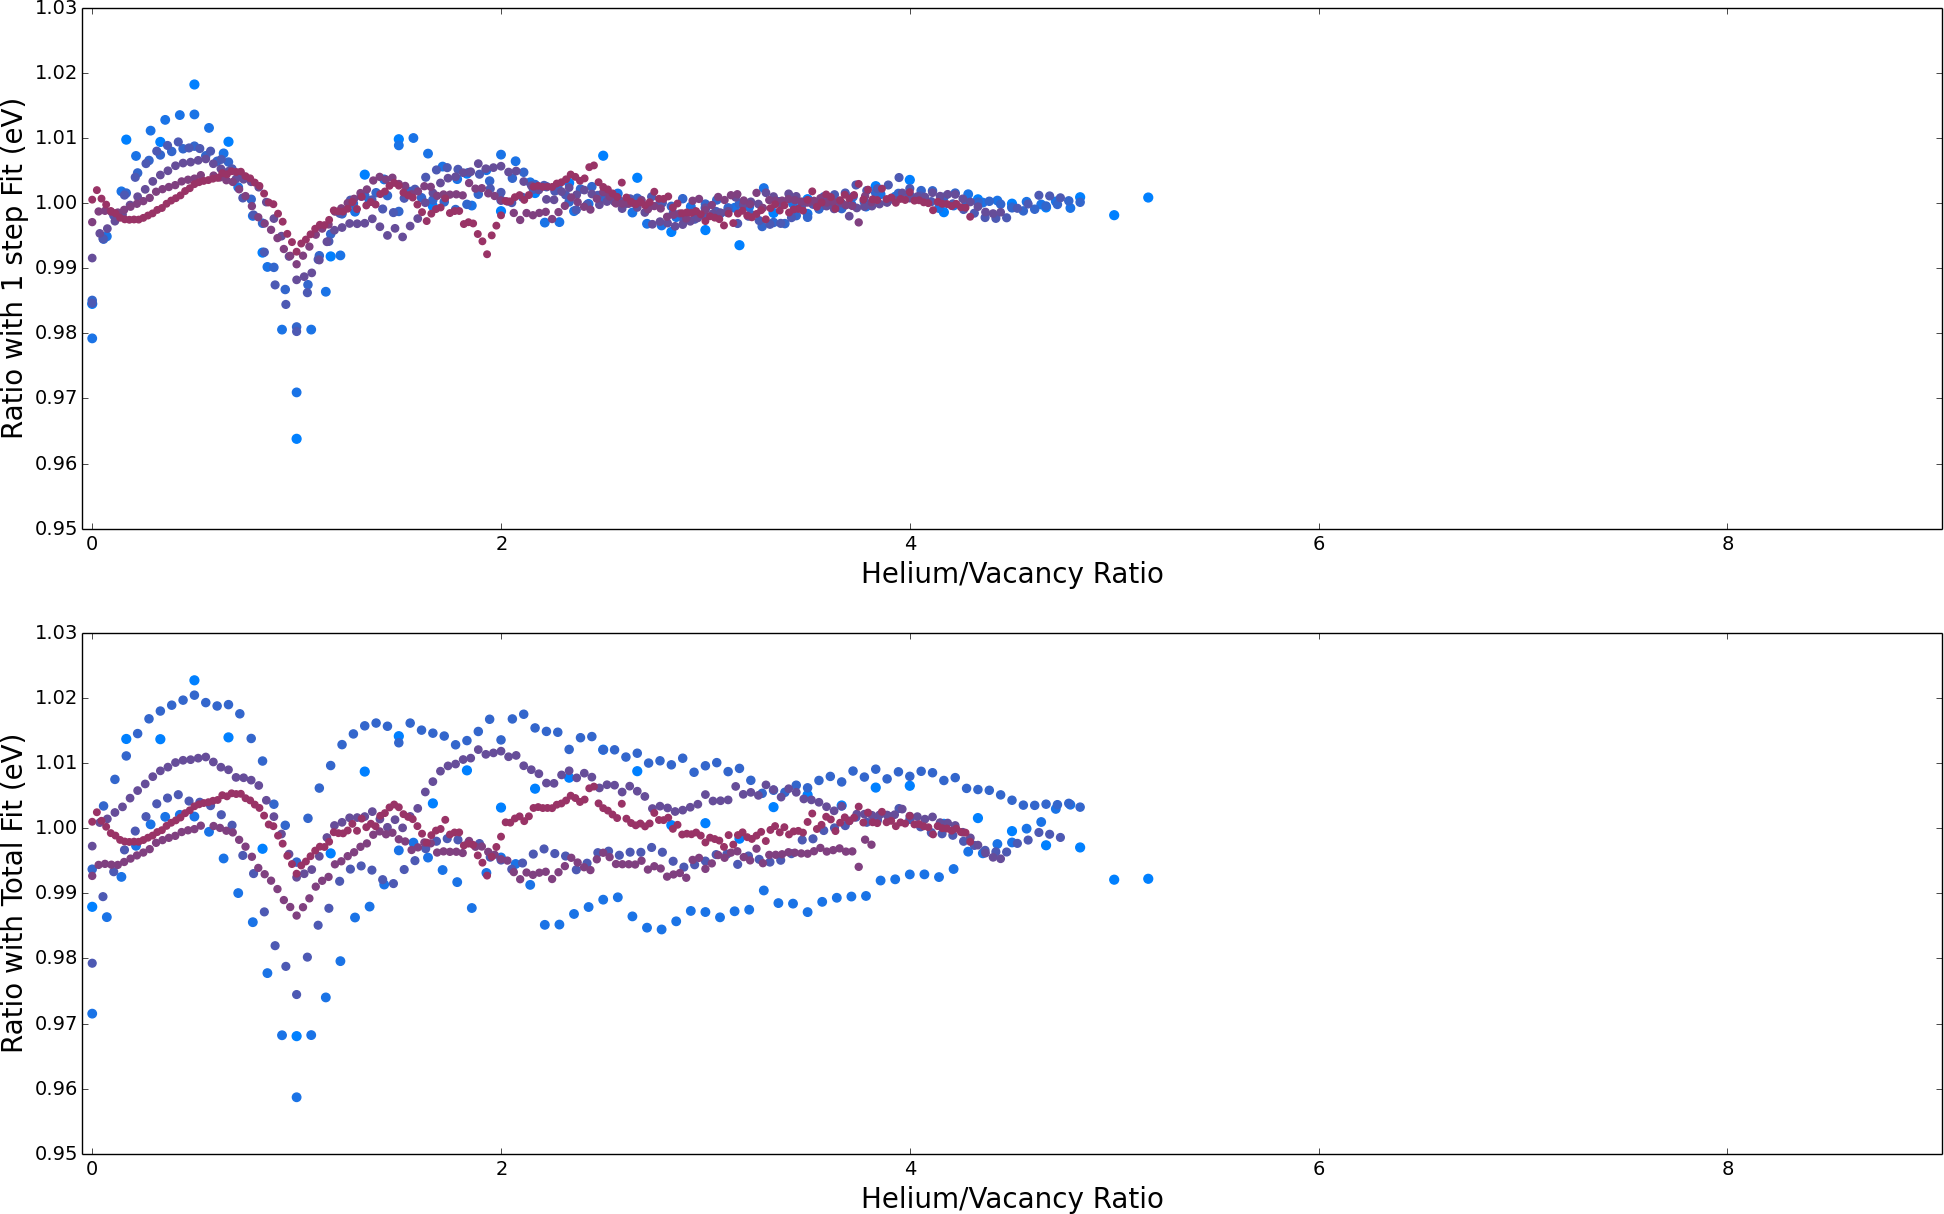
\includegraphics[width=0.95\textwidth]{ratioEX}
    \end{figure}
\end{frame}

% \begin{frame}{Bayesian Inference in UQTk: Burn-in}
% 	\large
% 	Steps needed for the chain to converge, must not be used to obtain the target
% 	distribution.
%      \begin{figure}
%          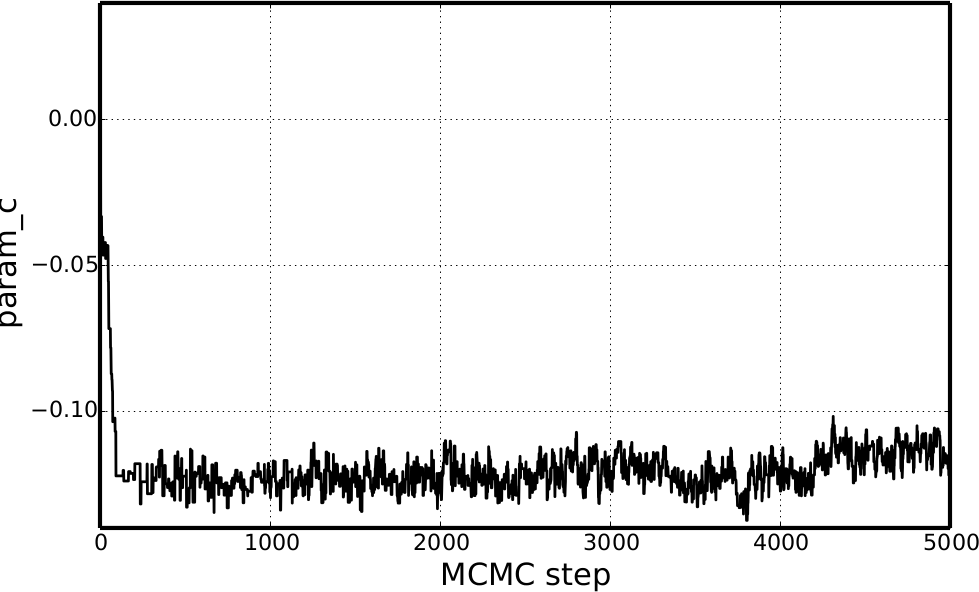
\includegraphics[width=0.7\textwidth]{burninExample}
%      \end{figure}
% \end{frame}
% 
% \begin{frame}{Bayesian Inference in UQTk: $\gamma$ parameter}
% 	\large
% 	``Size of the step", needs to be fine tuned:
%     \begin{itemize}
%     	\item[$\blacktriangleright$] if too small (high acceptance rate)
%      	\begin{figure}
%          	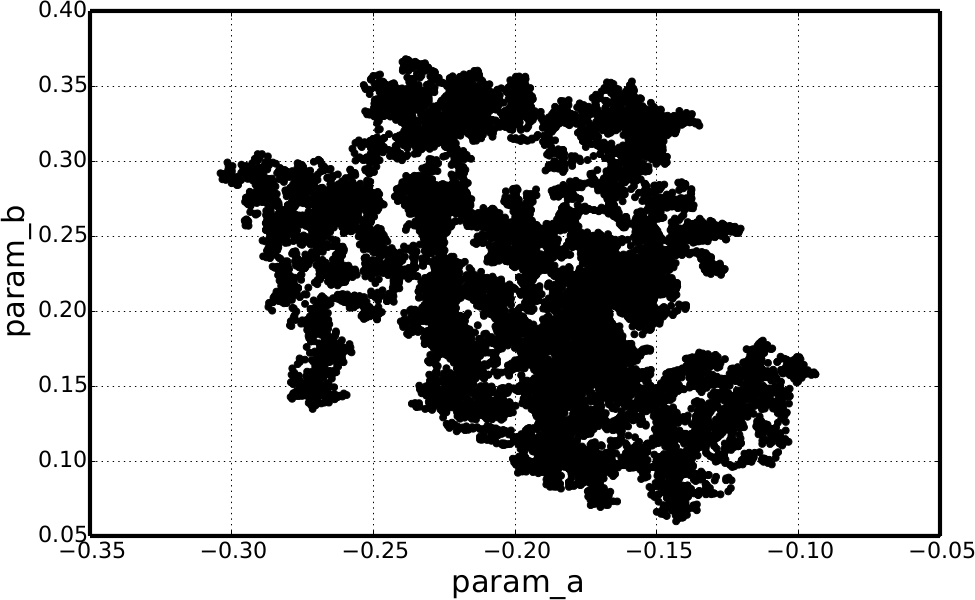
\includegraphics[width=0.6\textwidth]{smallGammaExample}
%      	\end{figure}
%     	
%     	\item[$\blacktriangleright$] if too big: low acceptance rate.
%     \end{itemize}
% \end{frame}

% \begin{frame}{Bayesian Inference in UQTk: $V = 27$ Formation Energies}
% 	\large
% 	    \begin{itemize}
%     	\item[$\blacktriangleright$] Suppose the following function is used to fit
%     	the data 
%     	$$f(x) = a + b x + c x^2 + d x^3 + g x^4 + h x^5$$
%     	\item[$\blacktriangleright$] Fitting the data using GNUplot gives
%     	\begin{align*}
%     	a = 49.0722, &b = -1.0619, c = -4.87474, d = 9.92562, \\
%     	&g = -2.47767, h = 0.200702
%     	\end{align*}
%     	\item[$\blacktriangleright$] Model the data with
%     	\begin{align*}
%     	M(x) = \texttt{param\_a} &+ \texttt{param\_b} \cdot x - \texttt{param\_c}
%     	\cdot x^2 + 9.92562 \cdot x^3 \\
%     	 &- 2.47467 \cdot x^4 + 0.200702 \cdot x^5
%     	\end{align*}
%     	to infer 3 parameters.
%     \end{itemize}
% \end{frame}
% 
% \begin{frame}{Bayesian Inference in UQTk: V = 27}
%      \begin{figure}
%          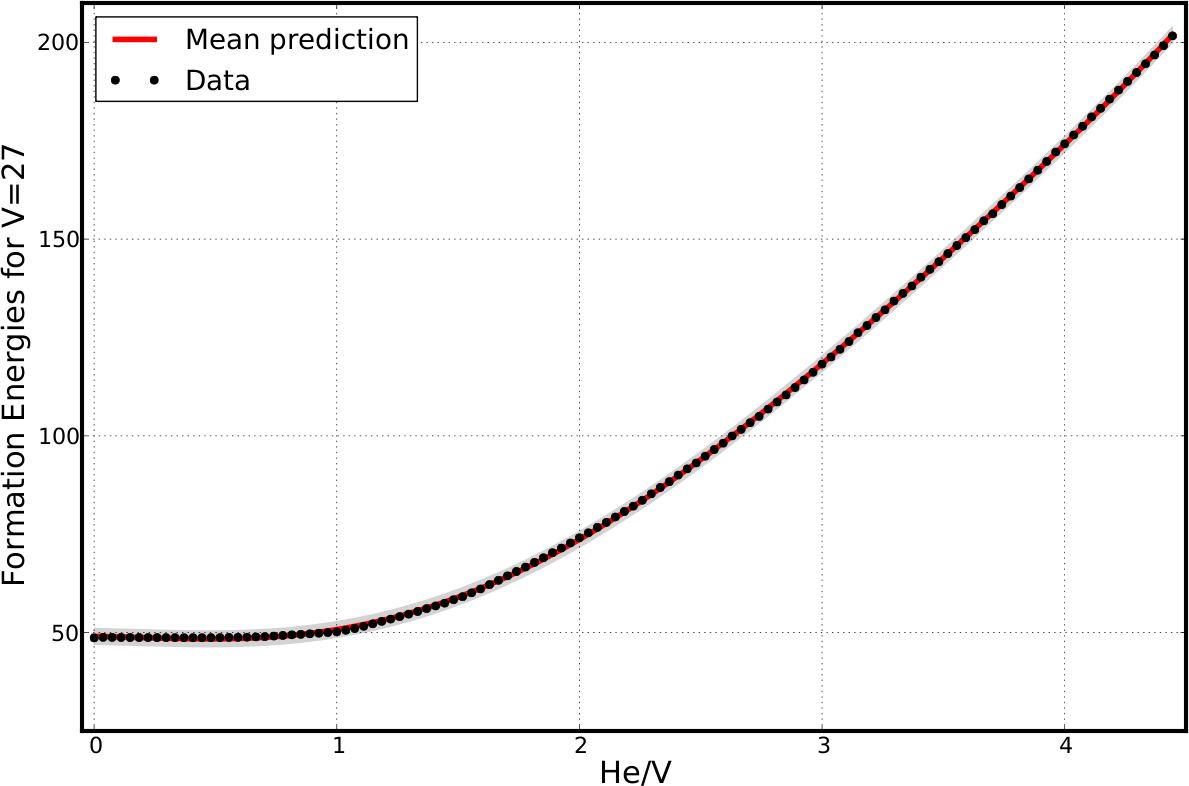
\includegraphics[width=0.95\textwidth]{V27_postpred}
%      \end{figure}
% \end{frame}
% 
% \begin{frame}{Bayesian Inference in UQTk: V = 27}
% 	\begin{columns}[c]		
% 		\column{.56\textwidth}
% 			\begin{figure}
% 	 	 		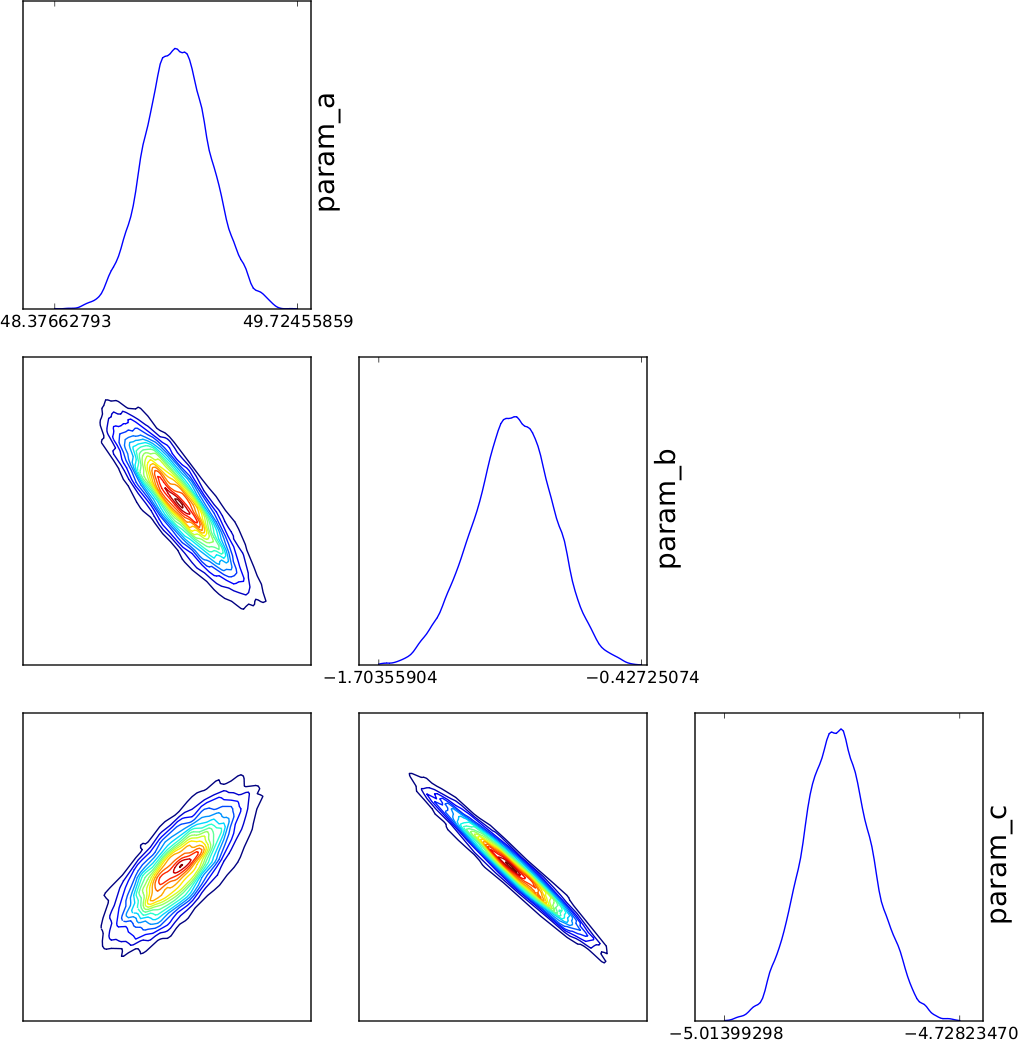
\includegraphics[width=\textwidth]{V27_posteriors}
% 	 		\end{figure}
% 	 	\column{.43\textwidth}
% 	 		\center{$\gamma = 0.1$}
% 	 		\begin{figure}[ht]
% 	 			\subfigure{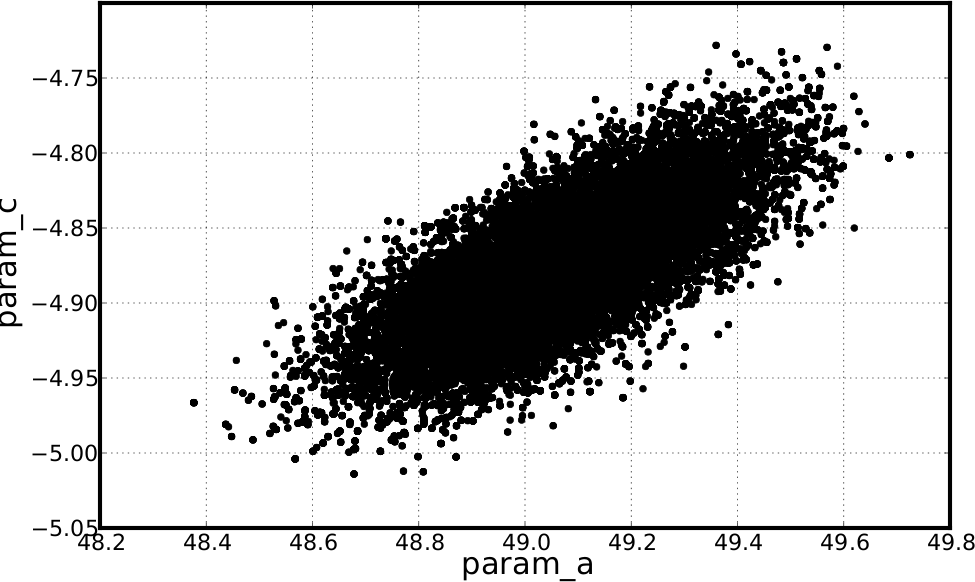
\includegraphics[width=\textwidth]{V27_chn_param_a_param_c}}
% 	 			\newline
% 	 			\newline
%          		\subfigure{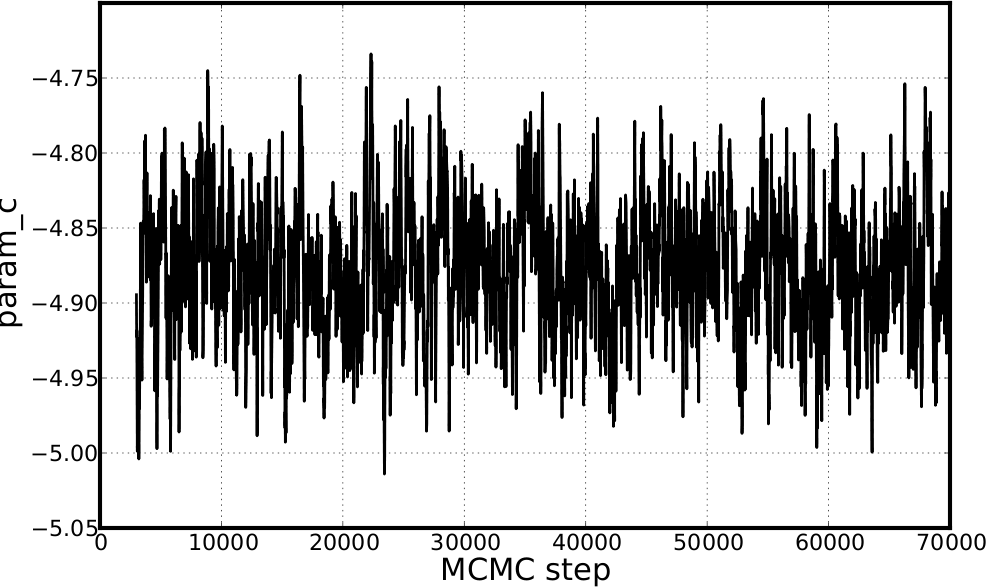
\includegraphics[width=\textwidth]{V27_chn_param_c}}
%      		\end{figure}	 		
% 	\end{columns}
% \end{frame}
% 
% \begin{frame}{Bayesian Inference in UQTk: $V = 27$ Formation Energies}
% 	\large
% 	    \begin{itemize}
%     	\item[$\blacktriangleright$] Suppose the following function is used to fit
%     	the data 
%     	$$f(x) = a + b x + c x^2 + d x^3 + g x^4 + h x^5$$
%     	\item[$\blacktriangleright$] Fitting the data using GNUplot gives
%     	\begin{align*}
%     	a = 49.0722, &b = -1.0619, c = -4.87474, d = 9.92562, \\
%     	&g = -2.47767, h = 0.200702
%     	\end{align*}
%     	\item[$\blacktriangleright$] Model the data with
%     	\begin{align*}
%     	M(x) = \texttt{param\_a} &+ \texttt{param\_b} \cdot x - \texttt{param\_c}
%     	\cdot x^2 + \texttt{param\_d} \cdot x^3 \\
%     	 &- 2.47467 \cdot x^4 + 0.200702 \cdot x^5
%     	\end{align*}
%     	to infer 4 parameters.
%     \end{itemize}
% \end{frame}
% 
% \begin{frame}{Bayesian Inference in UQTk: V = 27}
%      \begin{figure}
%          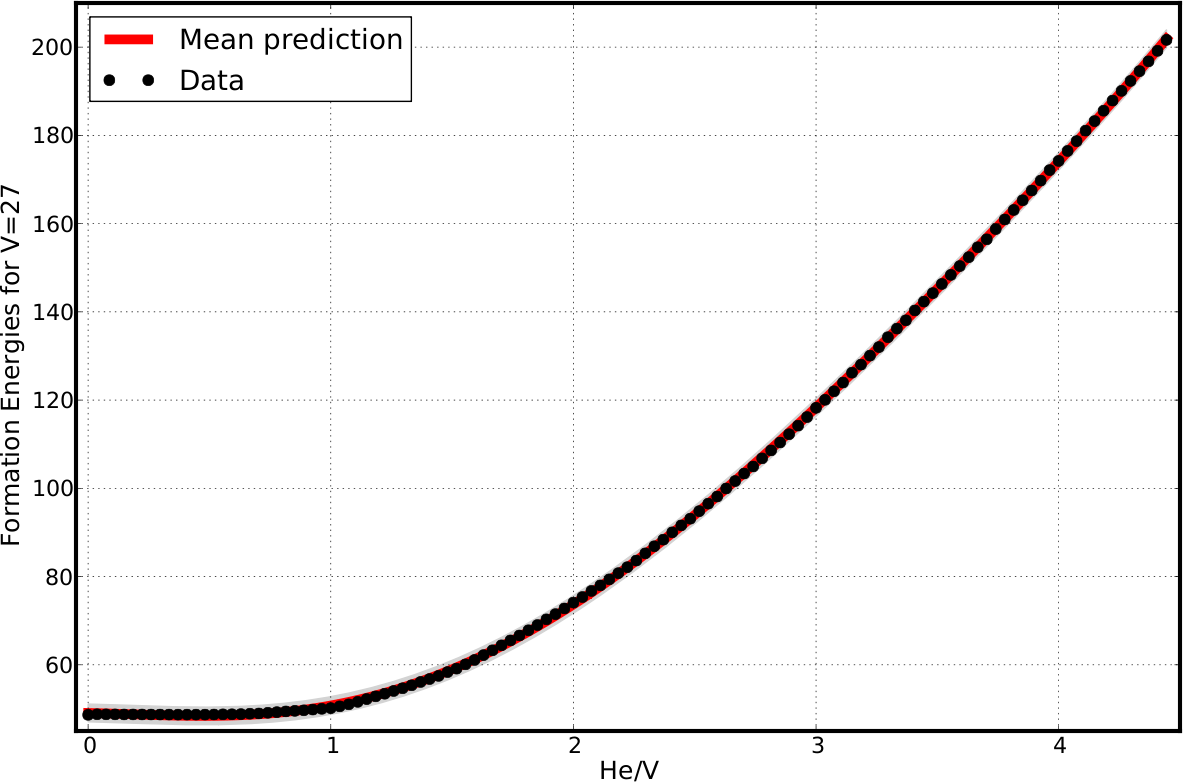
\includegraphics[width=0.95\textwidth]{V27_postpredabcd}
%      \end{figure}
% \end{frame}
% 
% \begin{frame}{Bayesian Inference in UQTk: V = 27}
% 	\begin{columns}[c]
% 		\column{.6\textwidth}
% 			\begin{figure}
% 	 	 		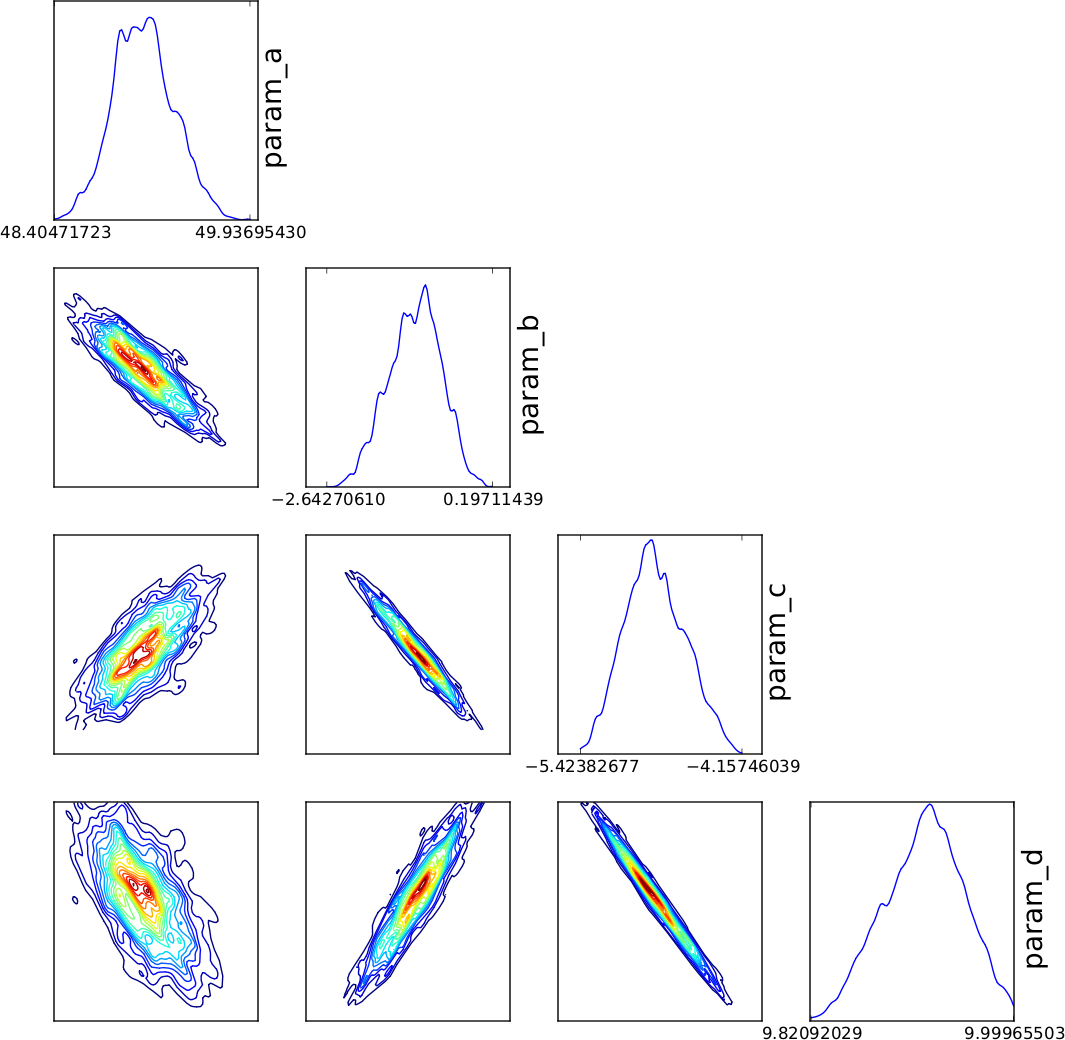
\includegraphics[width=\textwidth]{V27abcd_posteriors}
% 	 		\end{figure} 	
% 	 	\column{.39\textwidth}
% 	 		\center{$\gamma = 0.1$}
% 	 		\begin{figure}[ht]
% 	 			\subfigure{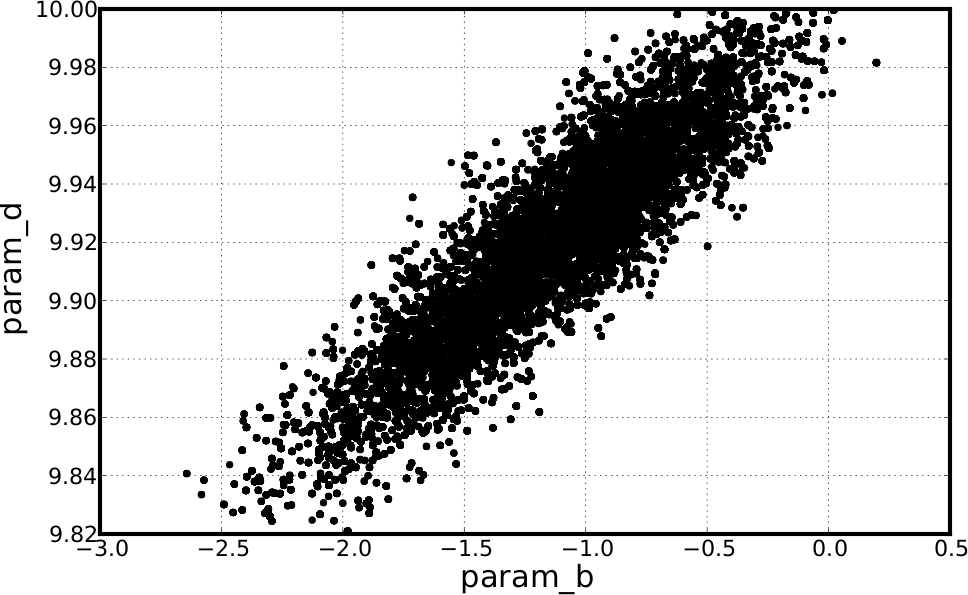
\includegraphics[width=\textwidth]{V27abcd_chnparamb_d}}
% 	 			\newline
% 	 			\newline
%          		\subfigure{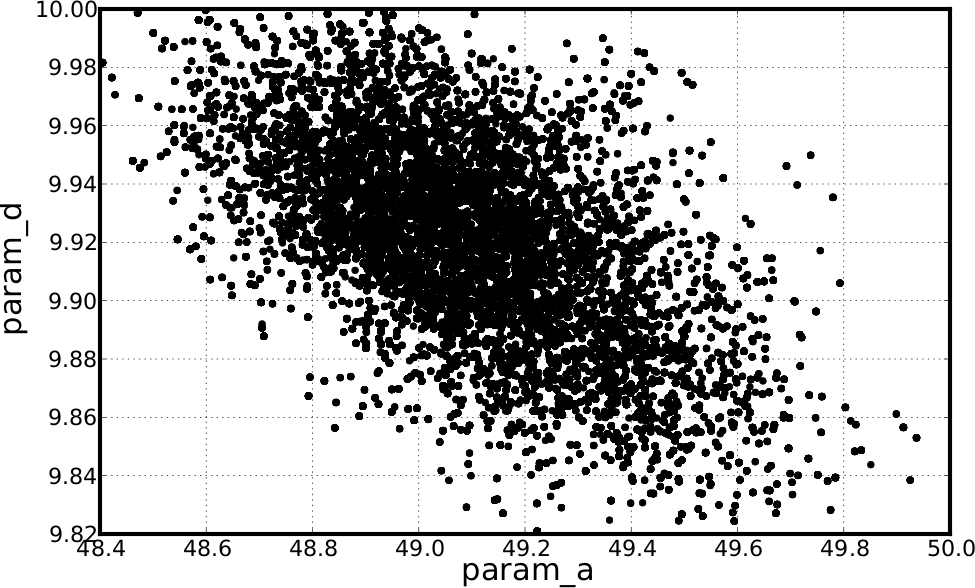
\includegraphics[width=\textwidth]{V27_chnparama_d}}
%      		\end{figure}   		
% 	\end{columns}
% \end{frame}
% 
% \begin{frame}{Bayesian Inference in UQTk: V = 27}
% 	\begin{columns}[c]
% 	 	\column{.5\textwidth}
% 	 		\begin{figure}[ht]
% 	 			\subfigure{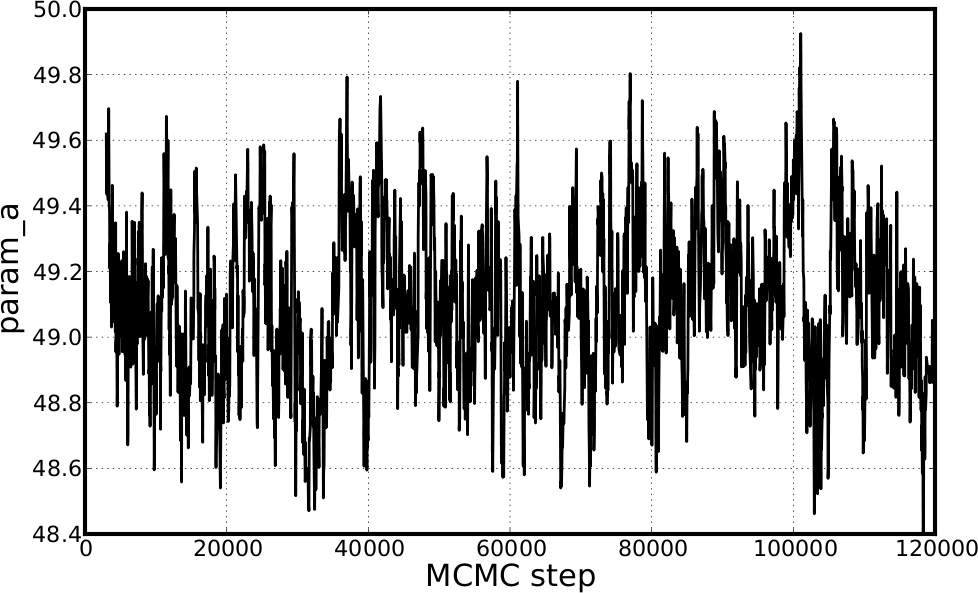
\includegraphics[width=\textwidth]{V27abcd_chnparama}}
% 	 			\newline
%          		\subfigure{\includegraphics[width=\textwidth]{V27abcd_chnparamc}}
%      		\end{figure}
% 		\column{.5\textwidth}
% 	 		\begin{figure}[ht]
% 	 			\subfigure{\includegraphics[width=\textwidth]{V27abcd_chnparam_b}}
% 	 			\newline
%          		\subfigure{\includegraphics[width=\textwidth]{V27abcd_chnparam_d}}
%      		\end{figure}		  		
% 	\end{columns}
% \end{frame}
% 
% \begin{frame}{Bayesian Inference in UQTk: V = 27, Infer 5 params}
%      \begin{figure}
%          \includegraphics[width=0.95\textwidth]{V27most_postpred}
%      \end{figure}
% \end{frame}
% 
% \begin{frame}{Bayesian Inference in UQTk: V = 27, infer 5 params}
% 	\begin{columns}[c]
% 		\column{.6\textwidth}
% 			\begin{figure}
% 	 	 		\includegraphics[width=\textwidth]{V27most_posteriors}
% 	 		\end{figure} 	
% 	 	\column{.39\textwidth}
% 	 		\center{$\gamma = 0.1$}
% 	 		\begin{figure}[ht]
% 	 			\subfigure{\includegraphics[width=\textwidth]{V27most_chnparama_d}}
% 	 			\newline
% 	 			\newline
%          		\subfigure{\includegraphics[width=\textwidth]{V27most_chnparama}}
%      		\end{figure}   		
% 	\end{columns}
% \end{frame}
% 
% \begin{frame}{Bayesian Inference on Formation Energies}
% 	\large
% 	\begin{itemize}
% 	  \item[$\blacktriangleright$] Using Bayesian inference to infer the parameters
% 	  of the formation energy fit has proven to be a nontrivial task \newline
% 	  \item[$\blacktriangleright$] After many unsuccessful attempts to infer
% 	  the fit parameters for just one vacancy number further investigation into
% 	  the formation energy noise was performed
% 	\end{itemize}
% \end{frame}
% 
% \begin{frame}{Formation Energy Noise for V = 1, 2, 6, 14}
%      \begin{figure}
%          \includegraphics[width=0.43\textwidth]{V1noise}
%          \hspace{4mm}
%          \includegraphics[width=0.43\textwidth]{V2noise}
%      \end{figure}
%      \vspace{-2mm}
%      \begin{figure}
%          \includegraphics[width=0.43\textwidth]{V6noise}
%          \hspace{4mm}
%          \includegraphics[width=0.43\textwidth]{V14noise}
%      \end{figure}
% \end{frame}
% 
% \begin{frame}{Formation Energy Noise for V = 18, 19, 27, 32, 44}
%      \vspace{-2mm}
%      \begin{figure}[!htp]
%          \includegraphics[width=0.33\textwidth]{V18noise}
%          \hspace{4mm}
%          \includegraphics[width=0.33\textwidth]{V19noise}
%      \end{figure}
%      \vspace{-3mm}
%      \begin{figure}[!htp]
%          \includegraphics[width=0.33\textwidth]{V27noise}
%          \includegraphics[width=0.33\textwidth]{V32noise}
%          \includegraphics[width=0.33\textwidth]{V44noise}
%      \end{figure}
% \end{frame}
% 
% \begin{frame}{Fit vs. Bayesian Noise for V = 27}
% 	\begin{figure}
% 		\includegraphics[width=0.5\linewidth]{V27fitnoise}
% 	\end{figure}
% 	\vspace{-4mm}
% 	\begin{figure}
% 		\includegraphics[width=0.5\linewidth]{V27_bayesian_noise}
% 	\end{figure}
% \end{frame}
% 
% 
% \begin{frame}{Bayesian Inference in UQTk: V = 18, infer 6 params}
% 	\begin{columns}[c]
% 		\column{.6\textwidth}
% 			\begin{figure}
% 	 	 		\includegraphics[width=\textwidth]{v18chain}
% 	 		\end{figure} 	
% 	 	\column{.39\textwidth}
% 	 		\begin{figure}[ht]
% 	 			\subfigure{\includegraphics[width=\textwidth]{v18_result6params}}
% 	 			\newline
% 	 			\newline
%          		\subfigure{\includegraphics[width=\textwidth]{v18_noise6params}}
%      		\end{figure}   		
% 	\end{columns}
% \end{frame}
% 
% \begin{frame}{Bayesian Inference in UQTk: V = 32, infer 6 params}
% 	\begin{columns}[c]
% 		\column{.6\textwidth}
% 			\begin{figure}
% 	 	 		\includegraphics[width=\textwidth]{v32chain}
% 	 		\end{figure} 	
% 	 	\column{.39\textwidth}
% 	 		\begin{figure}[ht]
% 	 			\subfigure{\includegraphics[width=\textwidth]{v32_6params}}
% 	 			\newline
% 	 			\newline
%          		\subfigure{\includegraphics[width=\textwidth]{v32noise6params}}
%      		\end{figure}   		
% 	\end{columns}
% \end{frame}
% 
% \begin{frame}{Piecewise Bayesian Inference V~$= 1$}
%   	\begin{columns}[onlytextwith]
%     	\begin{column}{0.43\textwidth}
%     	$$He/V \leq 1$$
%     	\vspace{1.2cm}
%       		\begin{figure}
%         		\includegraphics[width=0.9\textwidth]{low1Triangle}
%       		\end{figure}
%     	\end{column}  
%     	\begin{column}{0.59\textwidth}
%     	$$He/V \geq 1$$
%       		\begin{figure}
%         		\includegraphics[width=0.9\textwidth]{high1Triangle}
%       		\end{figure}
%     	\end{column}
%   	\end{columns}
% \end{frame}
% 
% \begin{frame}{Piecewise Bayesian Inference V~$= 1$}
%   	\begin{columns}[onlytextwith]
%     	\begin{column}{0.5\textwidth}
%     	$$He/V \leq 1$$
%       		\begin{figure}
%         		\includegraphics[width=0.9\textwidth]{low1Result}
%       		\end{figure}
%       		~~~~~~~~~~~~~~~~~~~$2$~points
%     	\end{column}  
%     	\begin{column}{0.5\textwidth}
%     	$$He/V \geq 1$$
%       		\begin{figure}
%         		\includegraphics[width=0.9\textwidth]{high1Result}
%       		\end{figure}
%       		~~~~~~~~~~~~~~~~~~~$9$~points
%     	\end{column}
%   	\end{columns}
% \end{frame}
% 
% \begin{frame}{Piecewise Bayesian Inference V~$= 1$}
%   	\begin{columns}[onlytextwith]
%     	\begin{column}{0.5\textwidth}
%     	$$He/V \leq 1$$
%       		\begin{figure}
%         		\includegraphics[width=0.9\textwidth]{low1ResultDiff}
%       		\end{figure}
%       		~~~~~~~~~~~~~~~~~~~$2$~points
%     	\end{column}  
%     	\begin{column}{0.5\textwidth}
%     	$$He/V \geq 1$$
%       		\begin{figure}
%         		\includegraphics[width=0.9\textwidth]{high1ResultDiff}
%       		\end{figure}
%       		~~~~~~~~~~~~~~~~~~~$9$~points
%     	\end{column}
%   	\end{columns}
% \end{frame}
% 
% \begin{frame}{Piecewise Bayesian Inference V~$= 44$}
%   	\begin{columns}[onlytextwith]
%     	\begin{column}{0.43\textwidth}
%     	$$He/V \leq 1$$
%     	\vspace{1.2cm}
%       		\begin{figure}
%         		\includegraphics[width=0.9\textwidth]{low44Triangle}
%       		\end{figure}
%     	\end{column}  
%     	\begin{column}{0.59\textwidth}
%     	$$He/V \geq 1$$
%       		\begin{figure}
%         		\includegraphics[width=0.9\textwidth]{high44Triangle}
%       		\end{figure}
%     	\end{column}
%   	\end{columns}
% \end{frame}
% 
% \begin{frame}{Piecewise Bayesian Inference V~$= 44$}
%   	\begin{columns}[onlytextwith]
%     	\begin{column}{0.5\textwidth}
%     	$$He/V \leq 1$$
%       		\begin{figure}
%         		\includegraphics[width=0.9\textwidth]{low44Result}
%       		\end{figure}
%       		~~~~~~~~~~~~~~~~~~~$45$~points
%     	\end{column}  
%     	\begin{column}{0.5\textwidth}
%     	$$He/V \geq 1$$
%       		\begin{figure}
%         		\includegraphics[width=0.9\textwidth]{high44Result}
%       		\end{figure}
%       		~~~~~~~~~~~~~~~~~~~$146$~points
%     	\end{column}
%   	\end{columns}
% \end{frame}
% 
% \begin{frame}{Piecewise Bayesian Inference V~$= 44$}
%   	\begin{columns}[onlytextwith]
%     	\begin{column}{0.5\textwidth}
%     	$$He/V \leq 1$$
%       		\begin{figure}
%         		\includegraphics[width=0.9\textwidth]{low44ResultDiff}
%       		\end{figure}
%       		~~~~~~~~~~~~~~~~~~~$45$~points
%     	\end{column}  
%     	\begin{column}{0.5\textwidth}
%     	$$He/V \geq 1$$
%       		\begin{figure}
%         		\includegraphics[width=0.9\textwidth]{high44ResultDiff}
%       		\end{figure}
%       		~~~~~~~~~~~~~~~~~~~$146$~points
%     	\end{column}
%   	\end{columns}
% \end{frame}

\begin{frame}{}
\begin{center}
  \huge{\textbf{Back-Up}}
\end{center}
\end{frame}

\begin{frame}{Excluding V~$=1, 2$, up to V~$=87$}
	\begin{figure}
        \includegraphics[width=0.95\textwidth]{parameters80}
    \end{figure}
\end{frame}

\begin{frame}{Excluding V~$=1, 2$, up to V~$=87$}
	\begin{figure}
        \includegraphics[width=0.95\textwidth]{energy80}
    \end{figure}
\end{frame}

\begin{frame}{Excluding V~$=1, 2$, up to V~$=87$}
	\begin{figure}
        \includegraphics[width=0.95\textwidth]{ratio80}
    \end{figure}
\end{frame}

\end{document}